\chapter{The Search for Invisible Decays of the Higgs Boson}
\label{sec:vbf}

In this chapter, we use events with two forward jets and large missing momentum to probe the coupling of the Higgs boson to invisible particles with sufficiently low masses. 
The discovery of the SM Higgs boson~\cite{higgsdisc} involved multiple production modes.
Gluon fusion has the largest cross section (49 pb) at the LHC because of the large gluon PDF, followed by vector boson fusion (VBF) (3.8 pb), $WH$ (1.4 pb), and $ZH$ (0.89 pb)~\cite{lhchxswg}.
While gluon fusion is the most frequent mode, the unique detector signatures of the other production modes can be combined with various Higgs decay signatures to define signal topologies with smaller backgrounds.

Many DM models~\cite{higgsdm1,higgsdm2,higgsdm3} allow for DM fermions or scalars to acquire mass through the Higgs mechanism, coupling to the SM Higgs boson.
If the DM candidate $\chi$ satisfies $2m_\chi < m_H$, then we expect to observe $H\rightarrow\chi\bar\chi$.
From measurements of the visible branching fractions, we can indirectly place an upper bound of $\mathcal{B}(H\rightarrow\chi\bar\chi)<0.34$~\cite{higgscomb}.
In this chapter, we describe a direct search for $H\rightarrow\chi\bar\chi$ decays.

As with the case of the mono-top search, the $H\rightarrow\chi\bar\chi$ process manifests as \ptmiss. 
Each of the aforementioned Higgs production modes translates into a $\ptmiss+X$ signature, where $X$ refers to one or more SM particles.
Figure~\ref{fig:vbf:hdiags} shows each of the signatures; in this chapter, we will focus on the VBF production mode.
This unique final state topology provides the best sensitivity to $H\rightarrow\chi\bar\chi$.

\begin{figure}
    \begin{center}
        \begin{subfigure}[t]{0.32\textwidth}
            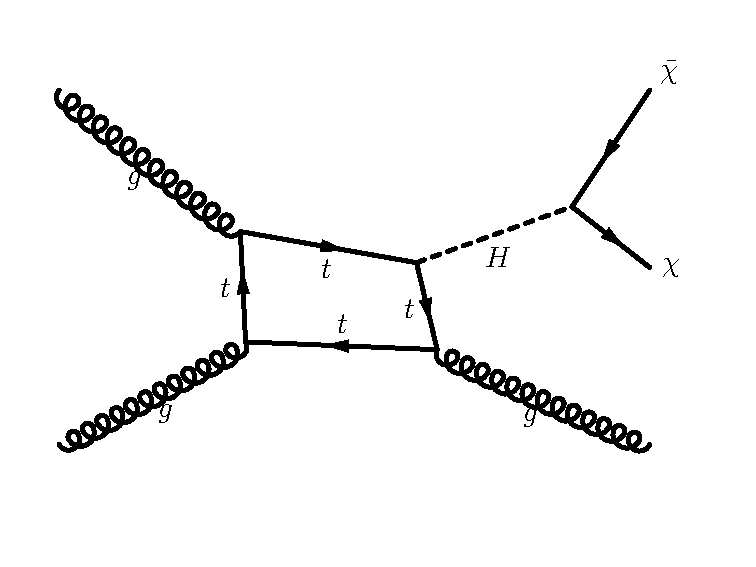
\includegraphics[width=\textwidth]{figures/vbf/diagrams/ggf_hinv.pdf}
            \caption{$gg\rightarrow H(\rightarrow\chi\bar\chi)$+jet(s)}
        \end{subfigure}
        \begin{subfigure}[t]{0.32\textwidth}
            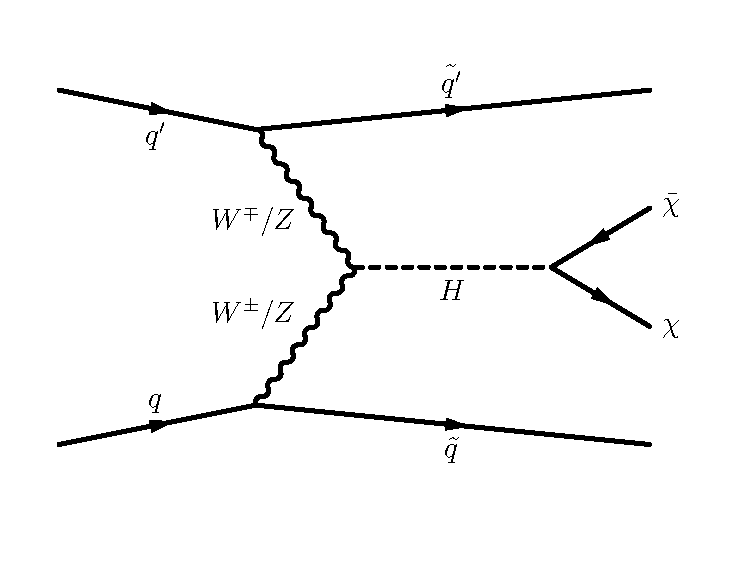
\includegraphics[width=\textwidth]{figures/vbf/diagrams/vbf_hinv.pdf}
            \caption{$qq'\rightarrow H(\rightarrow\chi\bar\chi)$+jet(s)}
        \end{subfigure}
        \begin{subfigure}[t]{0.32\textwidth}
            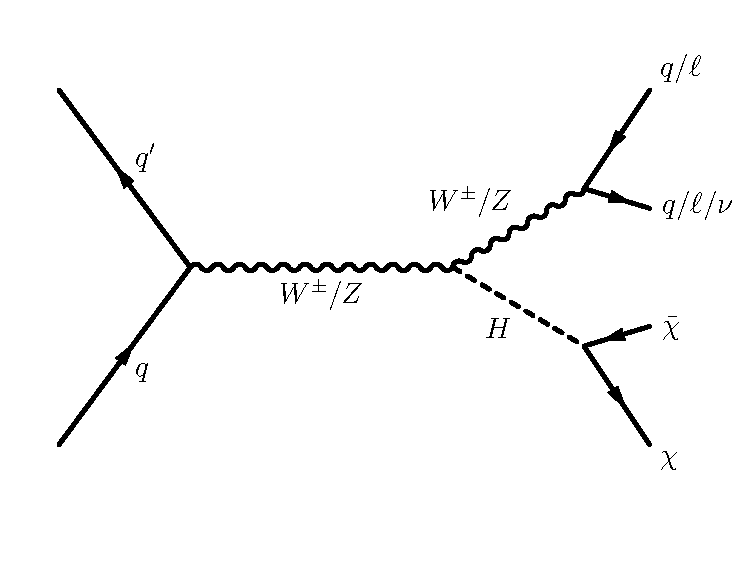
\includegraphics[width=\textwidth]{figures/vbf/diagrams/zh_hinv.pdf}
            \caption{$qq'\rightarrow VH(\rightarrow\chi\bar\chi)$}
        \end{subfigure}
        \caption{Diagrams that contribute to the production of the SM Higgs boson at the LHC, with the subsequent decay to DM candidates.
                 The shown diagrams are all chosen to generate large $\ptmiss$ through the presence of one or more SM particles in the final state.}
        \label{fig:vbf:hdiags}
    \end{center}
\end{figure}

\section{Signal selection}

VBF $\hinv$ events are characterized by large $\ptmiss$ and two jets.
These jets are typically:
\begin{itemize}
    \item Fairly forward in the detector
    \item Far apart from each other in $\eta$
    \item Have large $E$ and moderate $\pt$
    \item Close together in $\phi$
\end{itemize}
A candidate VBF $\hinv$ event displaying these properties is shown in a CMS event display in Figure~\ref{fig:vbf:ed}.
The distributions of kinematics corresponding to these characteristics are shown in Figure~\ref{fig:vbf:sigkins}, compared between the VBF and gluon fusion production modes.

\begin{figure}[]
    \begin{center}
        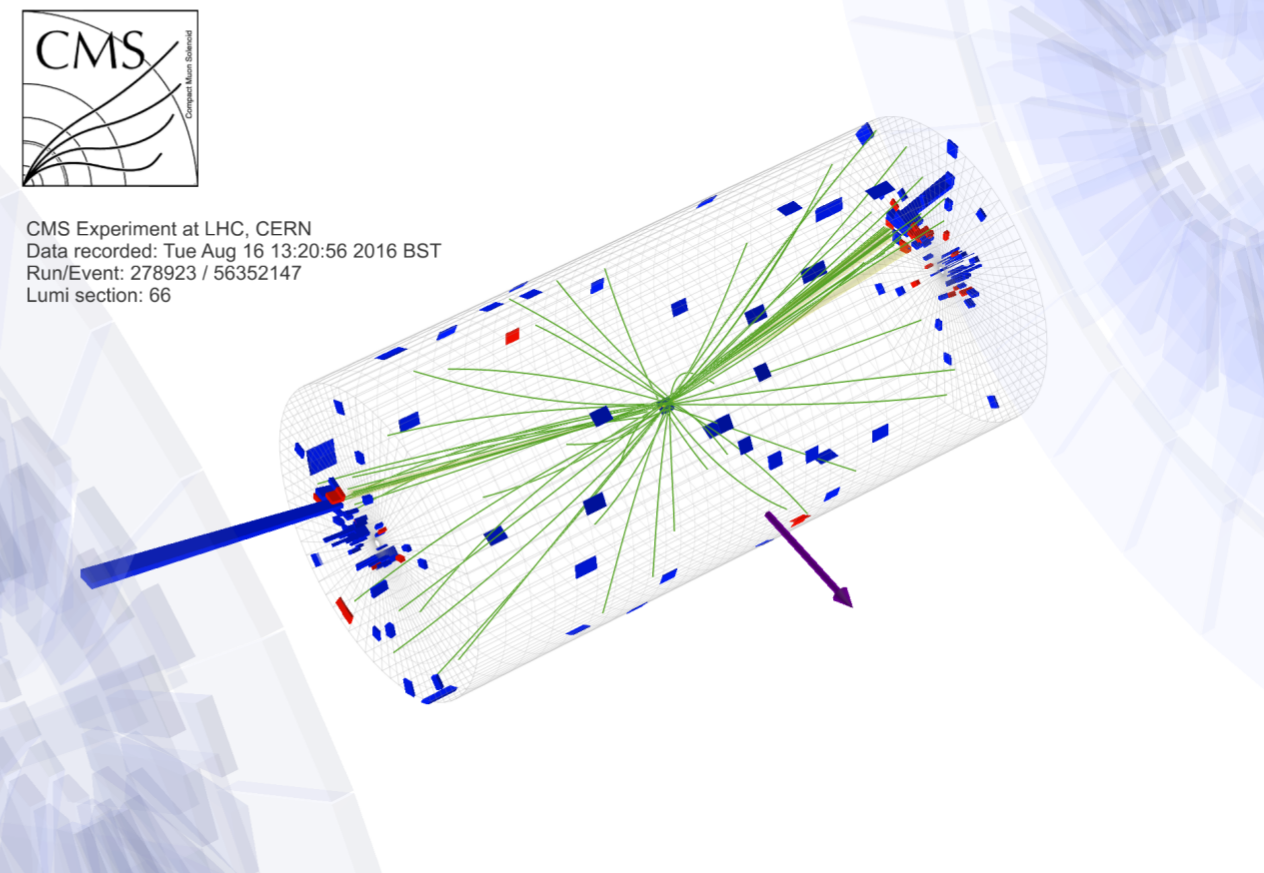
\includegraphics[width=0.8\textwidth]{figures/vbf/misc/event_display.png}
        \caption{Candidate VBF $\hinv$ event with two energetic forward jets ($\pt=180,~107$ GeV) and large $\ptmiss$ ($360$ GeV).
                 Red (blue) towers represent deposits in the hadronic (electromagnetic) calorimeter.
                 Green lines are tracks reconstructed from hits of charged particles in the tracker. 
                 The blue arrow represents the direction and magnitude of the $\ptmiss$.}
        \label{fig:vbf:ed}
    \end{center}
\end{figure}

\begin{figure}[]
    \begin{center}
        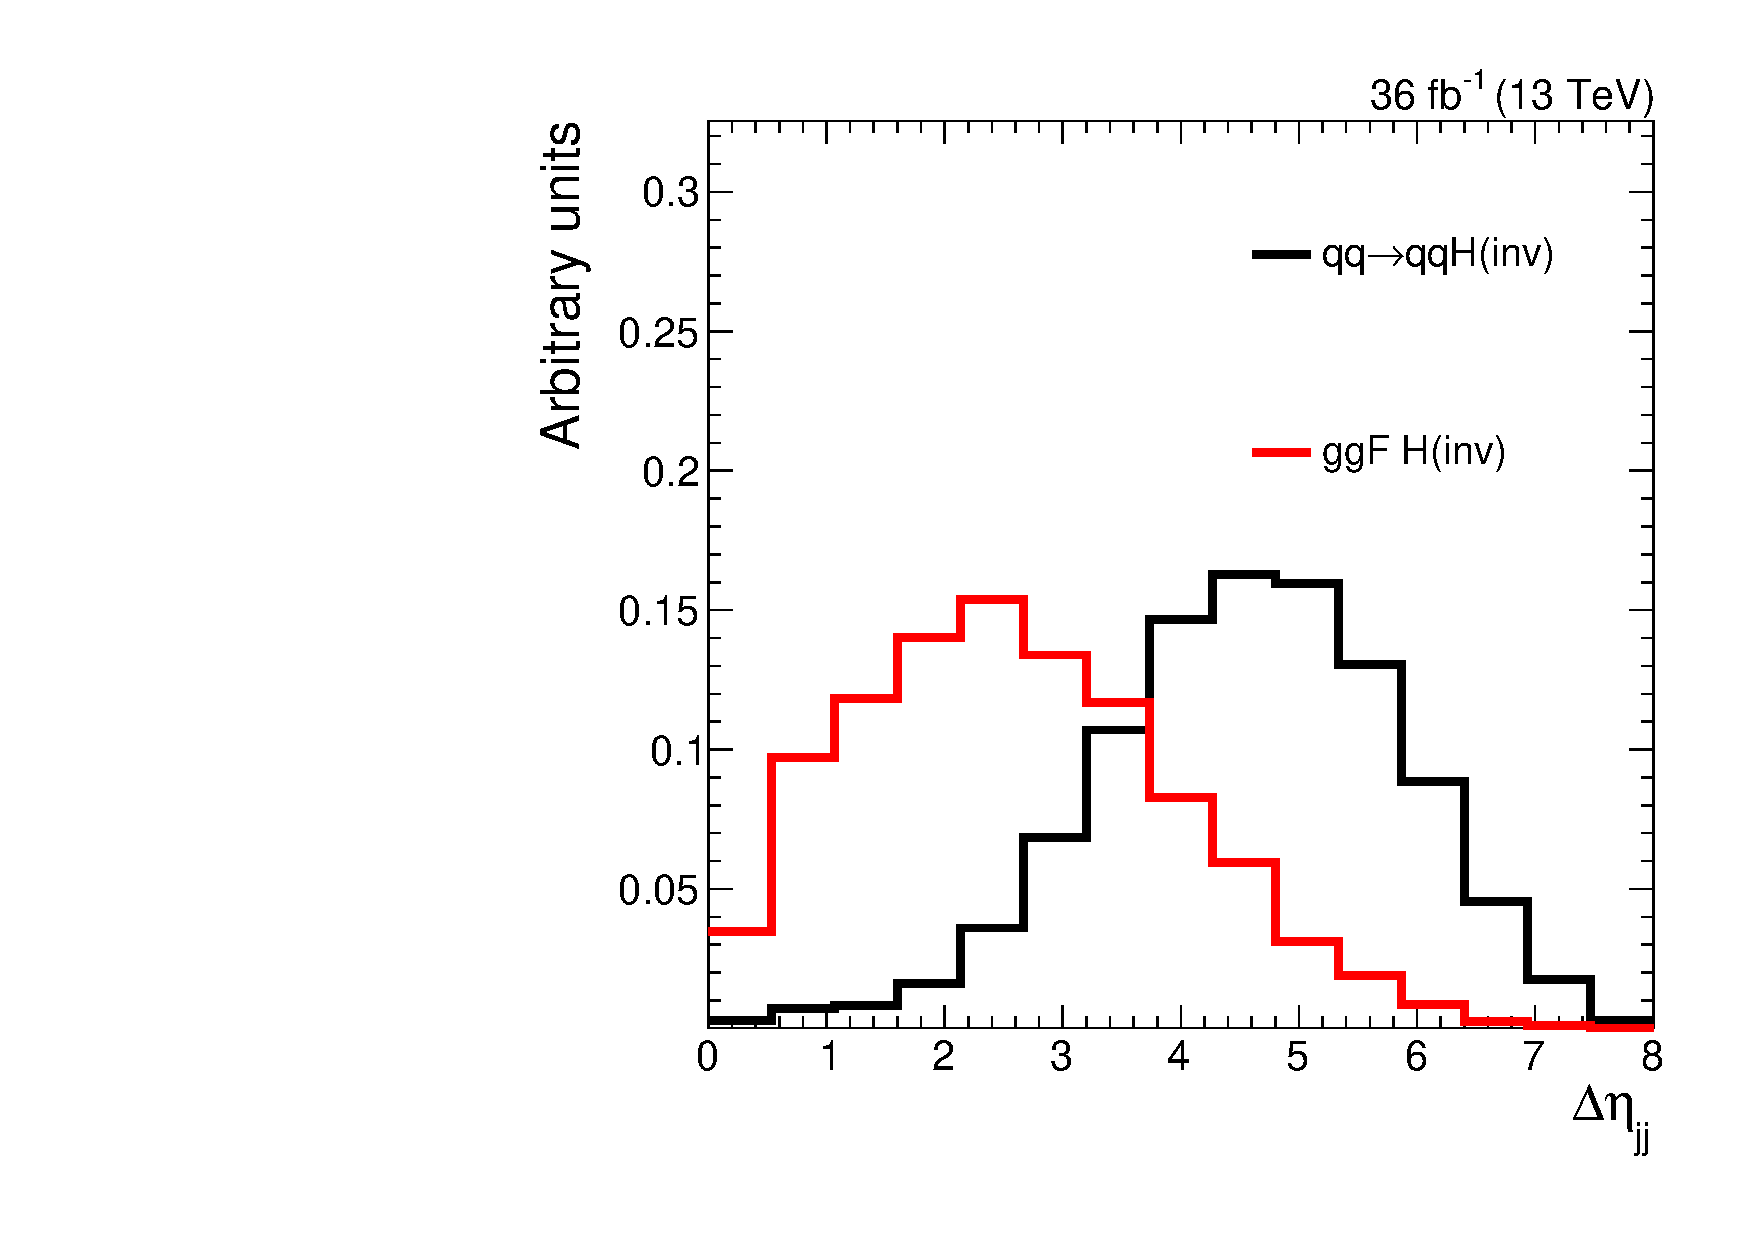
\includegraphics[width=0.32\textwidth]{figures/vbf/shapes_signal/loosesignal_jot12DEta.pdf}
        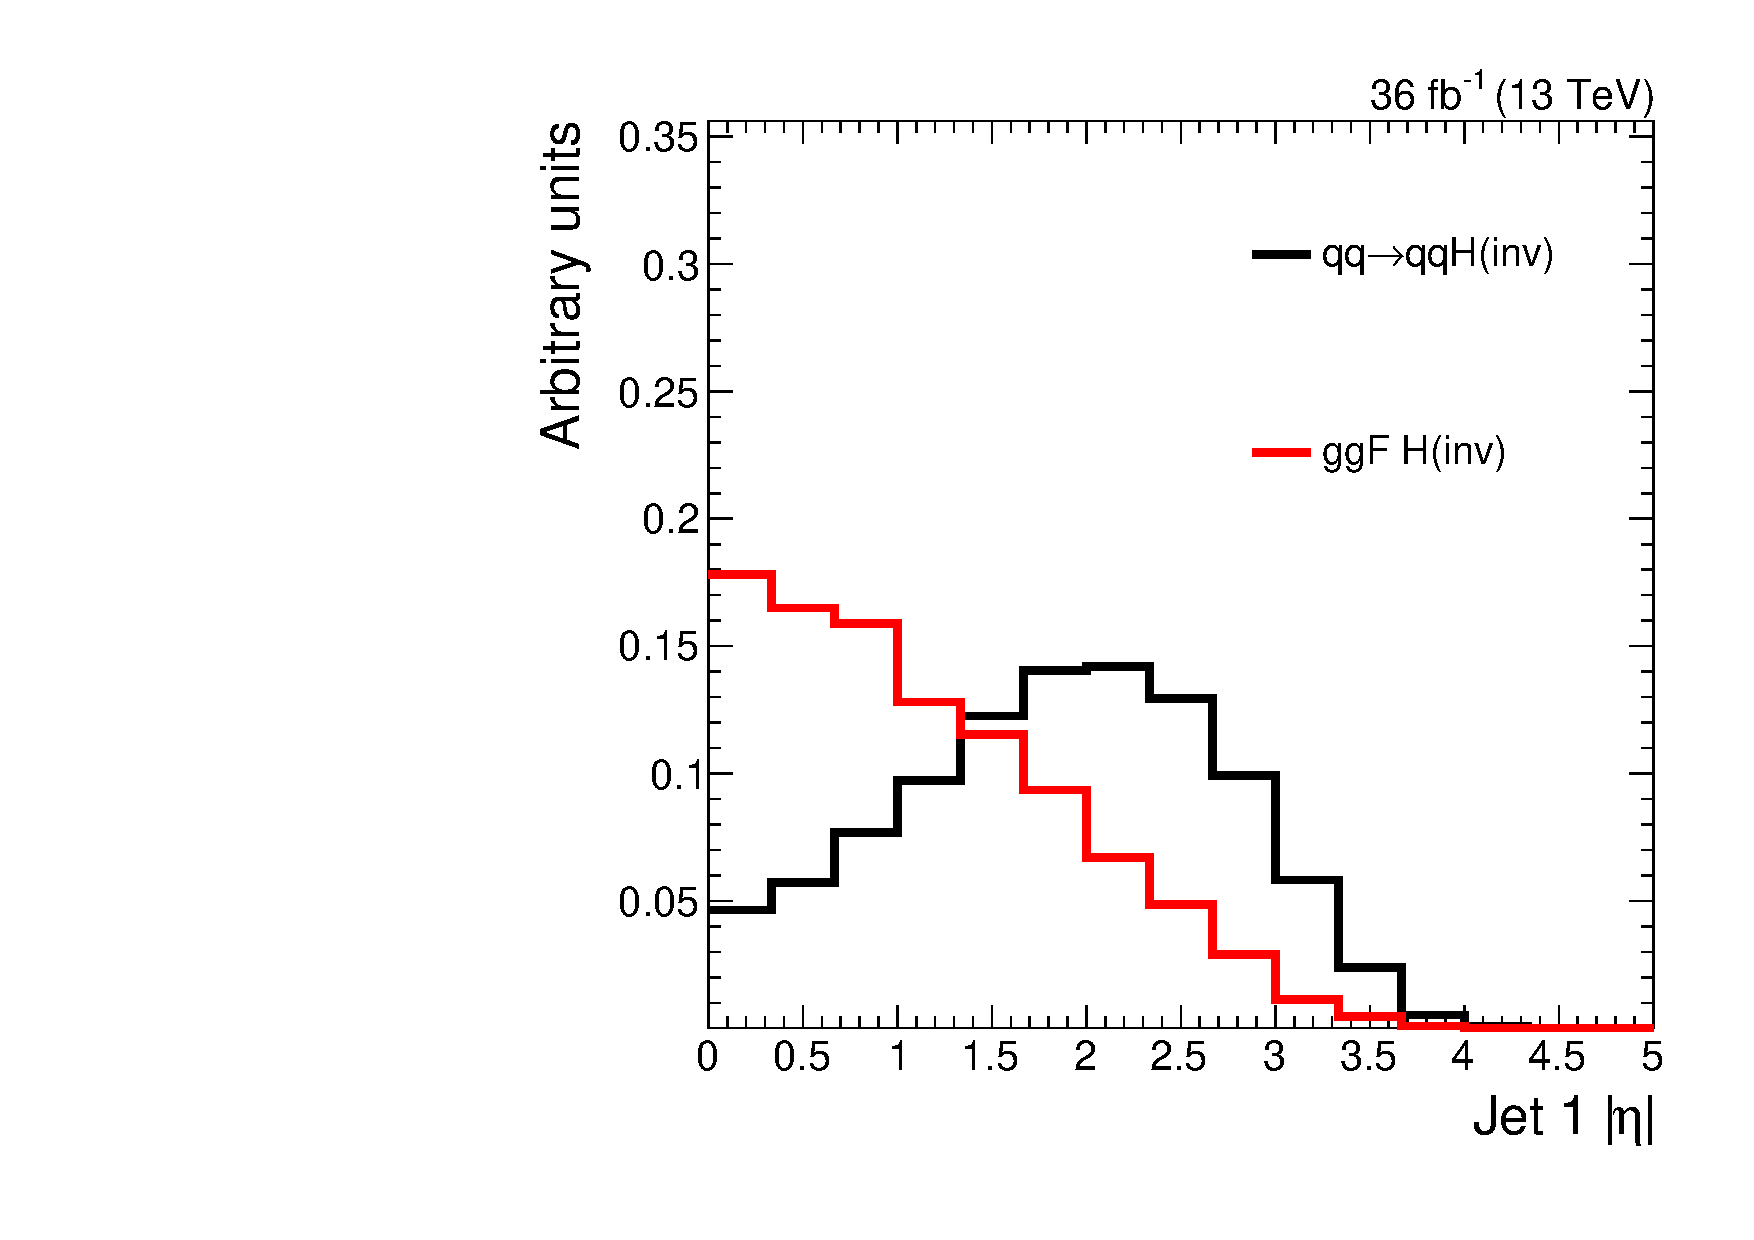
\includegraphics[width=0.32\textwidth]{figures/vbf/shapes_signal/loosesignal_fabsjotEta_0_.pdf}
        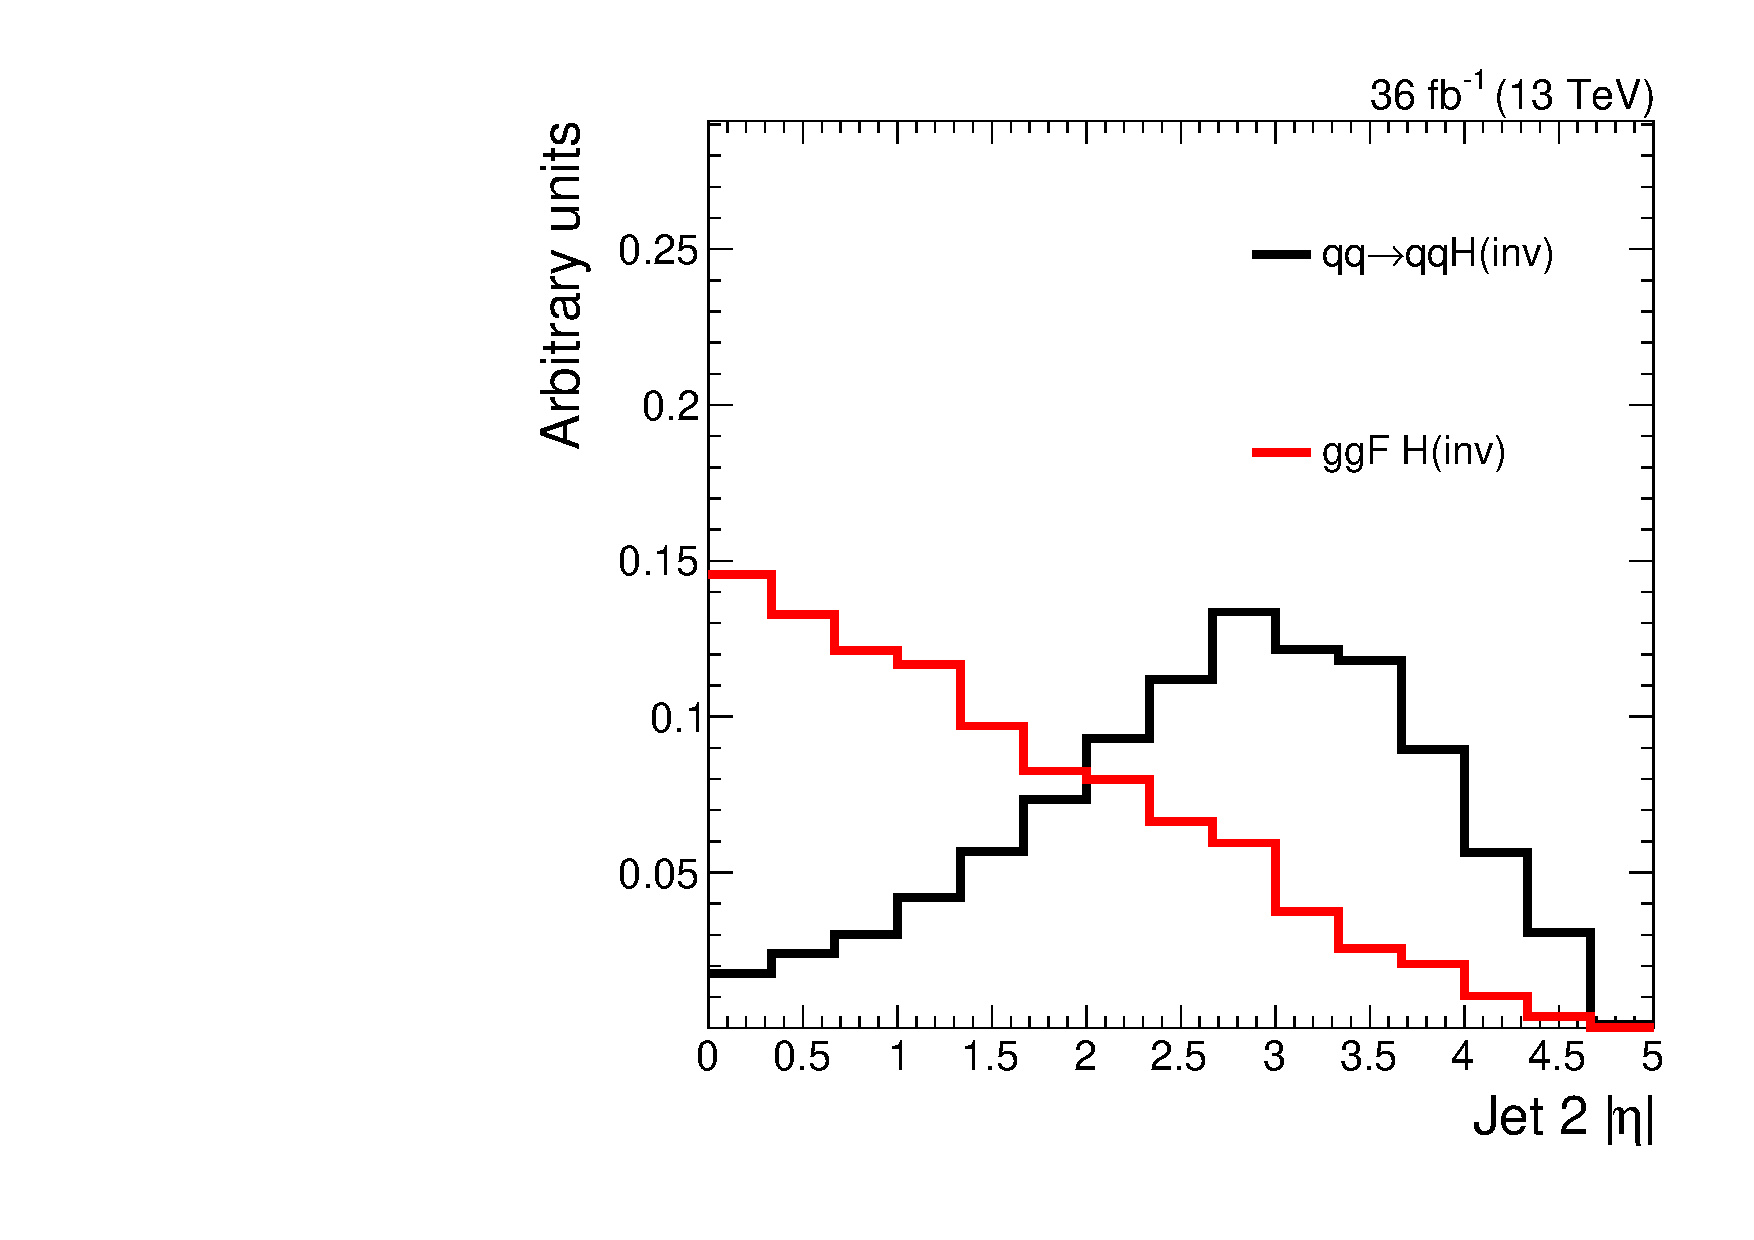
\includegraphics[width=0.32\textwidth]{figures/vbf/shapes_signal/loosesignal_fabsjotEta_1_.pdf} \\
        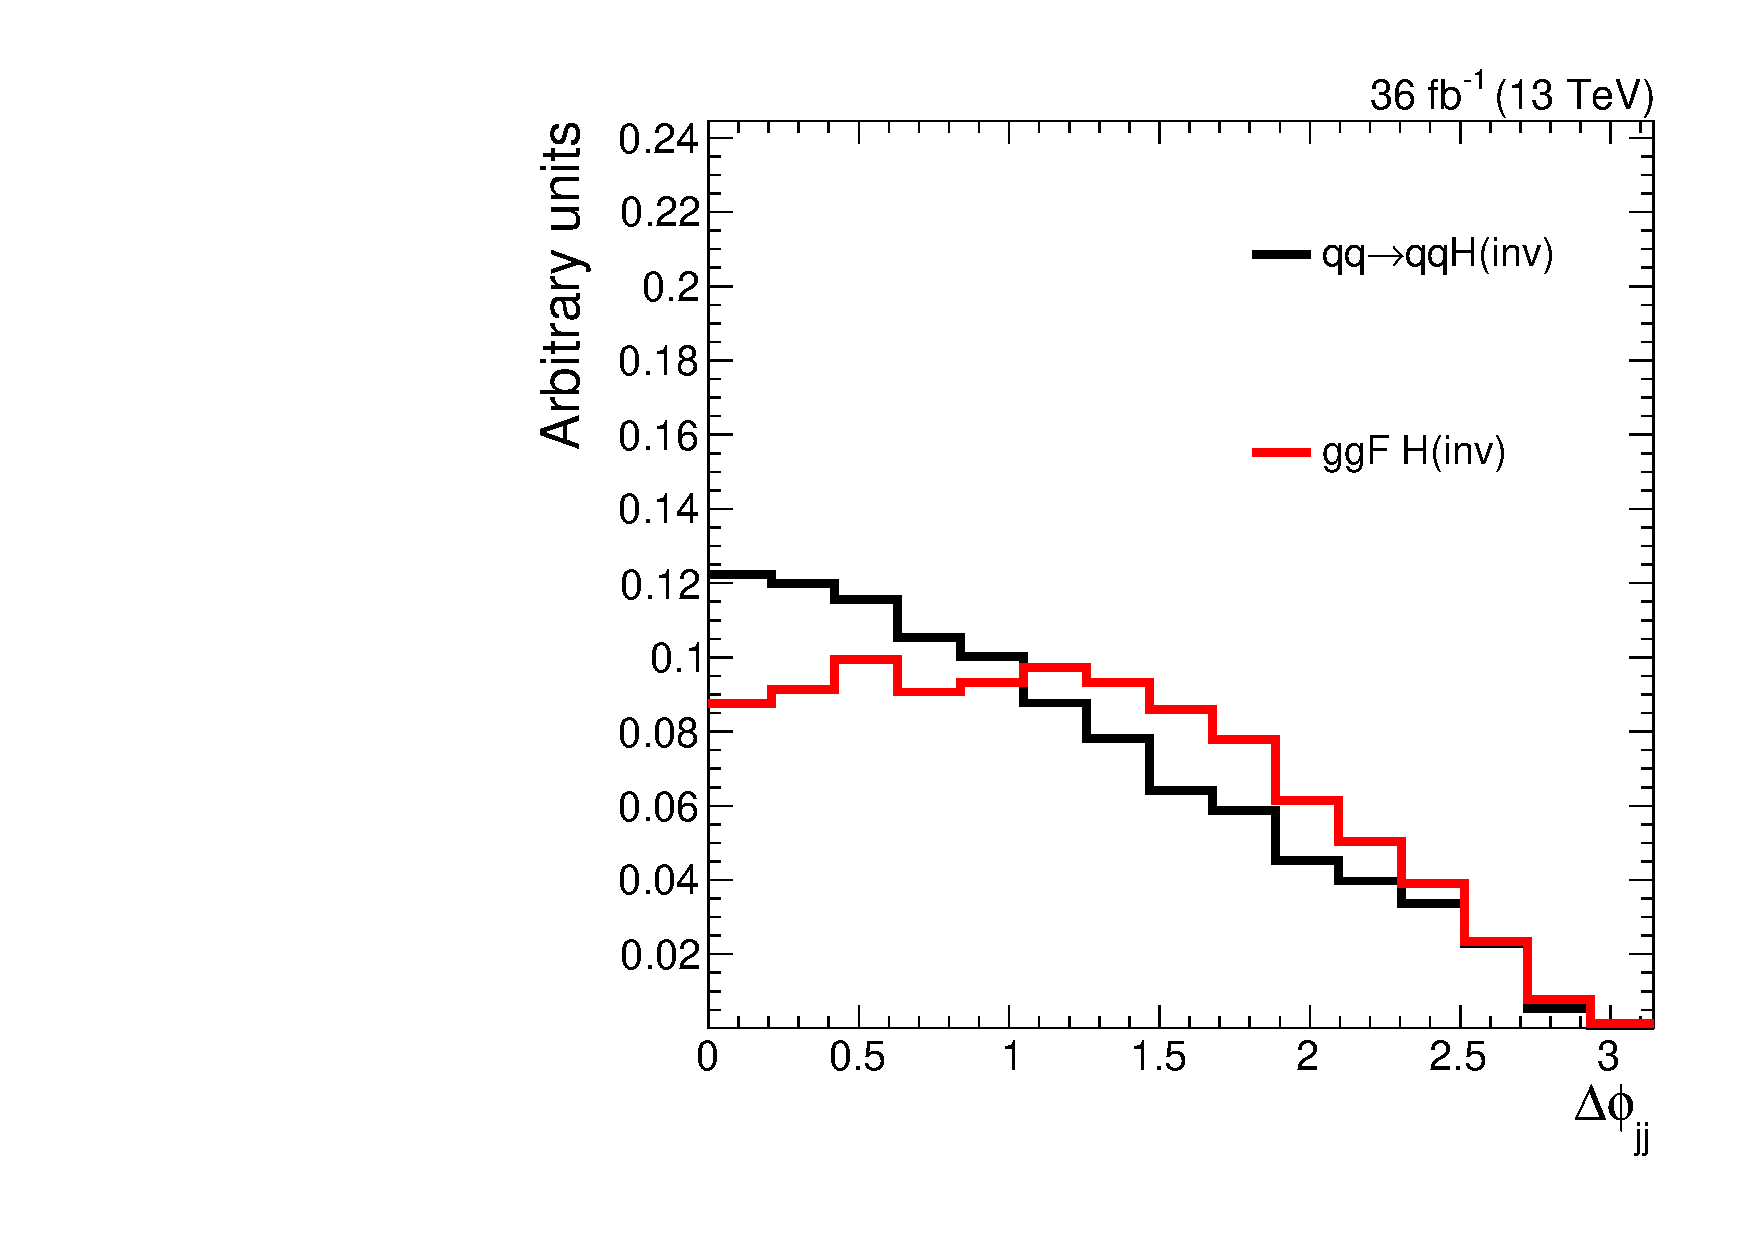
\includegraphics[width=0.32\textwidth]{figures/vbf/shapes_signal/loosesignal_jot12DPhi.pdf}
        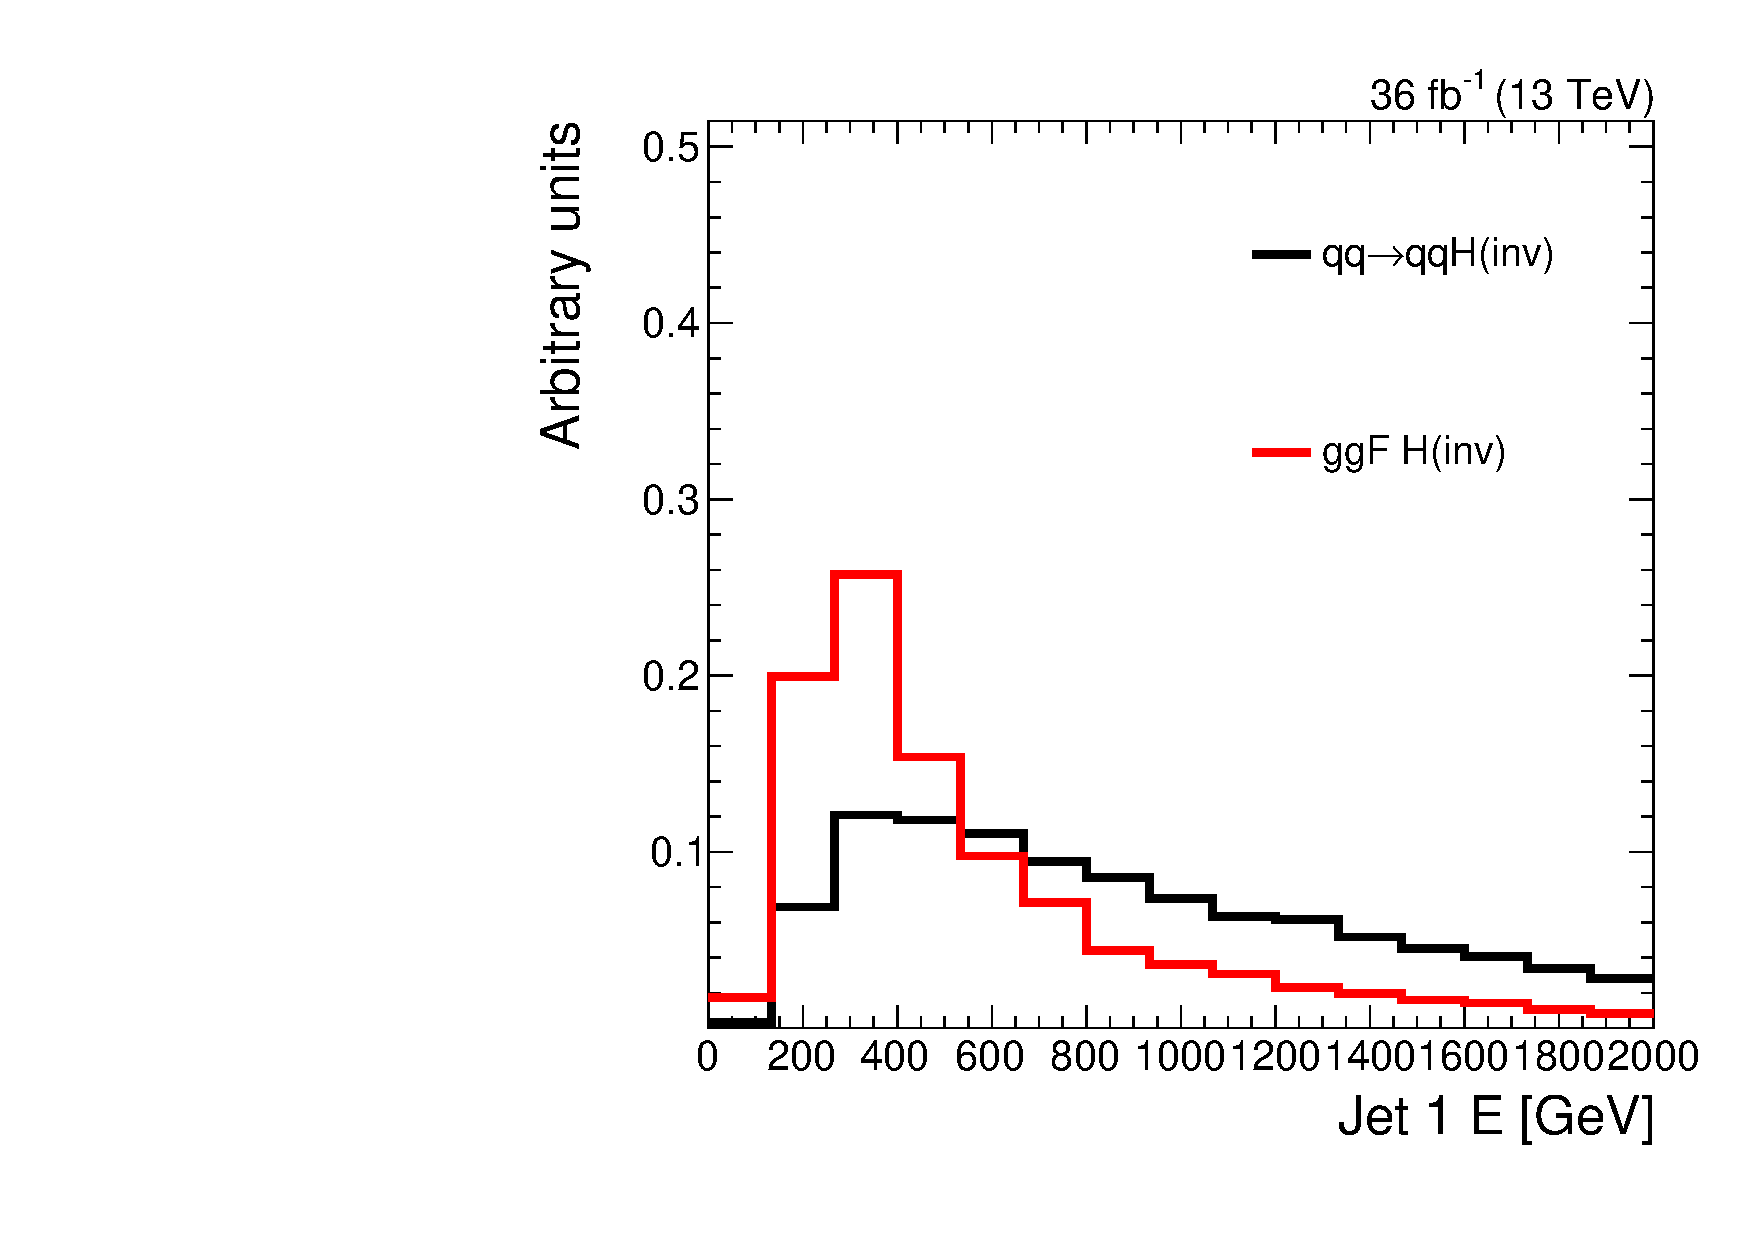
\includegraphics[width=0.32\textwidth]{figures/vbf/shapes_signal/loosesignal_jotE_0_.pdf}
        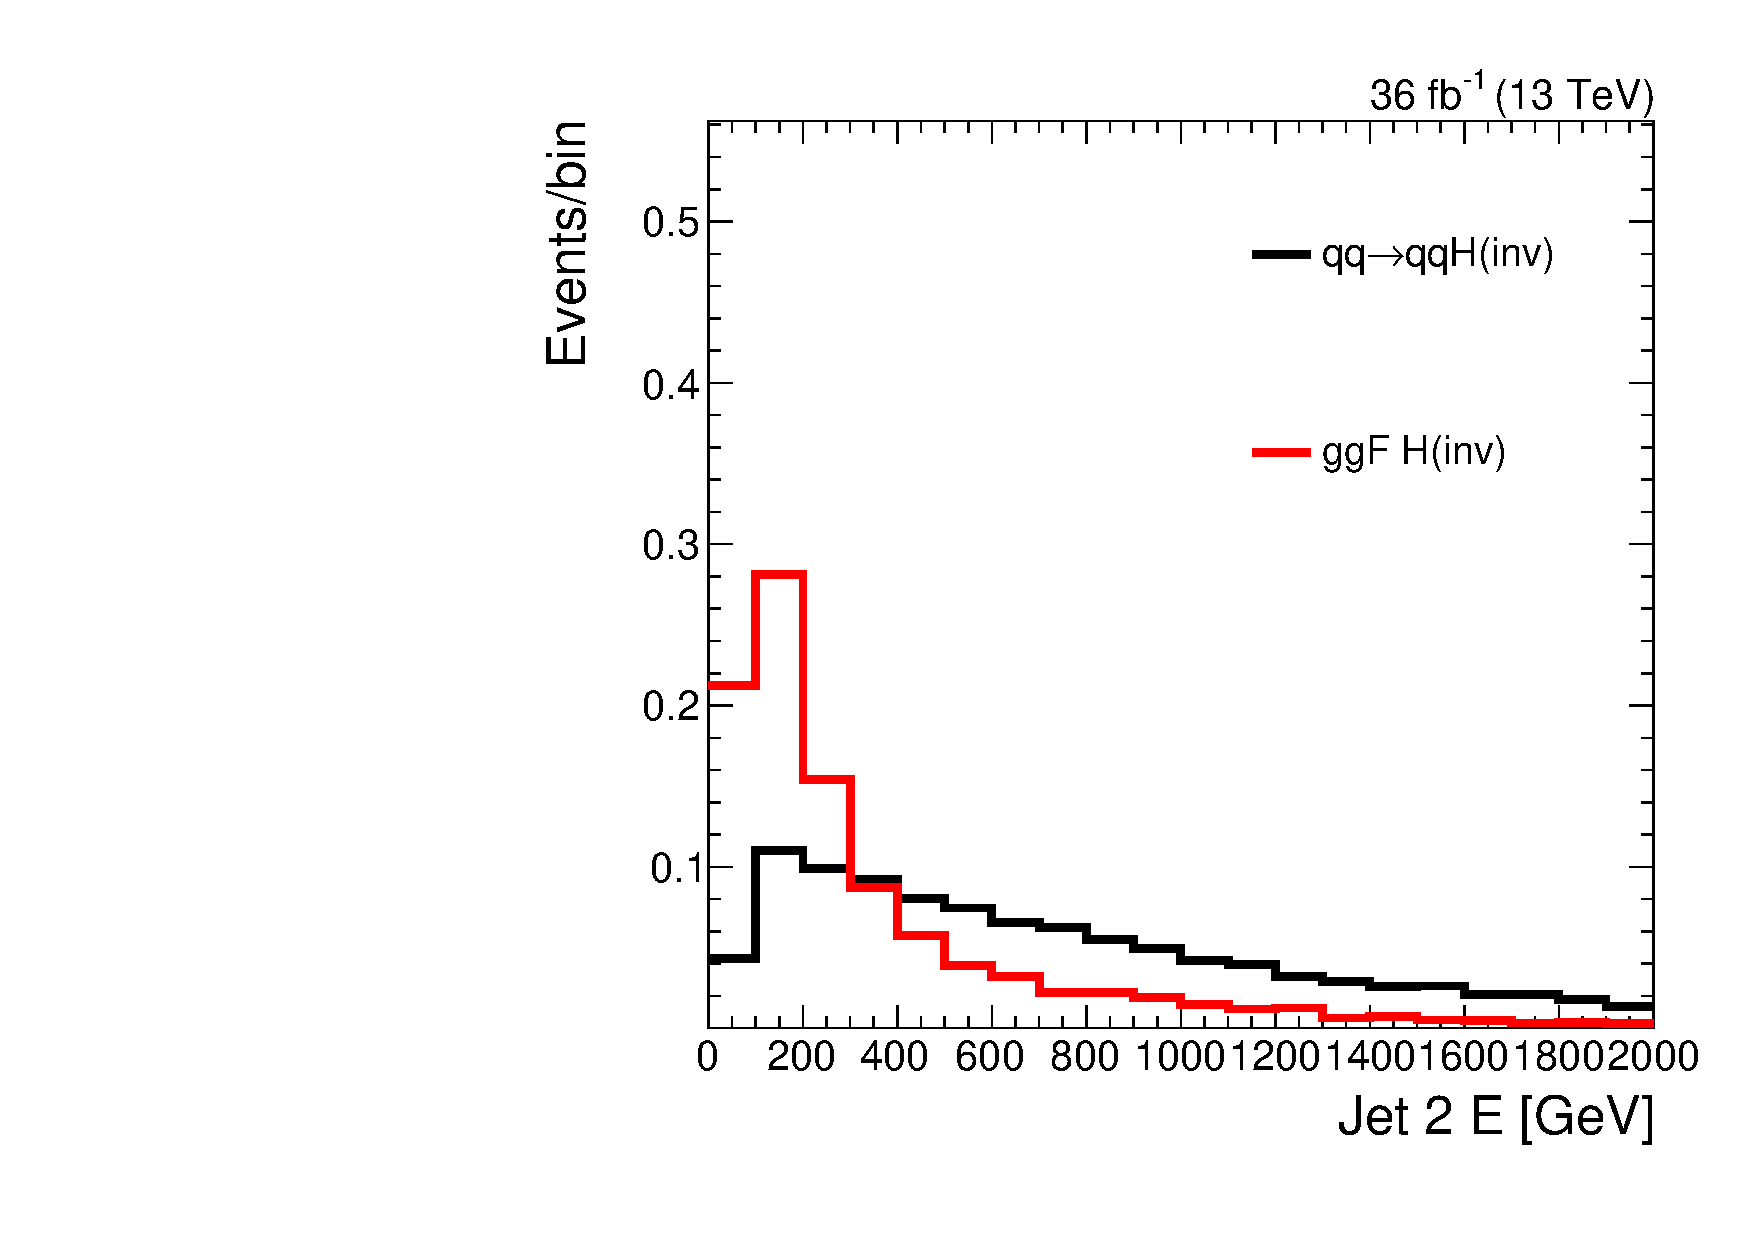
\includegraphics[width=0.32\textwidth]{figures/vbf/shapes_signal/loosesignal_jotE_1_.pdf} 
        \caption{Jet distributions, as compared between VBF and gluon fusion production modes.
                 A threshold is placed on the Higgs \pt~  by requiring $\ptmiss>250$ GeV.
                 Gluon fusion jets are typically from ISR or from the fermion loop; thus they do not exhibit the characteristic signatures of VBF jets.}
        \label{fig:vbf:sigkins}
    \end{center}
\end{figure}

\subsection{Online trigger selection}
\label{sec:vbf:trig}

The same trigger decisions (L1 and HLT) as described in Section~\ref{sec:mt:trigger} are used to select events in this analysis.
However, the L1 seeds for the 2016 data run were designed with mono-top-like analyses in mind; i.e., searches where the momentum imbalance is created by central objects.
To avoid noise and resolution issues in the forward calorimeters, the L1 seed only considers energy deposits in the region ${|\eta|<3}$. 
Therefore, VBF events in which both jets are in the forward region are not selected.  

This is visible in Figure~\ref{fig:vbf:hlta}, where events are classified based on the location of the two highest-$\pt$ jets.
Events with both jets in the barrel (BB) have a higher efficiency than events with one jet in the forward detector (BF).
Note that events with two forward jets (FF) are not considered at all, as the efficiency for such events is essentially zero. 

\begin{figure}[]
    \begin{center}
        \begin{subfigure}[t]{0.49\textwidth}
            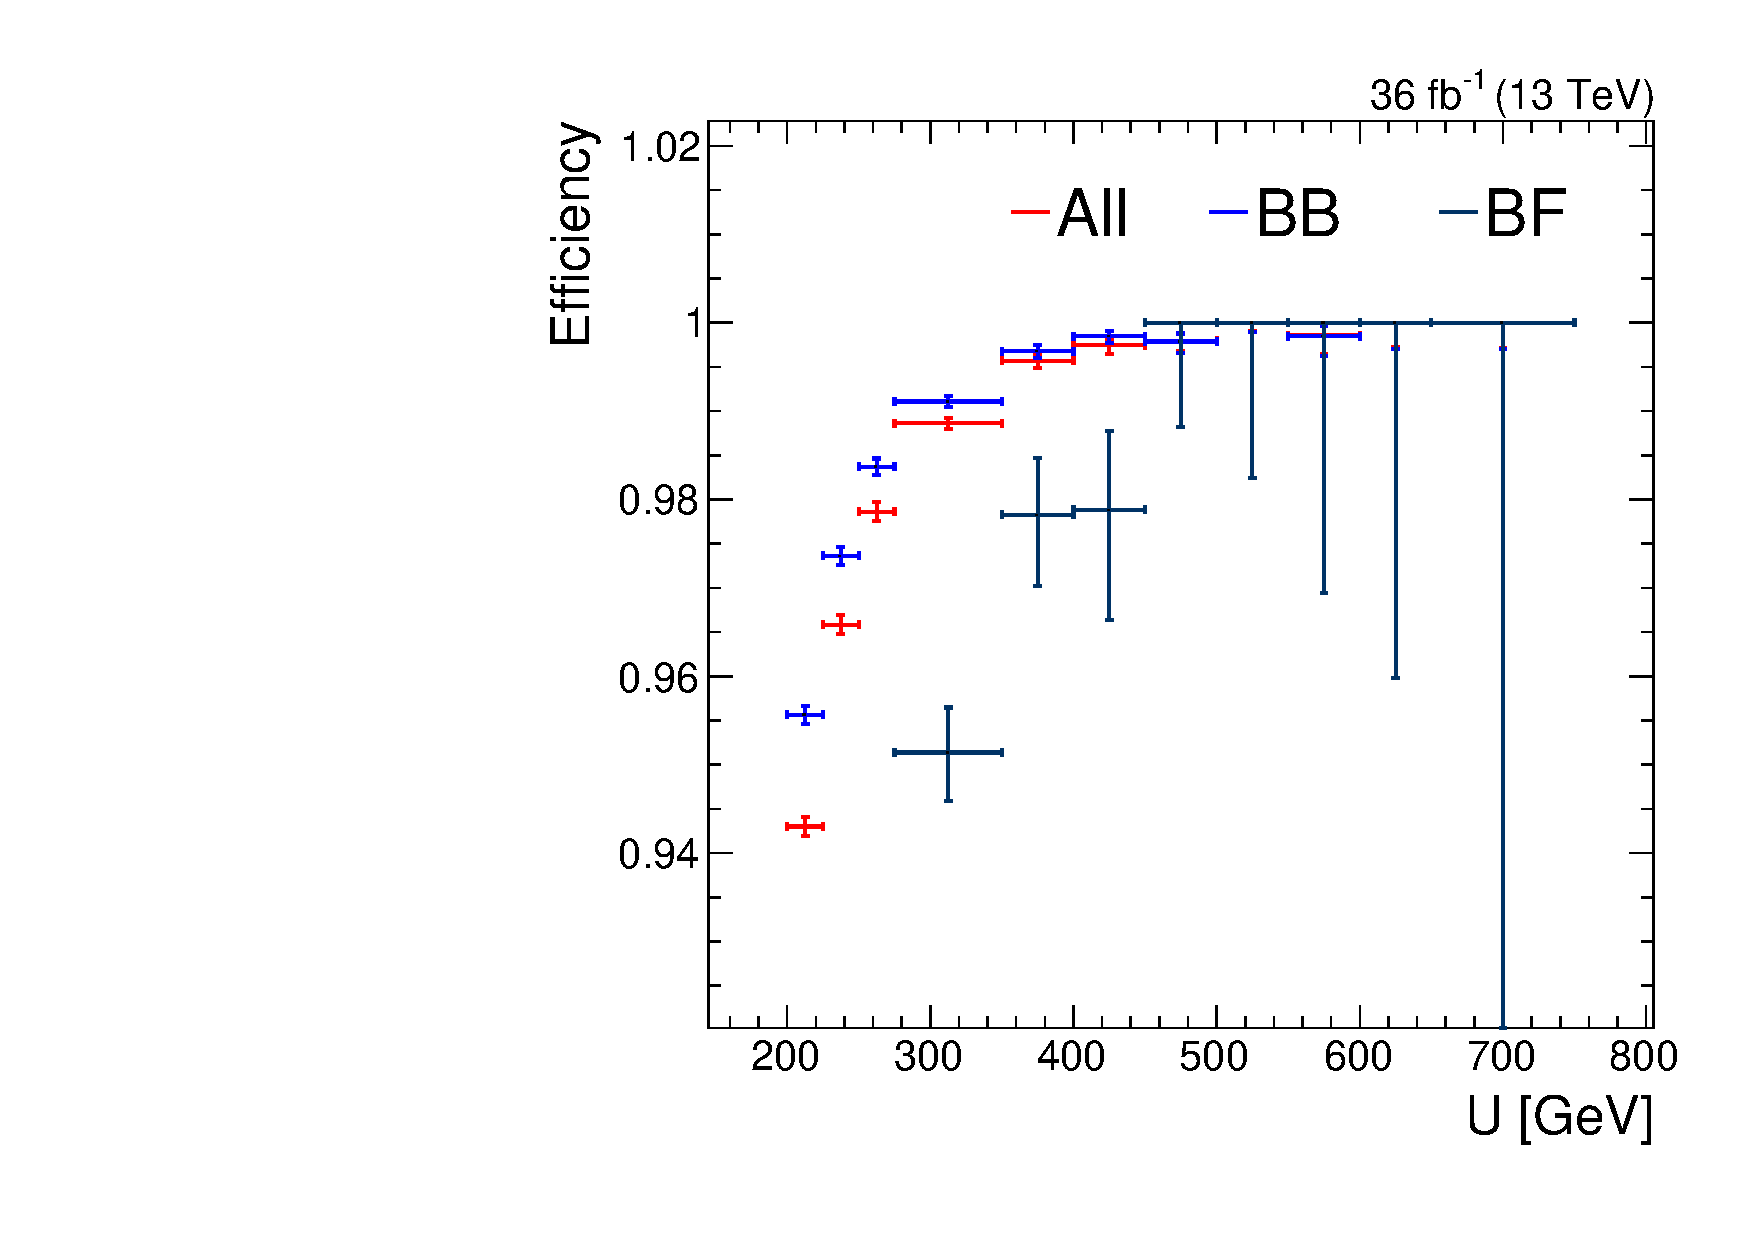
\includegraphics[width=\textwidth]{figures/vbf/triggers/trigeff_nmu1pfUWmag.pdf}
            \caption{Recoil}
            \label{fig:vbf:hlta}
        \end{subfigure}
        \begin{subfigure}[t]{0.49\textwidth}
            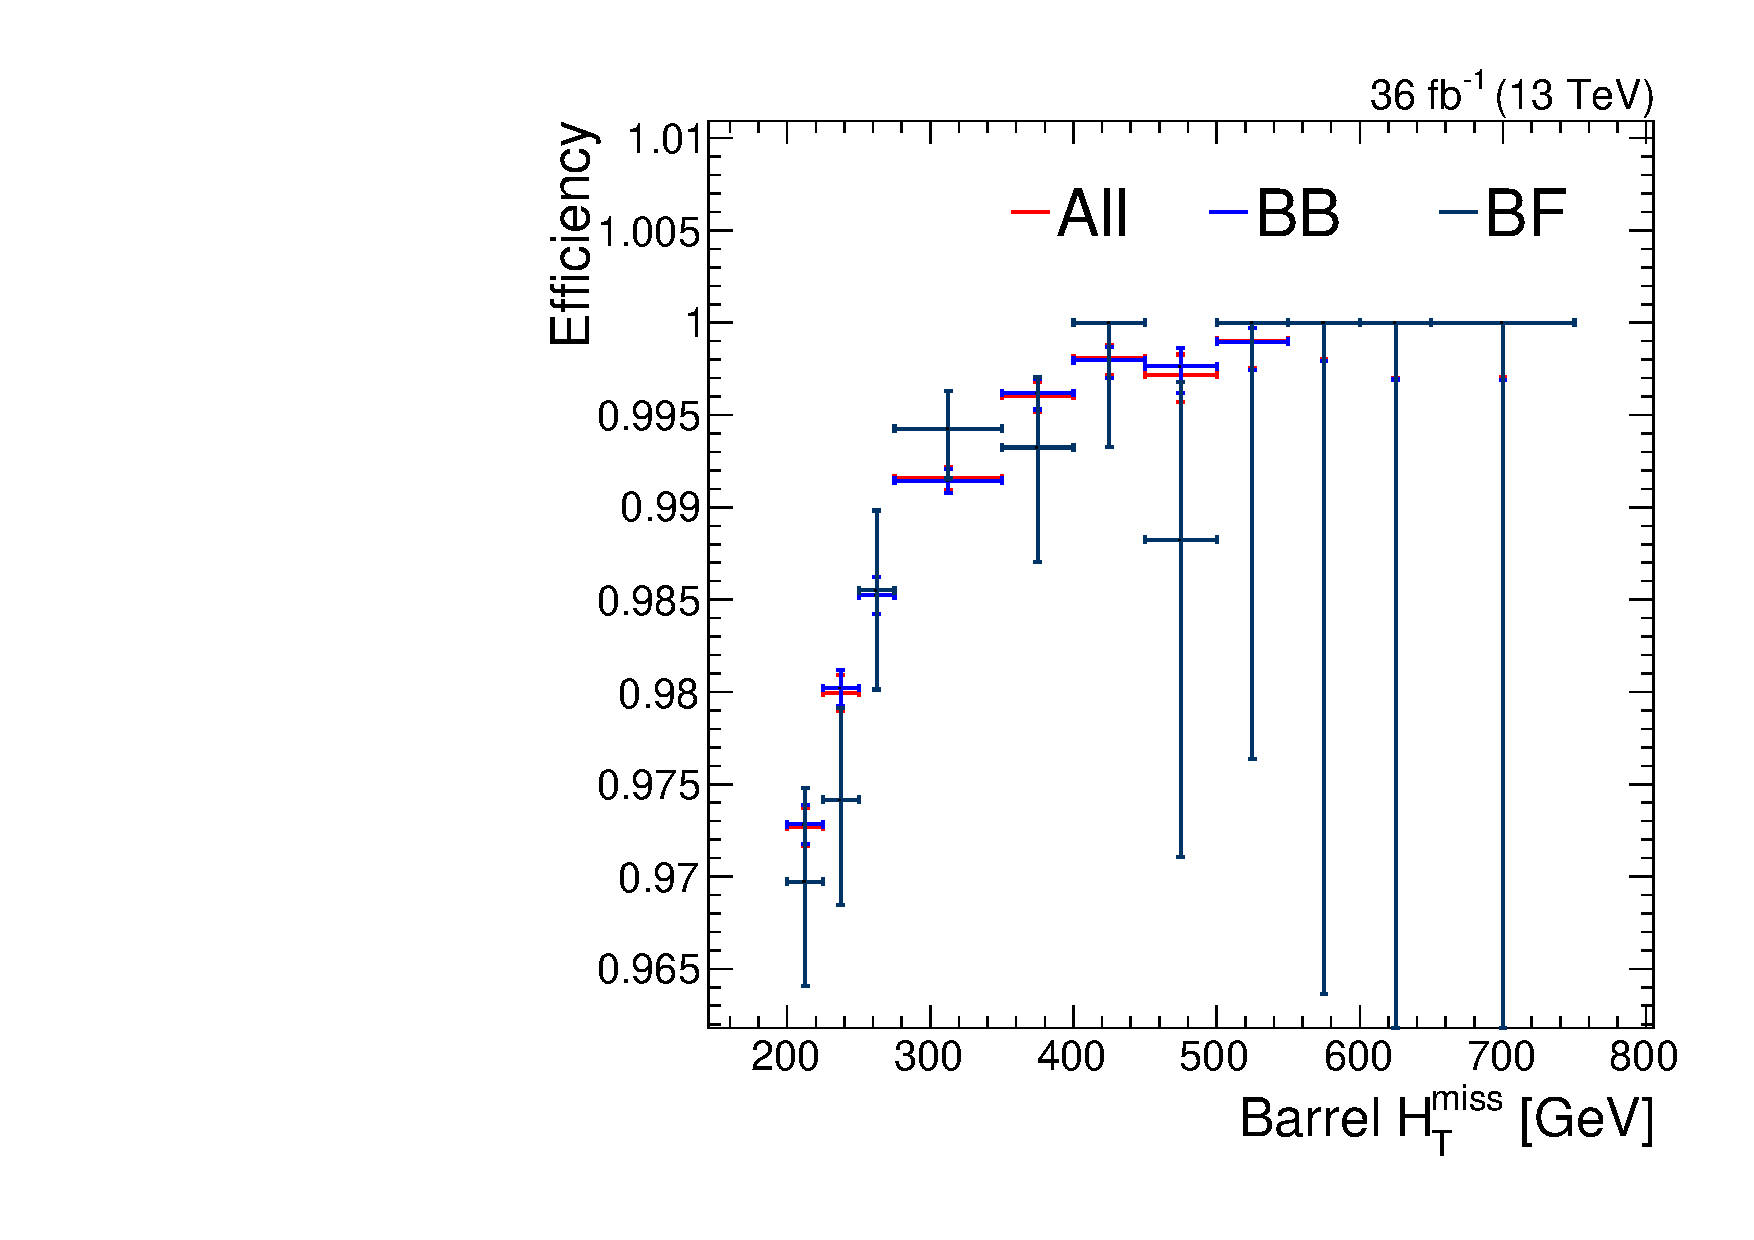
\includegraphics[width=\textwidth]{figures/vbf/triggers/trigeff_nmu1barrelHTMiss.pdf}
            \caption{$H_\mathrm{T,barrel}^\mathrm{miss}$}
            \label{fig:vbf:hltb}
        \end{subfigure}
        \caption{Trigger efficiency of events with a VBF-like topology (two jets with $\pt>80,40$ GeV) as a function of two different observables.
                 Events are split into two categories: those where both jets have $|\eta|<3$ (BB) and those where exactly one jet has $|\eta|>3$ (BF).
                 ``All'' refers to the sum of these categories.}
        \label{fig:vbf:hlt}
    \end{center}
\end{figure}

The trigger efficiency is truly characterized by the energy deposited in the $|\eta|<3$ region of the detector, and will be dominated in VBF events by the energy of jets.
Accordingly, we define the \emph{missing barrel hadronic transverse momentum}:
\begin{equation}
    H_\mathrm{T,barrel}^\mathrm{miss} = \left|\left(\sum_{j\in\text{barrel}} \vec{p}_j \right)_\mathrm{T}\right|, \text{ where barrel refers to jets with $|\eta|<3$}
\end{equation}
As shown in Figure~\ref{fig:vbf:hltb}, the three categories (BB, BF, All) have similar behavior as a function of $H_\mathrm{T,barrel}^\mathrm{miss}$.
Therefore, we use this parameterization of the efficiency to correct MC simulation to match data. 

A second L1-related issue that plagues the 2016 dataset is the \emph{pre-firing} effect.
This occurs when an ECAL deposit in a particular bunch crossing (\bx{0}) is mis-timed by the L1, leading the ECAL cluster to be assigned to the previous event (\bx{-1}).
If this anomalous cluster causes the L1 to accept \bx{-1}, the L1 will not consider \bx{0}.
The portion of the ECAL covering $2.5 < |\eta| < 3$ is particularly prone to this issue.
As VBF jets frequently deposit energy in this region, it must be corrected for. 
Details of the pre-firing mechanism and the derivation of the correction are provided in Appendix~\ref{sec:prefire}.
An unbiased sample of muon-triggered events are used to determine the probability of a pre-fire $\epsilon(\bx{-1})$.
This sample is statistically limited, so it is supplemented by a jet-triggered measurement.
Although jet-based triggers have a weak correlation with $\epsilon(\bx{-1})$, this is at low jet $\pt$, where the muon-triggered measurement is sufficient. 
The resulting probabilities are shown in Figure~\ref{fig:vbf:pre_eff2_pteta1} and are applied to the MC as a function of jet \pt~ and $\eta$.
A relative 20\% uncertainty is assessed on the efficiency, which is derived from the difference between the muon and jet measurements. 

\begin{figure}[]
    \begin{center}
        \begin{subfigure}[t]{0.49\textwidth}
            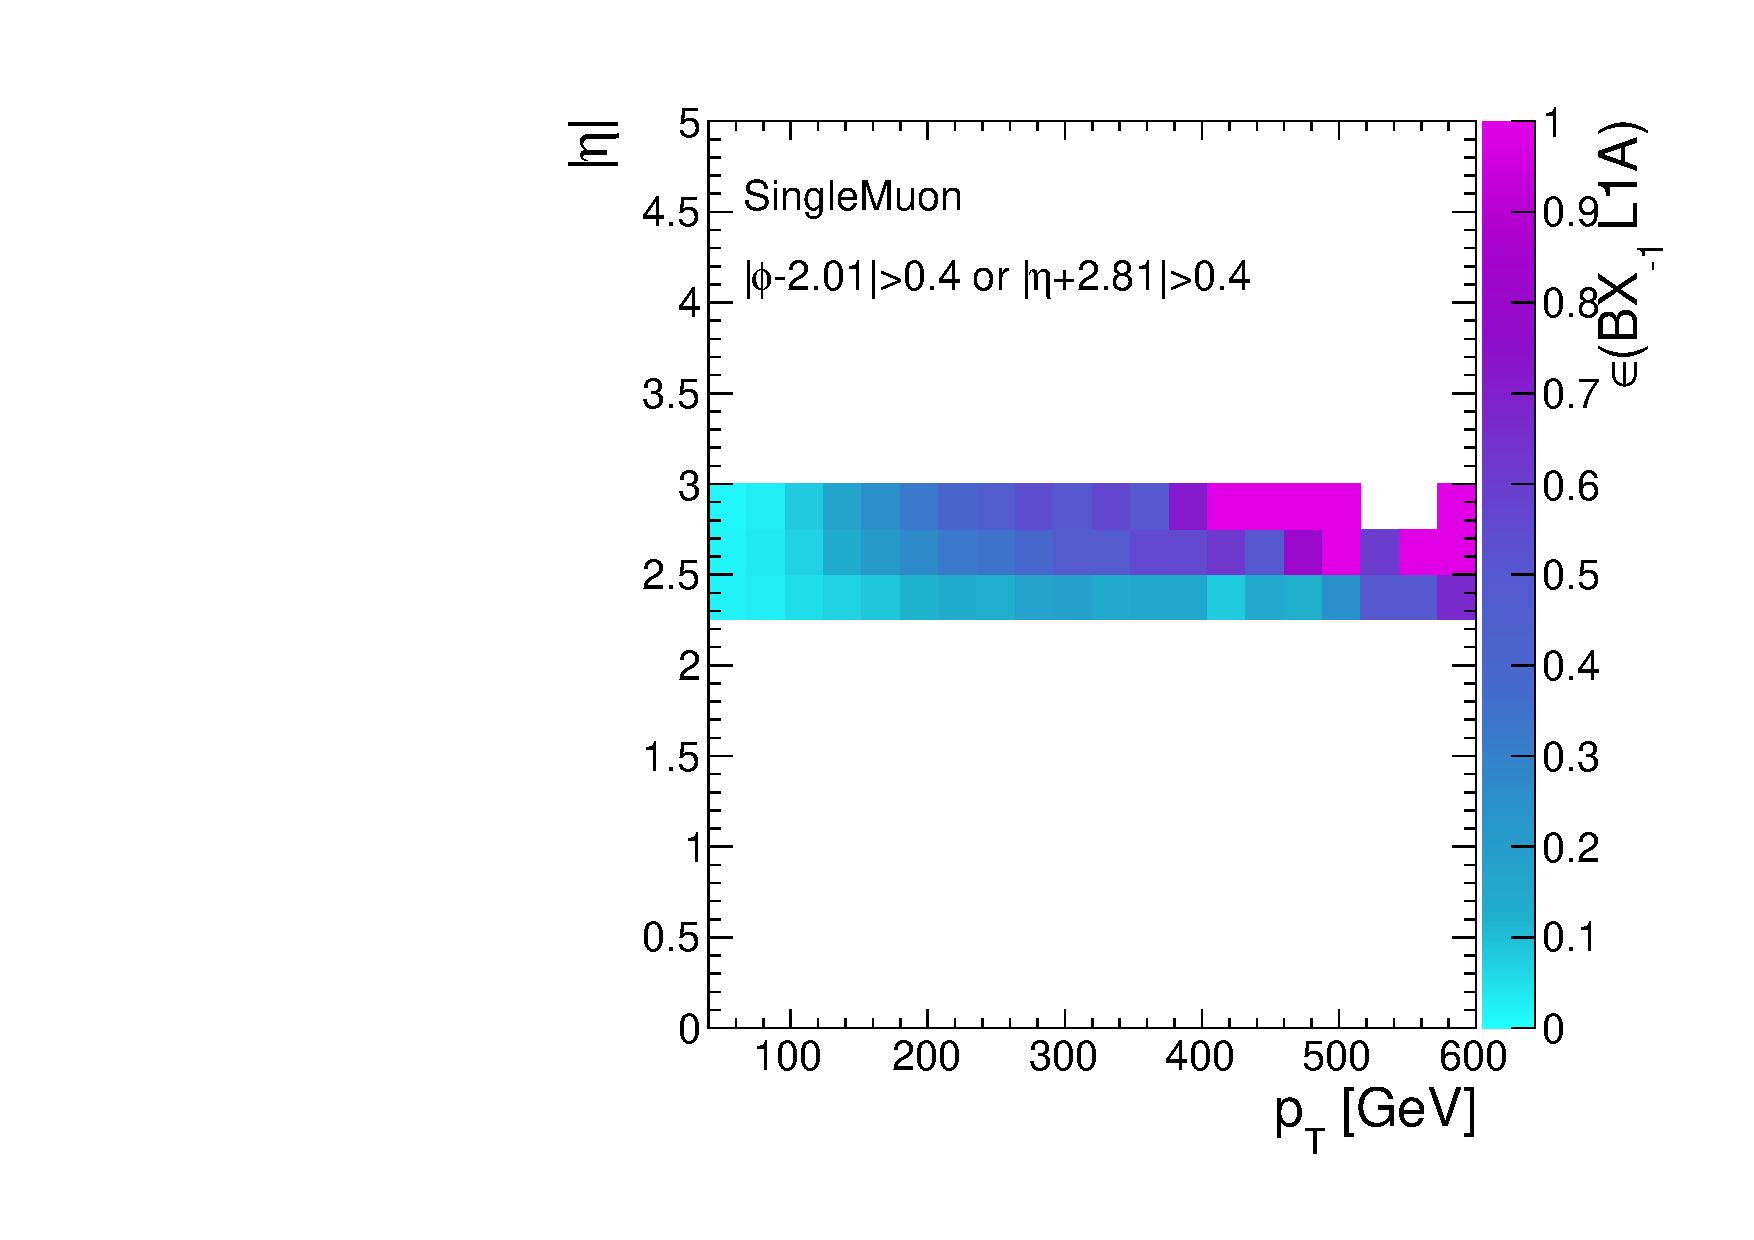
\includegraphics[width=\textwidth]{figures/vbf/triggers/SingleMuon_spike_finor_pteta_ratio.pdf}
            \caption{Muon-triggered}
        \end{subfigure}
        \begin{subfigure}[t]{0.49\textwidth}
            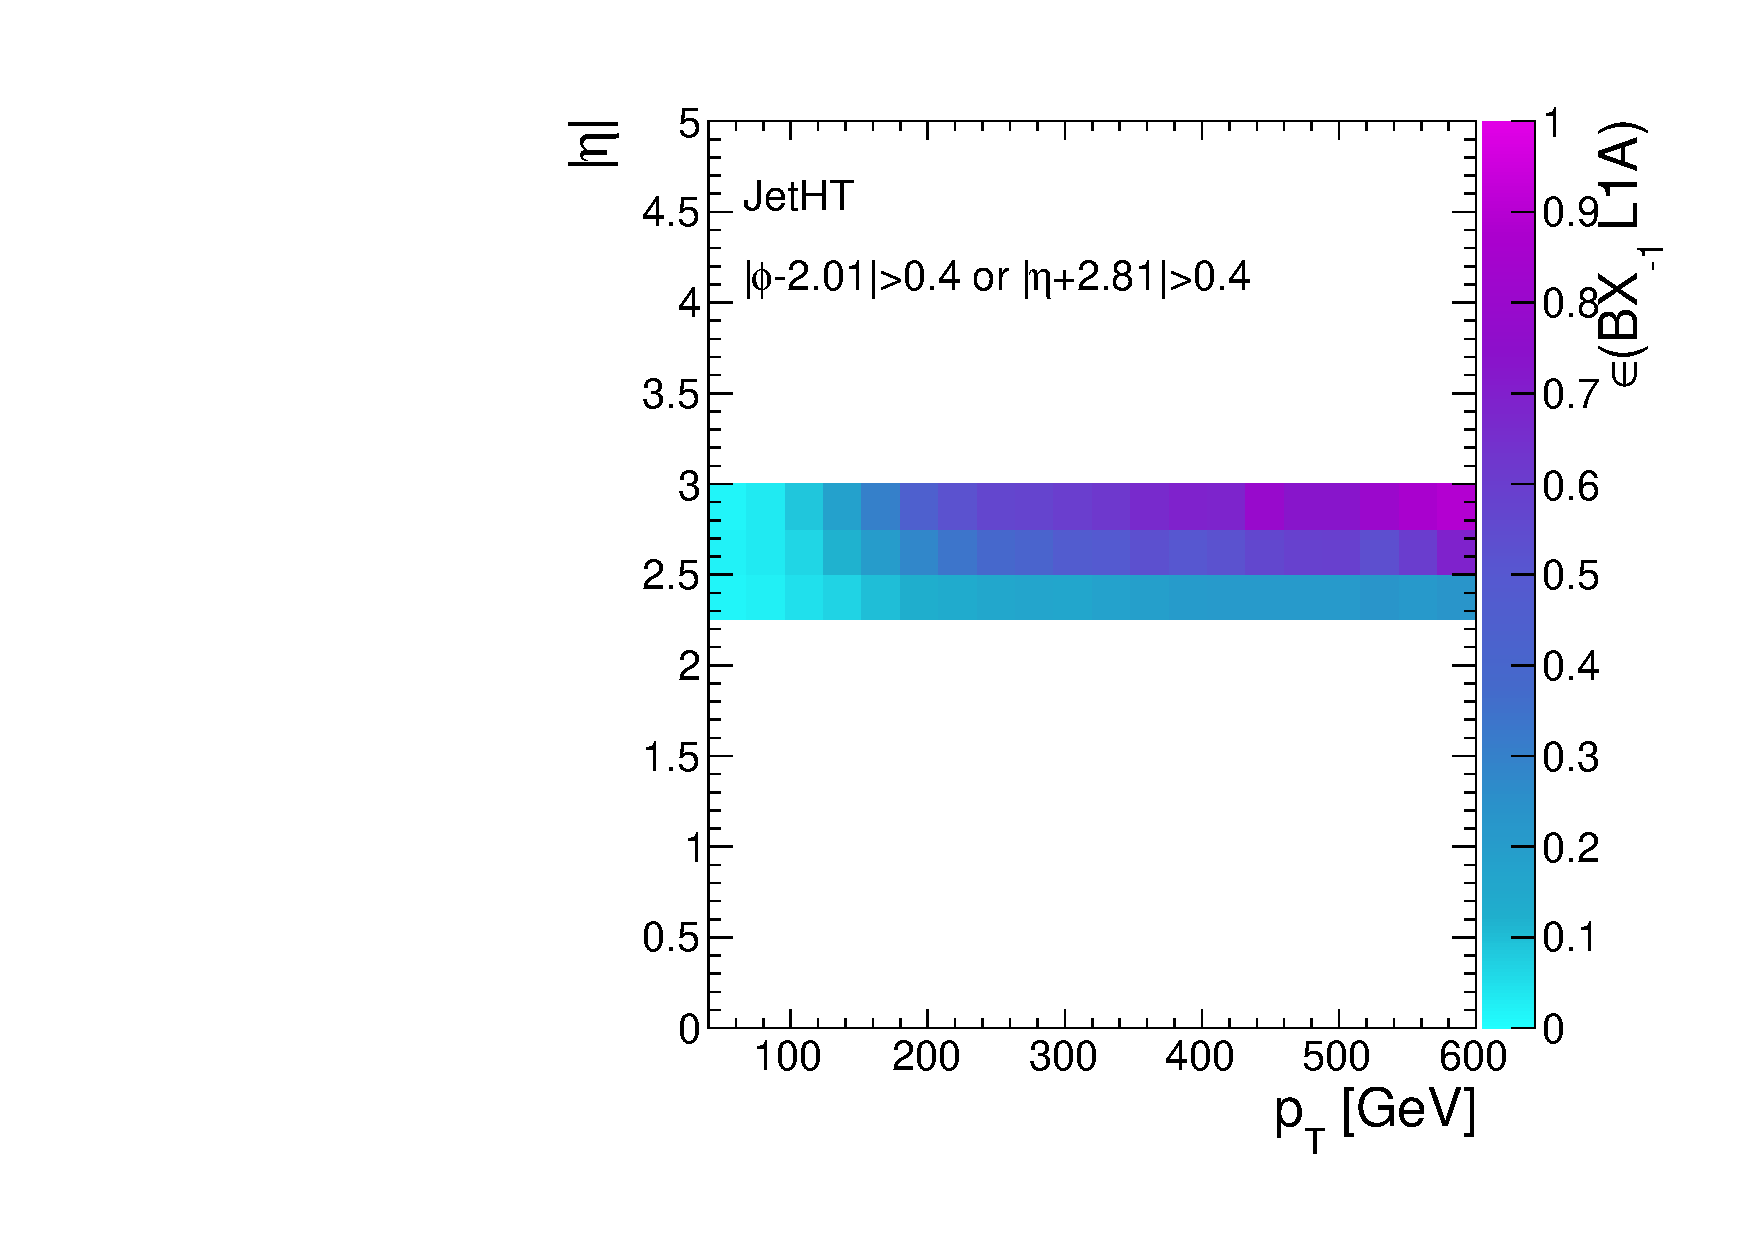
\includegraphics[width=\textwidth]{figures/vbf/triggers/JetHT_spike_finor_pteta_ratio.pdf}
            \caption{Jet-triggered}
        \end{subfigure}
        \caption{$\epsilon_\text{pre-fire}(\pt,\eta)$ with two different sets of reference triggers used to select \bx{0}.
                 Muon-triggered events are used below $250$ GeV, to minimize the bias from jet triggers.
                 Jet-triggered events are used above this threshold, to minimize the statistical uncertainty.}
        \label{fig:vbf:pre_eff2_pteta1}
    \end{center}
\end{figure}

\subsection{EW and QCD production of electroweak bosons}

The primary backgrounds to the VBF production of invisibly-decaying Higgs bosons are $Z(\rightarrow\nu\nu)$+2 jet and $W(\rightarrow\ell\nu)$+2 jet production.
At leading order, the relevant Feynman diagrams are either of the order $\alpha_\mathrm{EW}^2 \alpha_\mathrm{QCD}^4$ or $\alpha_\mathrm{EW}^6$. 
We refer to the former as the QCD production mode and the latter as the EW mode. 
Examples Feynman diagrams are shown in Figure~\ref{fig:vbf:ewqcd}.
The EW mode is essentially vector boson fusion, and so the terms EW and VBF will be used interchangeably. 


\begin{figure}[]
    \begin{center}
        \begin{subfigure}[t]{0.49\textwidth}
            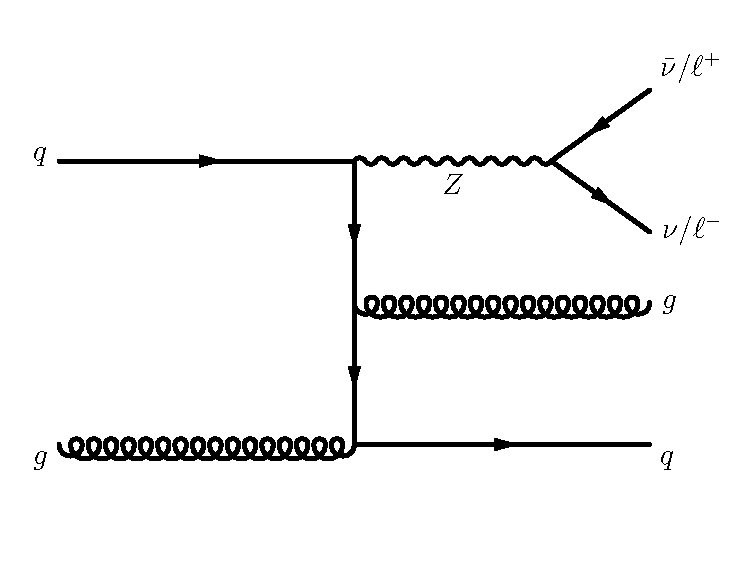
\includegraphics[width=\textwidth]{figures/vbf/diagrams/qcd_z.pdf}
            \caption{QCD}
        \end{subfigure}
        \begin{subfigure}[t]{0.49\textwidth}
            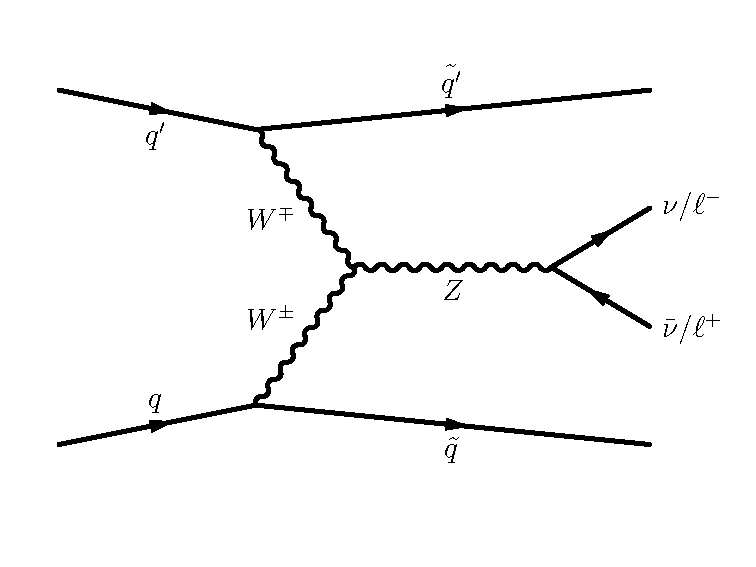
\includegraphics[width=\textwidth]{figures/vbf/diagrams/vbf_z.pdf}
            \caption{EW/VBF}
        \end{subfigure}
        \caption{Examples of the two modes of producing $Z$ bosons in association with 2 jets.
                 Similar diagrams exist for $W$ boson production.}
        \label{fig:vbf:ewqcd}
    \end{center}
\end{figure}

As the vector boson is not directly detectable, the only experimental signatures are the jets.
The jet kinematics are sensitive to the production mode (vector boson fusion vs QCD), as well as the spin of the produced boson.
Some conclusions can be drawn from the kinematic distributions (Figure~\ref{fig:vbf:jetkins}):
\begin{enumerate}
    \item The yield ($\sigma\times A$) of the three VBF processes are relatively close in the relevant phase space (assuming $\mathcal{B}(\hinv)=1$), but the QCD processes are 1-2 orders of magnitude higher.
    \item The jet $\pt$ and $\ptmiss$ distributions in the signal are comparable to or softer than the background processes. 
          This is in contrast to other DM searches, in which the signal $\ptmiss$ distribution is much harder than SM predictions.
    \item VBF $\hinv$ produces fewer jets than SM processes.
    \item VBF $\hinv$ produces relatively forward jets. QCD $V$+jets produces mostly central jets. EW $V$+jets produces jets in an intermediate range. 
\end{enumerate}

\begin{figure}[]
    \begin{center}
        \begin{subfigure}[t]{0.32\textwidth}
            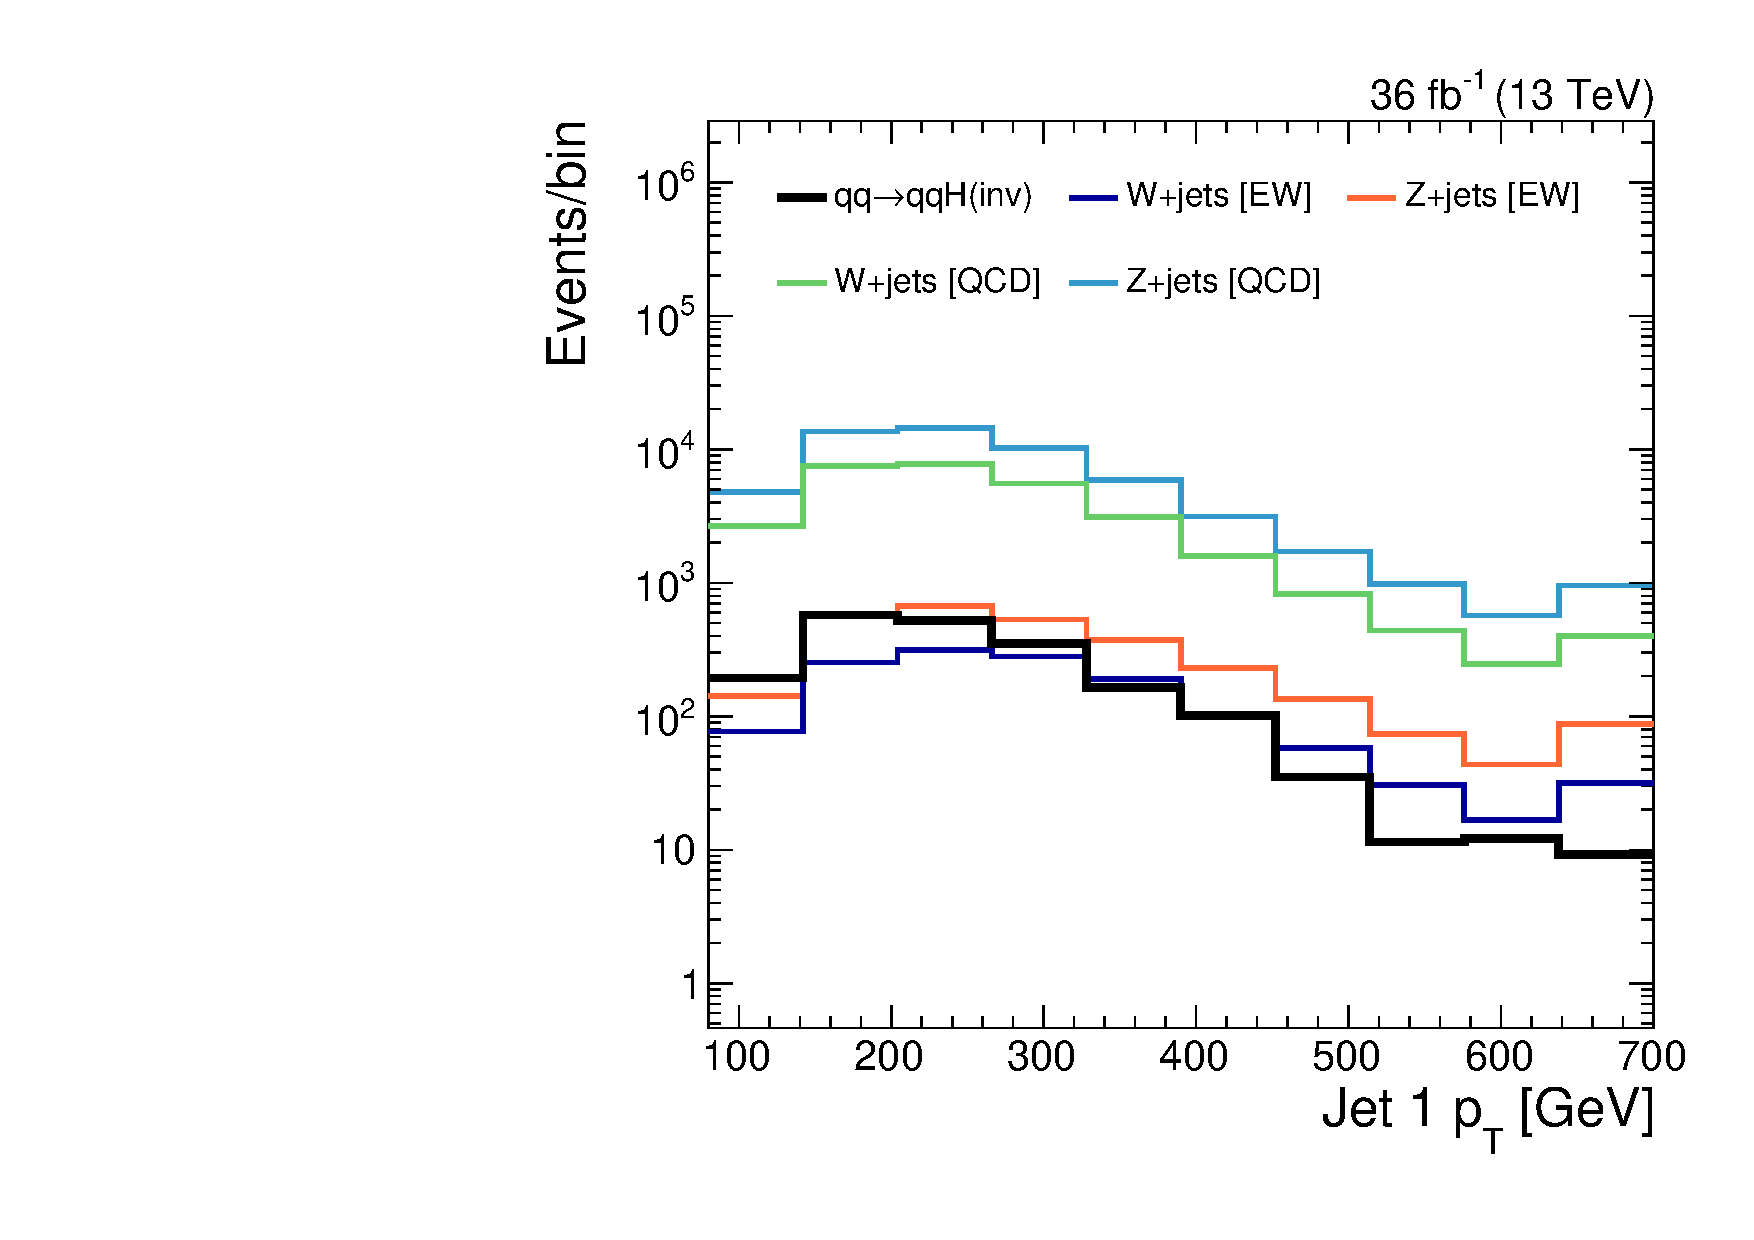
\includegraphics[width=\textwidth]{figures/vbf/shapes/loosesignal_jotPt_0__logy.pdf}
            \caption{Leading jet $\pt$}
        \end{subfigure}
        \begin{subfigure}[t]{0.32\textwidth}
            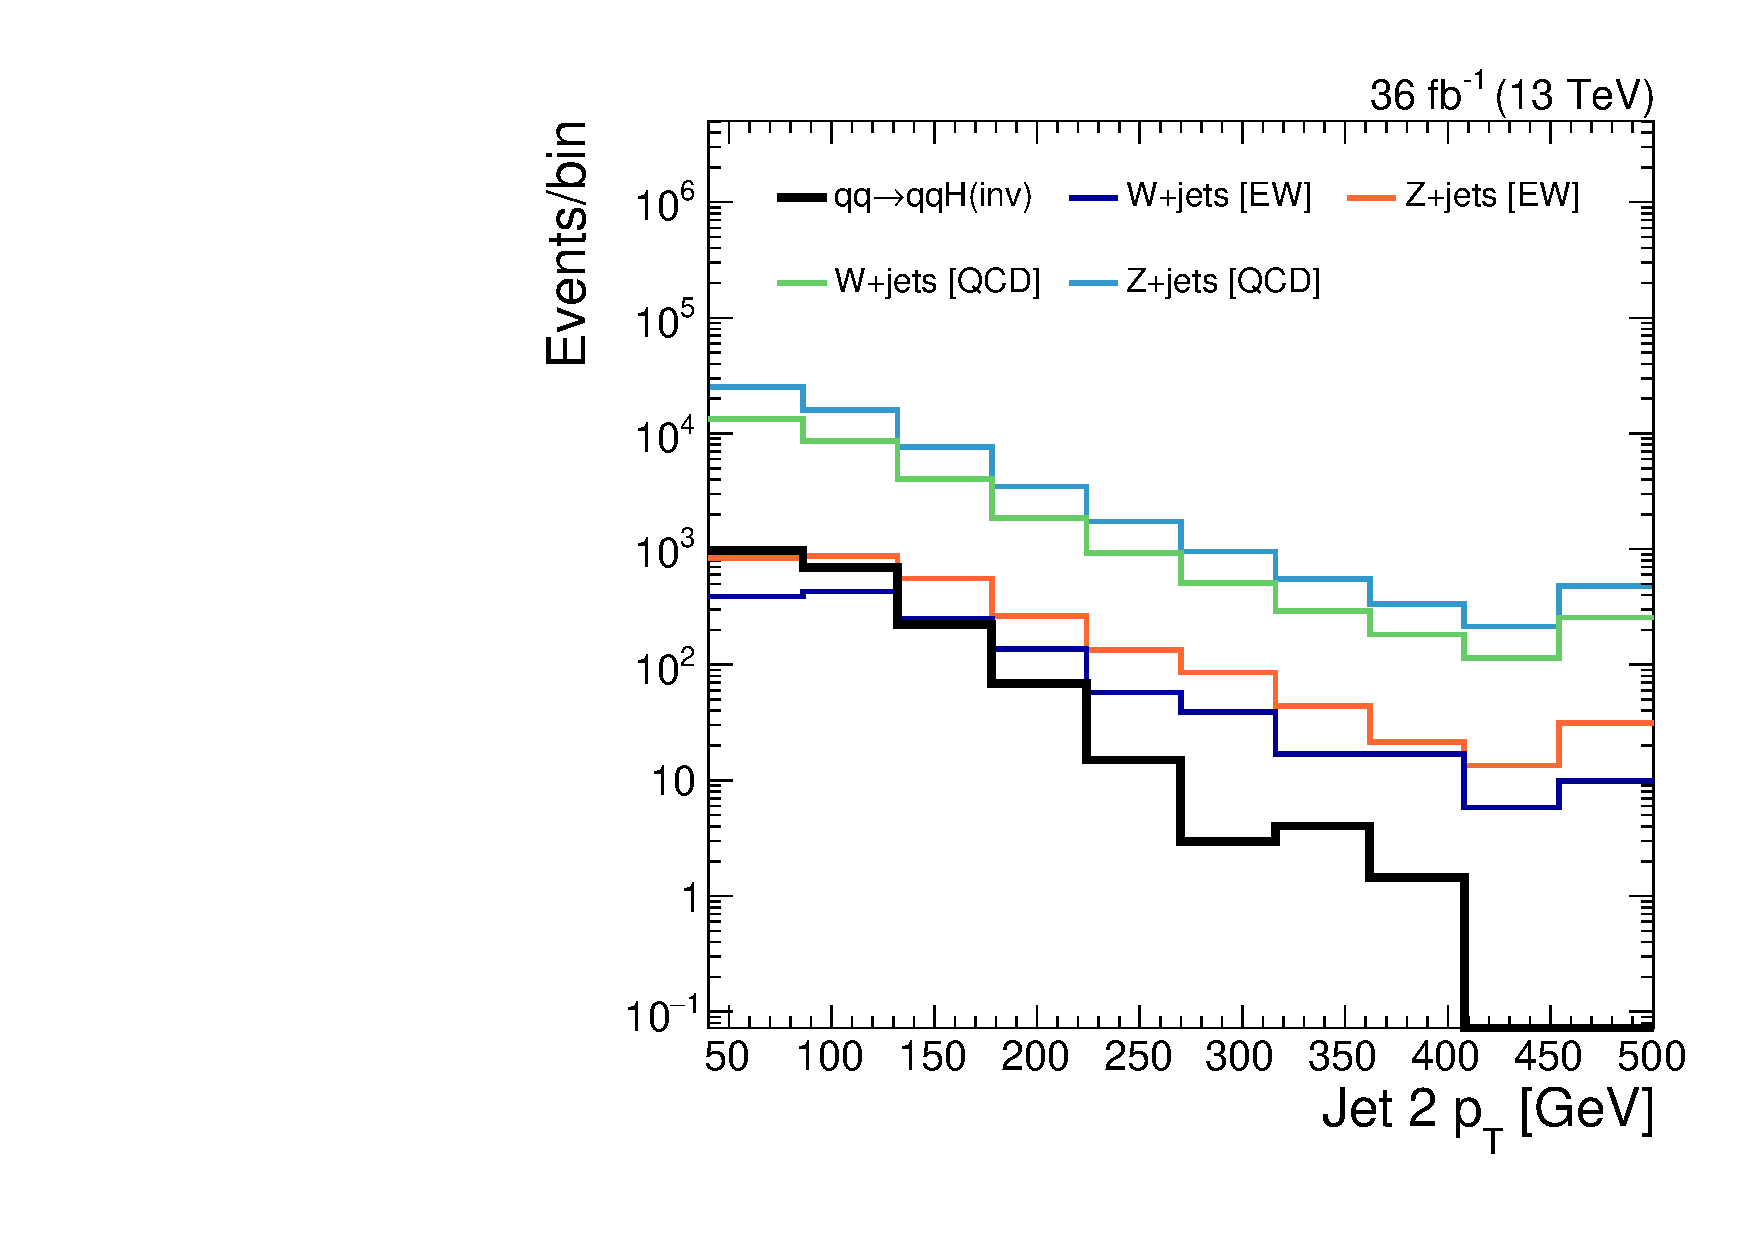
\includegraphics[width=\textwidth]{figures/vbf/shapes/loosesignal_jotPt_1__logy.pdf}
            \caption{Sub-leading jet $\pt$}
        \end{subfigure}
        \begin{subfigure}[t]{0.32\textwidth}
            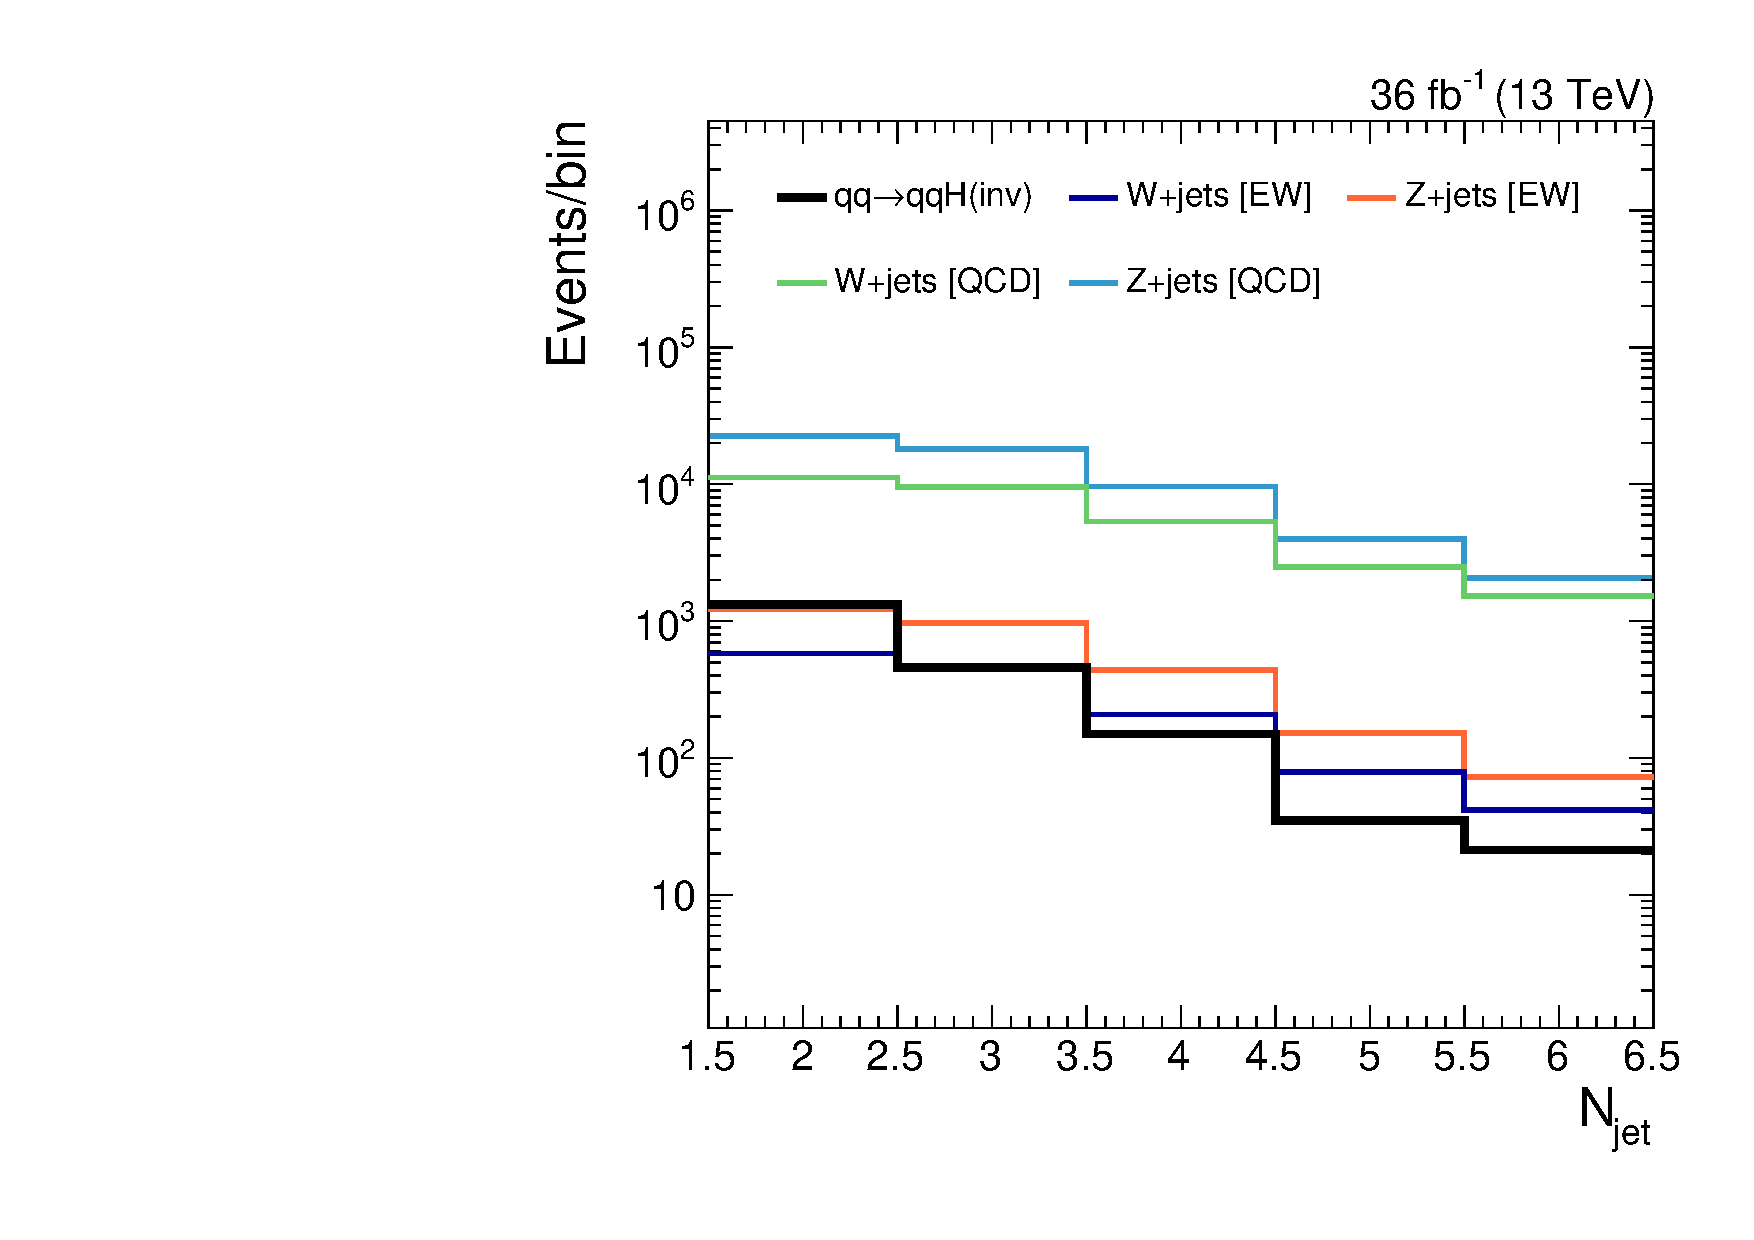
\includegraphics[width=\textwidth]{figures/vbf/shapes/loosesignal_nJot_logy.pdf}
            \caption{$N_\mathrm{jet}$}
        \end{subfigure}
        \begin{subfigure}[t]{0.32\textwidth}
            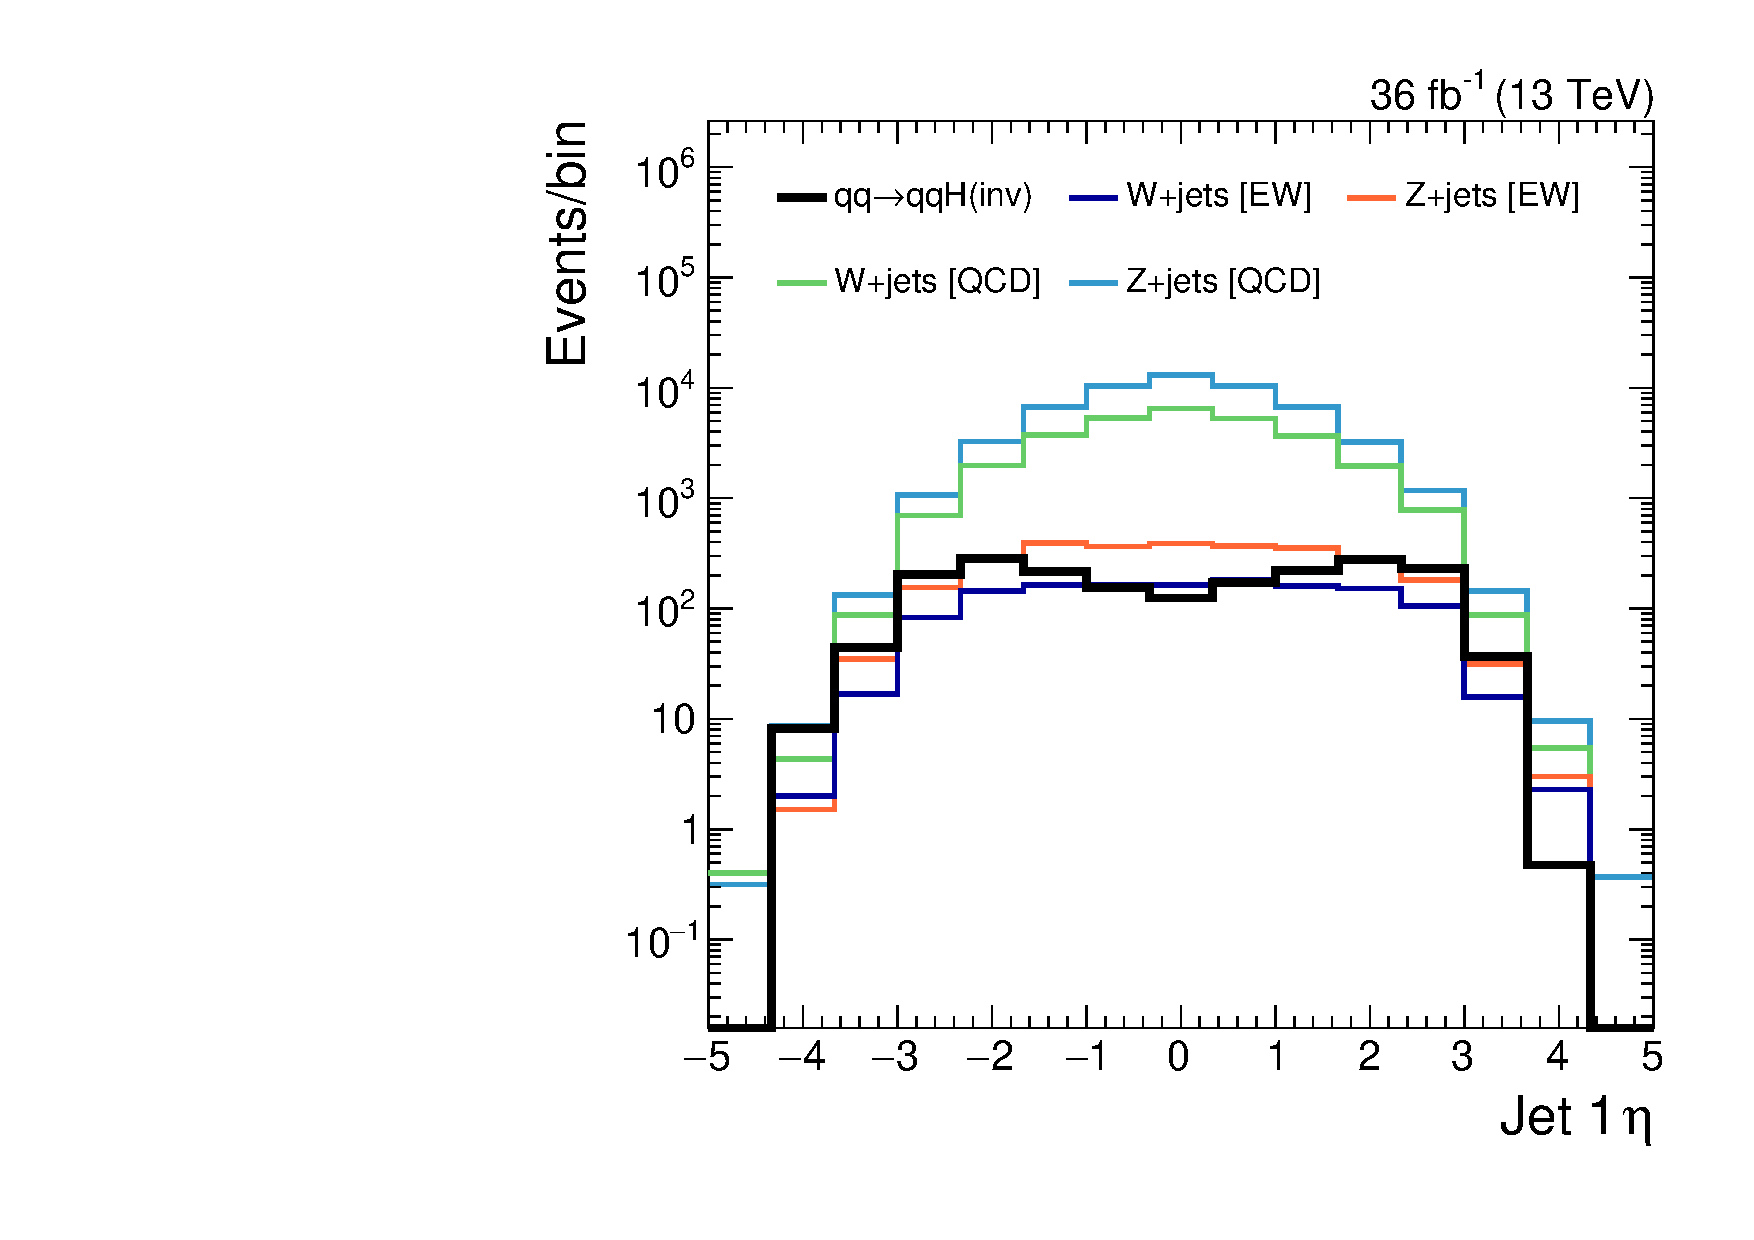
\includegraphics[width=\textwidth]{figures/vbf/shapes/loosesignal_jotEta_0__logy.pdf}
            \caption{Leading jet $\eta$}
        \end{subfigure}
        \begin{subfigure}[t]{0.32\textwidth}
            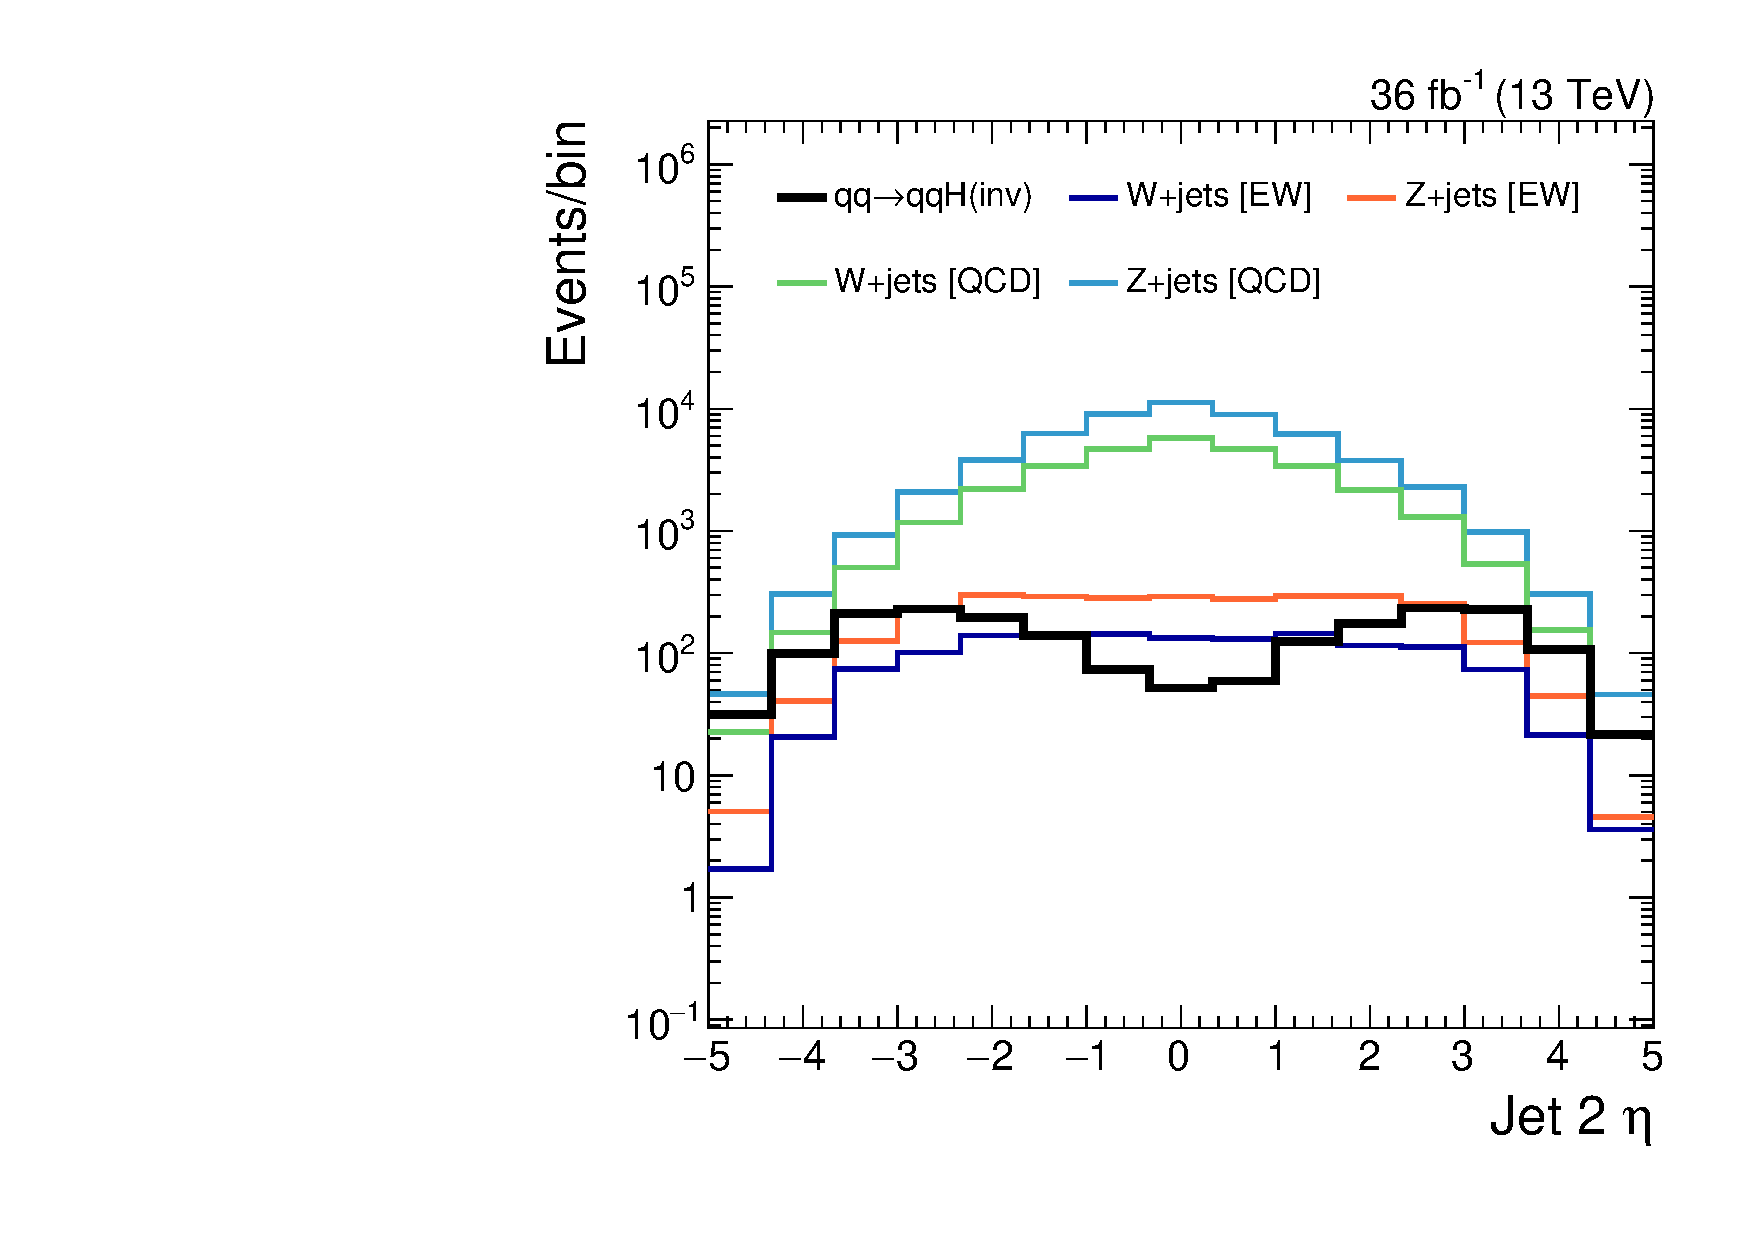
\includegraphics[width=\textwidth]{figures/vbf/shapes/loosesignal_jotEta_1__logy.pdf}
            \caption{Sub-leading jet $\eta$}
        \end{subfigure}
        \begin{subfigure}[t]{0.32\textwidth}
            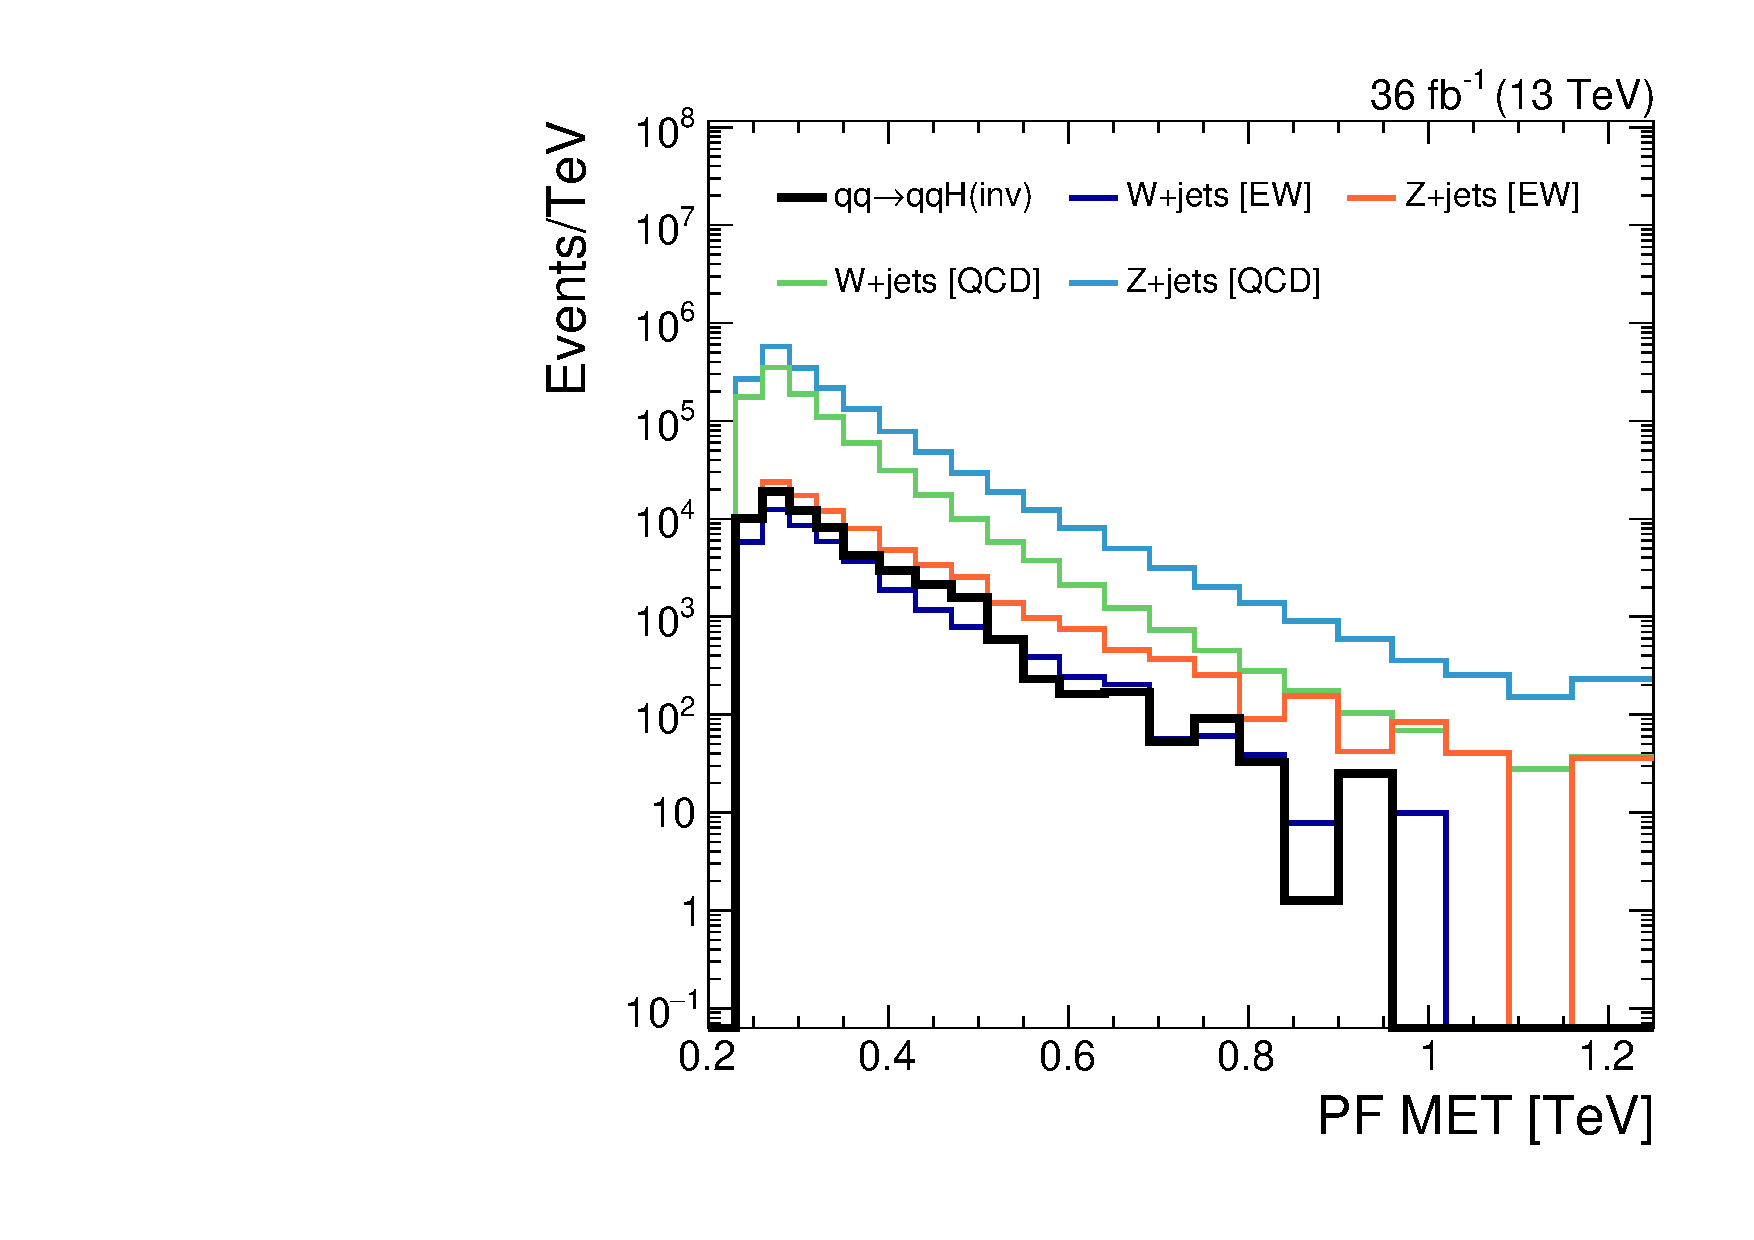
\includegraphics[width=\textwidth]{figures/vbf/shapes/loosesignal_pfmet_logy.pdf}
            \caption{$\ptmiss$}
        \end{subfigure}
        \caption{Event kinematic distributions, as compared between $H$ vs $Z$ vs $W$ production, and VBF vs QCD modes.}
        \label{fig:vbf:jetkins}
    \end{center}
\end{figure}

To fully exploit these kinematic distributions, we look at \emph{VBF-tag} observables, which are functions of the two leading jets. 
These are defined as:
\begin{itemize}
    \item[$m_{jj}$:] Invariant mass of the dijet system.
    \item[$\Delta\eta_{jj}$:] Absolute value of the difference in pseudorapidity of the two jets.
    \item[$\Delta\phi_{jj}$:] Absolute value of the difference in azimuthal angle of the two jets.
\end{itemize}
These distributions are shown in Figure~\ref{fig:vbf:dijetkins}.
The first two distributions look different in QCD and VBF processes and are therefore useful to reduce QCD backgrounds.
On the other hand, \dphi~is sensitive to the spin of the boson produced in a VBF process, and therefore can distinguish between Higgs and electroweak boson production.

\begin{figure}[]
    \begin{center}
        \begin{subfigure}[t]{0.32\textwidth}
            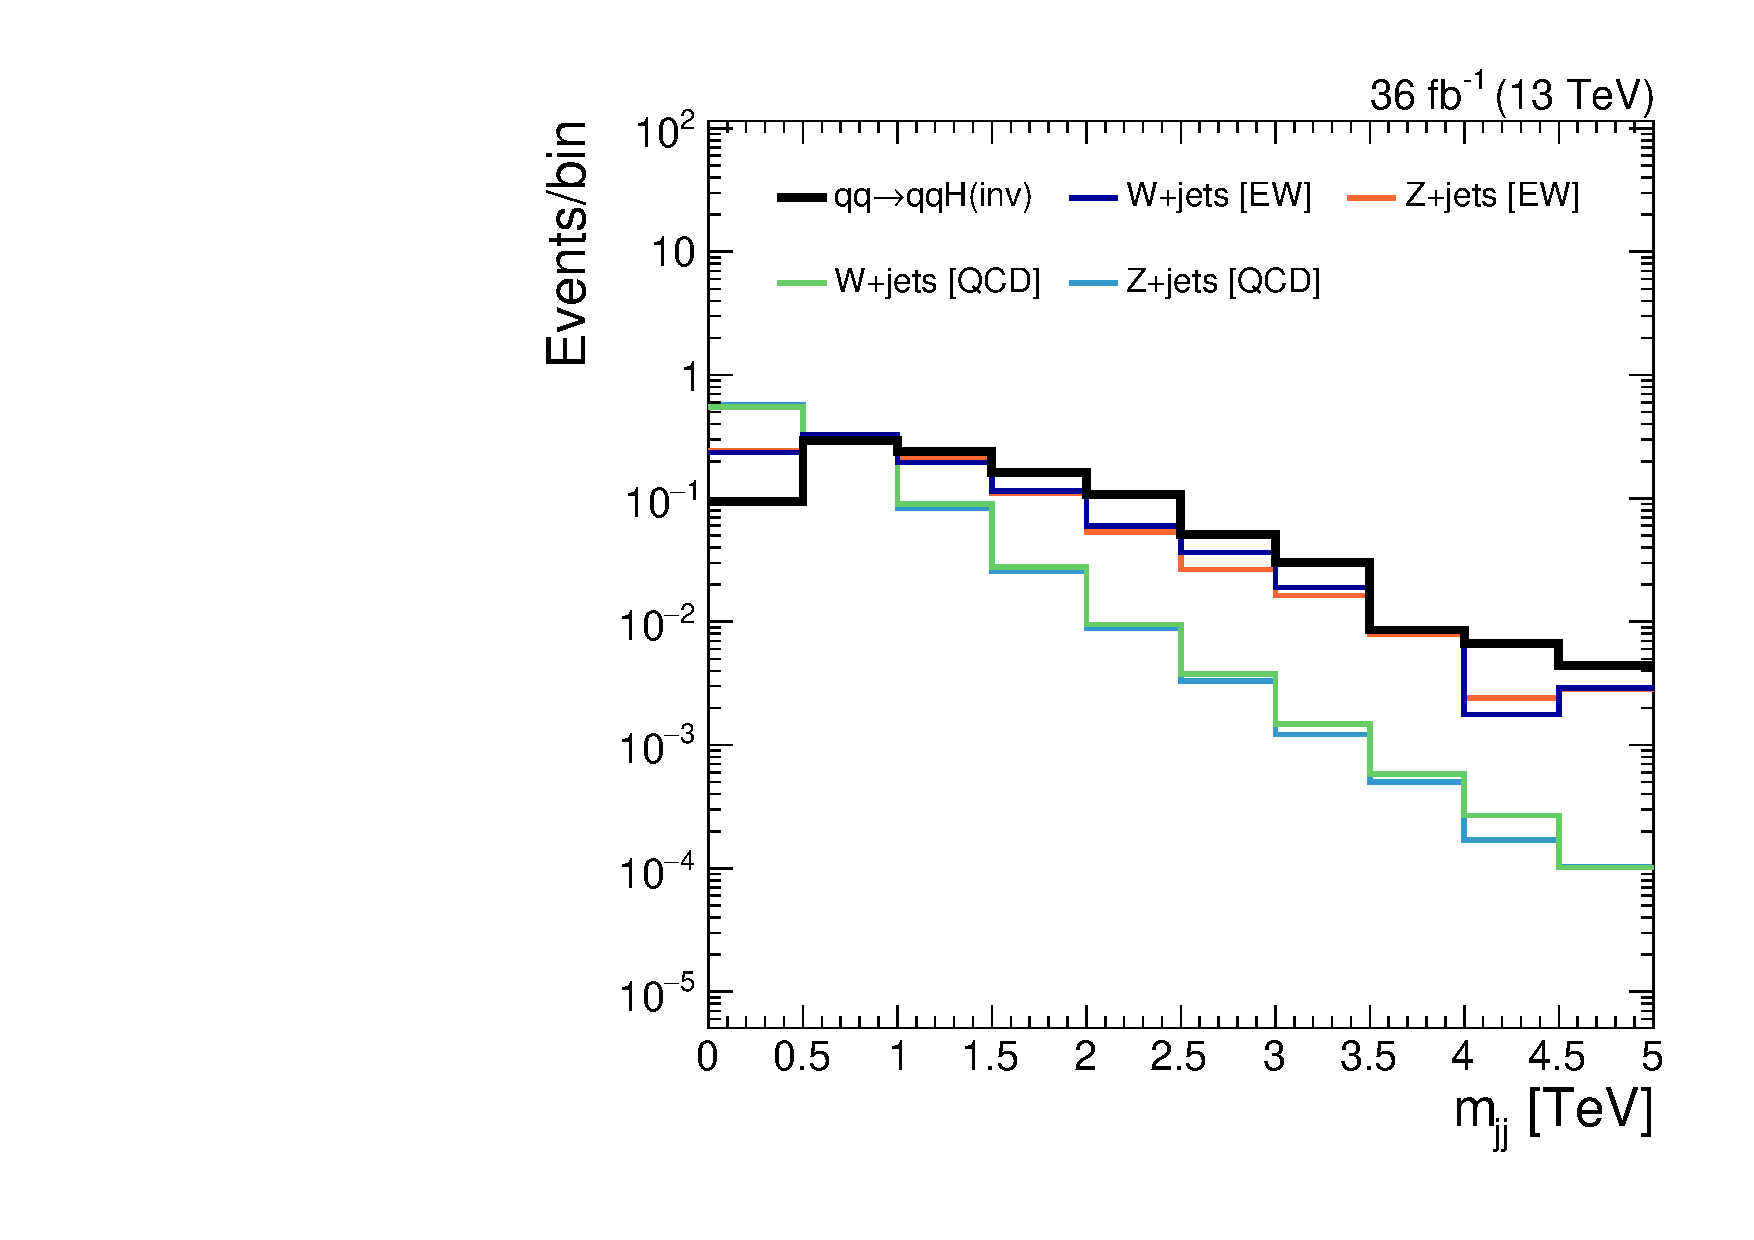
\includegraphics[width=\textwidth]{figures/vbf/shapes/loosesignal_jot12Mass_logy.pdf}
            \caption{\mjj}
        \end{subfigure}
        \begin{subfigure}[t]{0.32\textwidth}
            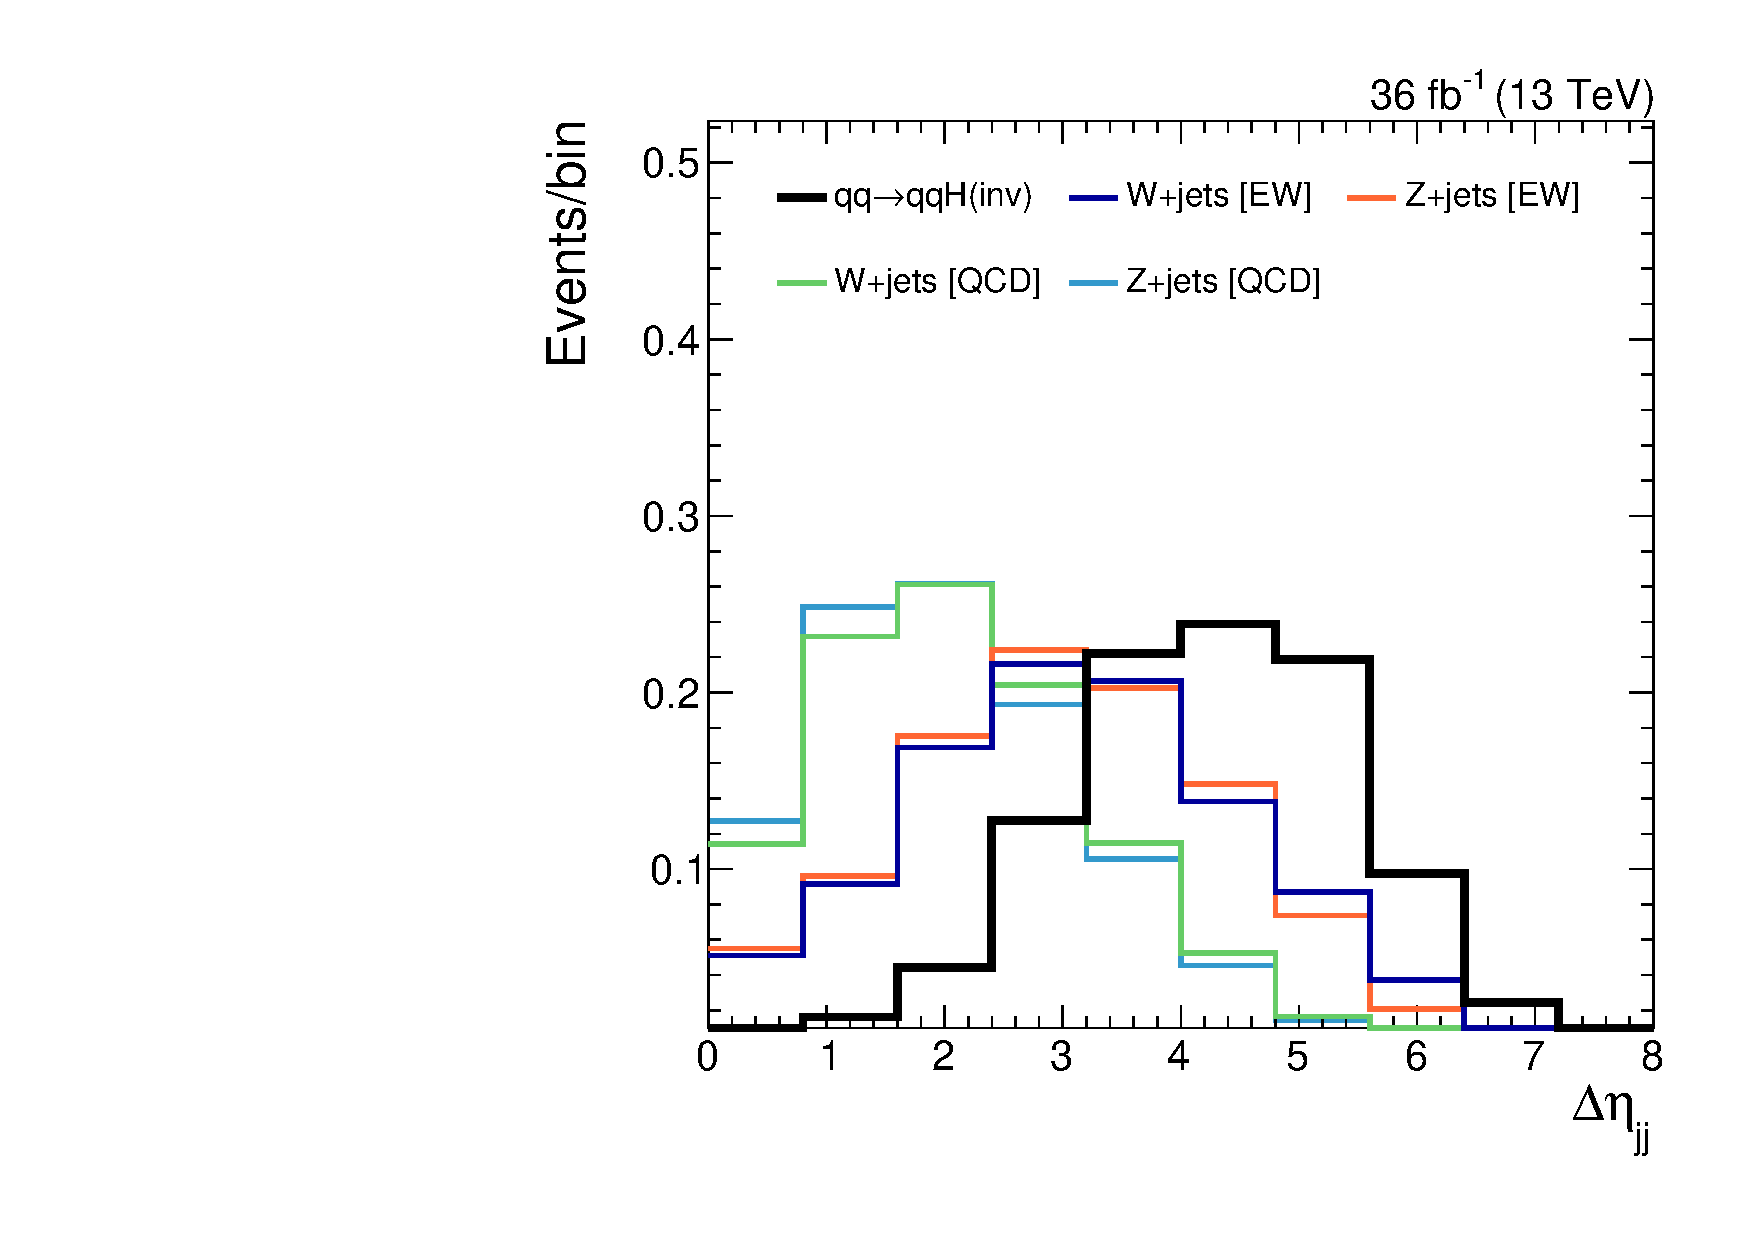
\includegraphics[width=\textwidth]{figures/vbf/shapes/loosesignal_jot12DEta.pdf}
            \caption{\deta}
        \end{subfigure}
        \begin{subfigure}[t]{0.32\textwidth}
            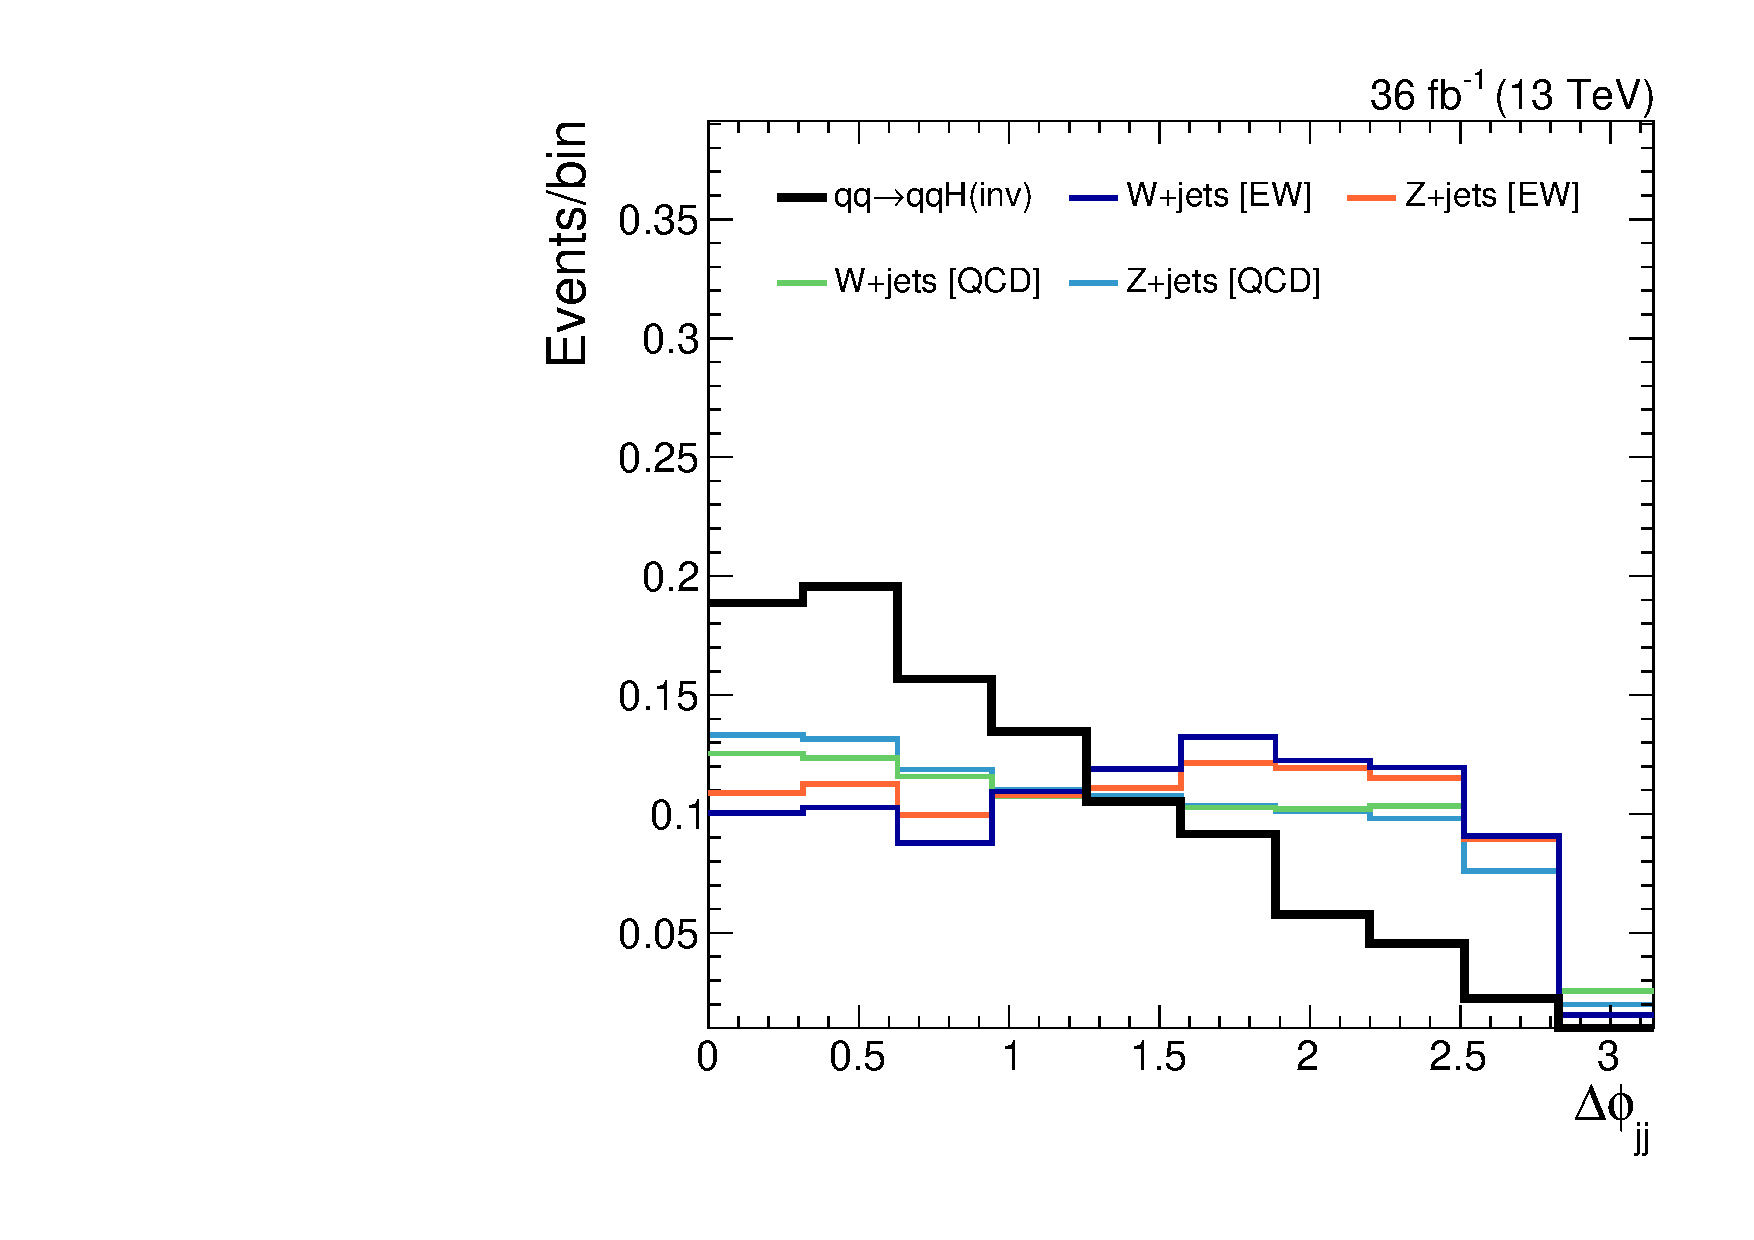
\includegraphics[width=\textwidth]{figures/vbf/shapes/loosesignal_jot12DPhi.pdf}
            \caption{\dphi}
        \end{subfigure}
        \caption{VBF tag observable distributions, as compared between $H$ vs $Z$ vs $W$ production, and VBF vs QCD modes.}
        \label{fig:vbf:dijetkins}
    \end{center}
\end{figure}

\subsection{Sensitivity optimization}

A \emph{baseline} selection is defined as:
\begin{itemize}
    \item $\ptmiss>250$ GeV: driven by trigger efficiency, as discussed in Section~\ref{sec:vbf:trig}.
    \item $\pt^\mathrm{jet}>80,40$ GeV: require two VBF jets, lower $\pt$ thresholds set by trigger efficiency
    \item $N_{e,\mu,\tau,\gamma}=0$: veto leptonic decays of $Z$ and $W$, $t\bar{t}$, diboson production, $\gamma$+jet, etc.
    \item $\min\Delta\phi(\mathrm{jet},\ptmiss)>0.4$: remove QCD multijet events.
    \item $|p^\mathrm{miss}_\mathrm{T,calo}-\ptmiss|<\ptmiss/2$: remove miscalibrated events.
\end{itemize}

As the tag variables each offer some level of separation between signal and backgrounds, we can choose to either fit the distributions or use them to select events. 
To find the optimal choice, we fit each of the distributions in turn, and scan the other two observables.
The details of this fit and the background estimation are described in Section~\ref{sec:vbf:bkg}.
The metric is chosen to be the expected 95\% CLs upper limit on $\mathcal{B}(\hinv)$.
Figure~\ref{fig:vbf:opt} shows the result of this optimization.
With appropriate selection critera, fitting either $m_{jj}$ and $\Delta\eta_{jj}$ gives an optimal expected limit of $0.23$.
Of the two options, we choose to fit $m_{jj}$ and require $\Delta\eta_{jj}>1$ and $\Delta\phi_{jj}<1.5$.

\begin{figure}[]
    \begin{center}
        \begin{subfigure}[t]{0.32\textwidth}
            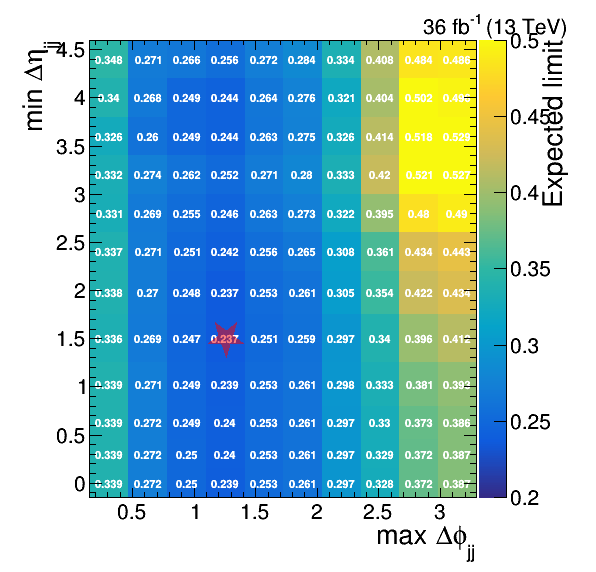
\includegraphics[width=\textwidth]{figures/vbf/opt/optimized_scan_deta_fabsdphi.png}
            \caption{Fit \mjj}
        \end{subfigure}
        \begin{subfigure}[t]{0.32\textwidth}
            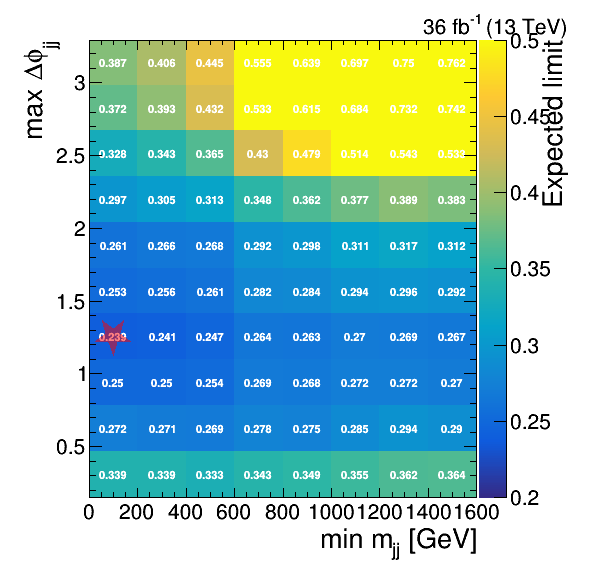
\includegraphics[width=\textwidth]{figures/vbf/opt/optimized_scan_fabsdphi_mjj.png}
            \caption{Fit \deta}
        \end{subfigure}
        \begin{subfigure}[t]{0.32\textwidth}
            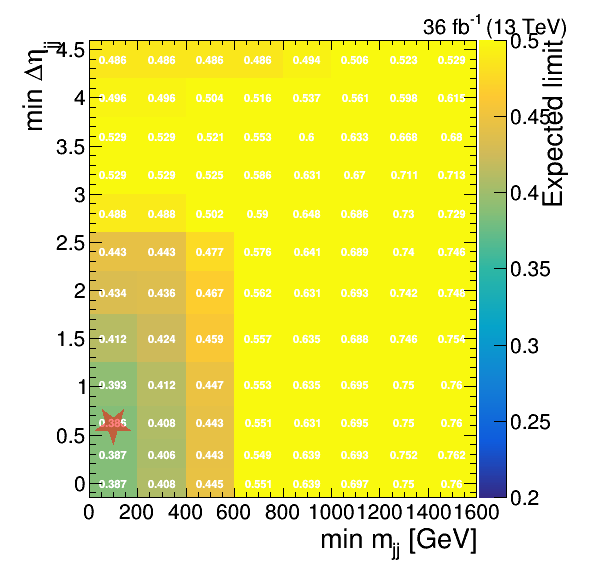
\includegraphics[width=\textwidth]{figures/vbf/opt/optimized_scan_deta_mjj.png}
            \caption{Fit \dphi}
        \end{subfigure}
        \caption{Optimization of the dijet kinematic selection.
                 Each plot corresponds to fitting the labelled distribution, while scanning the other two VBF tag observables as selection criteria.
                 The color $z$-axis is the expected 95\% CLs upper limit on the invisible branching ratio of the Higgs boson.
                 The optimal selection criteria for each fit distribution is indicated with a red star.}
        \label{fig:vbf:opt}
    \end{center}
\end{figure}

\section{Background estimation}
\label{sec:vbf:bkg}

To estimate the combined $m_{jj}$ spectra of the EW and QCD $V$+jet backgrounds, we employ a similar visible-to-invisible strategy as described in Section~\ref{sec:mt:bkg}.
In this case, the transfer factors $\T{}{}$ are a function of $m_{jj}$.
Control regions are defined using dilepton (single-lepton) selections to estimate the $Z$ ($W$) contributions.
Again, $\ptmiss$ is replaced by $U$ (Equation~\ref{eq:mt:u}) to mimic the signal region selection. 
Because there are \emph{two} components to estimate in each CR (QCD and EW), we slightly modify the likelihood.
Adding only the $\mu\mu$ CR to constrain the $Z$+jet component for now:
\begin{align}
    \mathcal{L}(\bm{d} \,|\, \mu,\muz,\bm{\theta}) = & \prod_{i\in\mathrm{bins}} \left[
    \pois\left(d^{\mathrm{SR}}_{i} ~\Big|~ \mu S^{\mathrm{SR}}_{i}(\bm\theta)  + \muzi + \frac{\muzi}{\Ti{\mathrm{QE}}{Z}(\bm\theta)} + B^{\mathrm{SR}}_{i}(\bm\theta)\right) \right. \nonumber \\
    & \left. \phantom{\prod_{i\in\mathrm{bins}}\Big[} \times \pois\left(d^{\mu\mu}_i~\Big|~ \frac{\muzi}{\Ti{\mu\mu}{Z}(\bm\theta)} + \frac{\muzi}{\Ti{\mu\mu}{Z}(\bm\theta) \Ti{\mathrm{QE}}{Z}(\bm\theta)} + B^{\mu\mu}_i(\bm\theta) \right)\right]  \nonumber \\ 
    & \times  \prod_{j=0}^{n_\theta} p_j(\theta_j)
\end{align}
While the notation largely follows that used in Equation~\ref{eq:mt:lhood}, one additional term has been introduced.
This is a \emph{transfer factor} linking the QCD and EW components in the signal region, so that the only free parameter is $\muz$:
\begin{equation}
    \Ti{\mathrm{QE}}{Z} = \frac{N^\mathrm{SR}_i(\mathrm{QCD\,}Z\rightarrow\nu\nu)}{N^\mathrm{SR}_i(\mathrm{EW\,}Z\rightarrow\nu\nu)} 
\end{equation}
where as always, the yields $N$ are predicted using MC. 
Kinematic distributions from the two dilepton CRs are shown in Figure~\ref{fig:vbf:zcr}.

\begin{figure}[]
    \begin{center}
        \begin{subfigure}[t]{0.24\textwidth}
            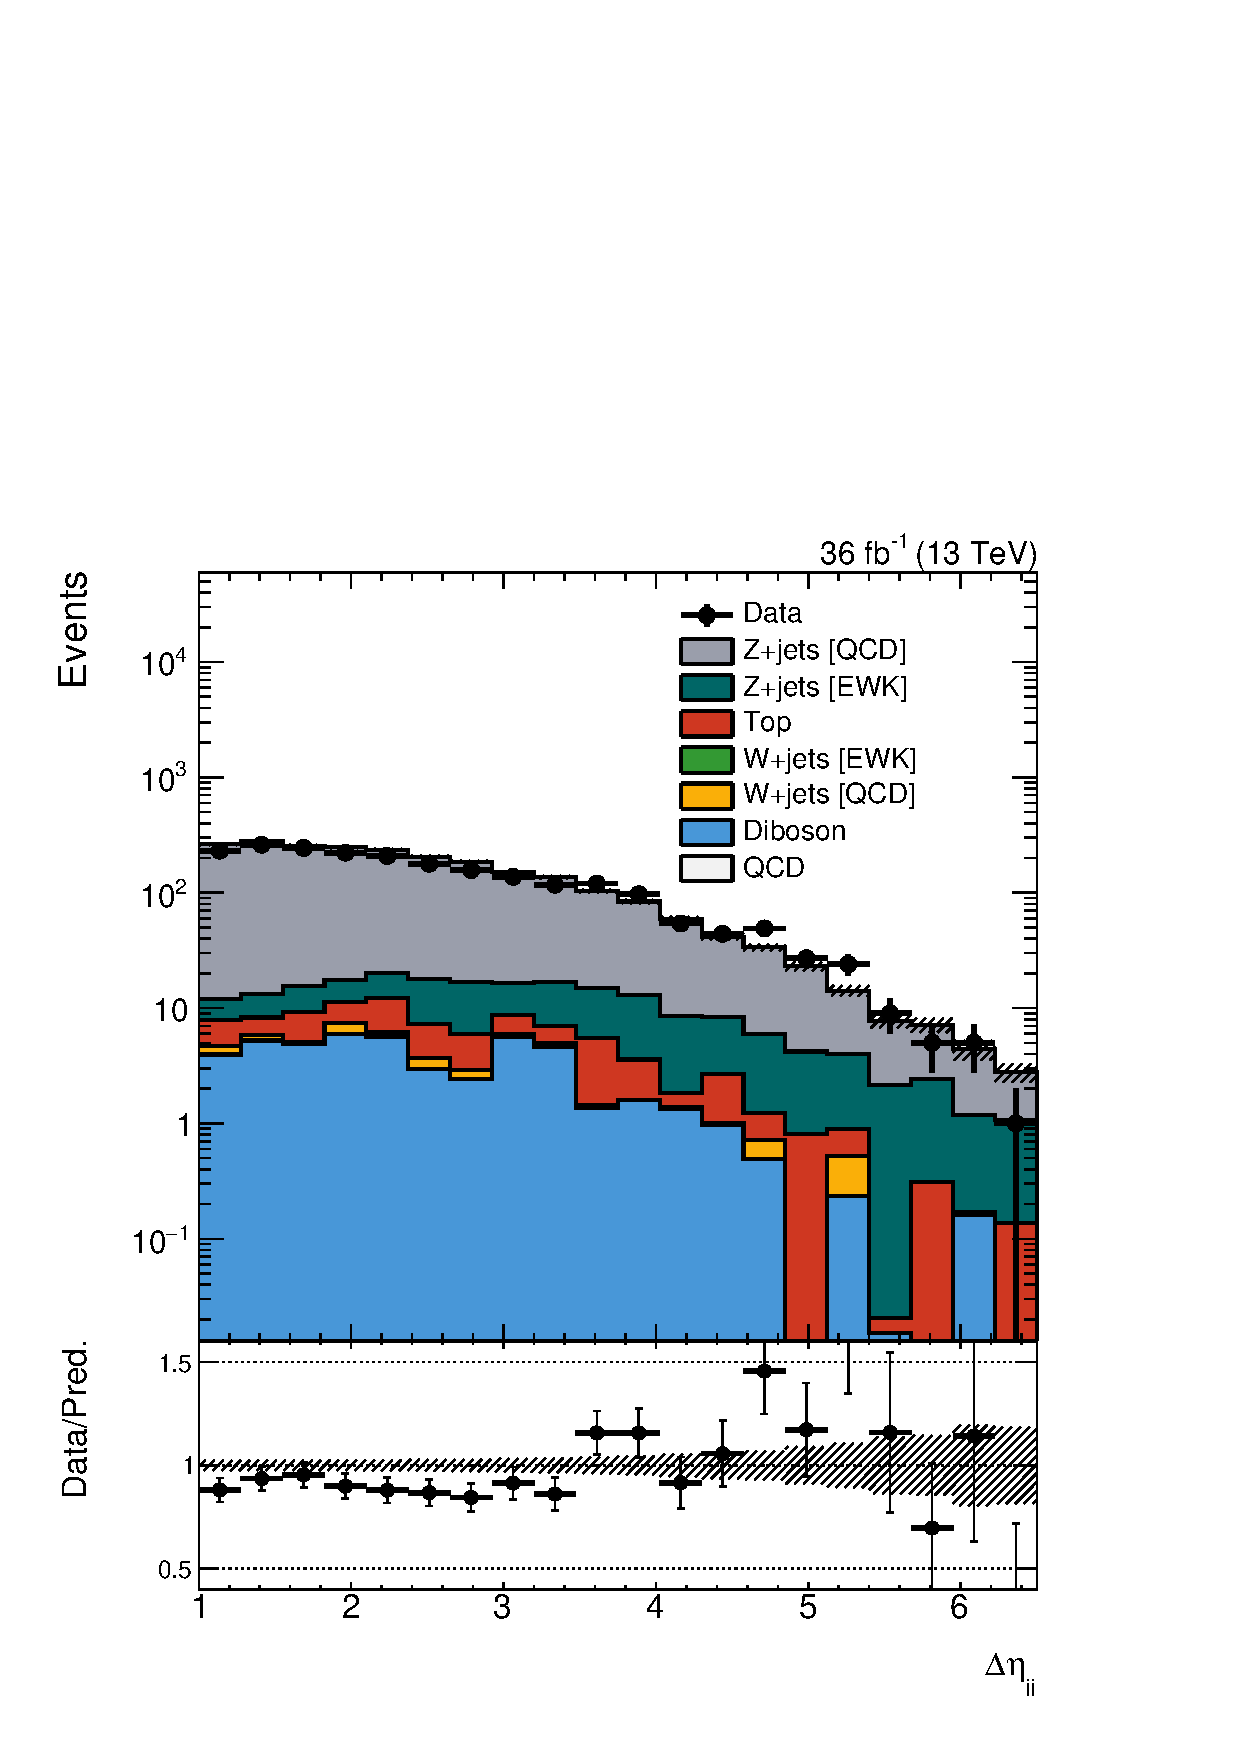
\includegraphics[width=\textwidth]{figures/vbf/prefit/dielectron_jot12DEta_logy.pdf}
        \end{subfigure}
        \begin{subfigure}[t]{0.24\textwidth}
            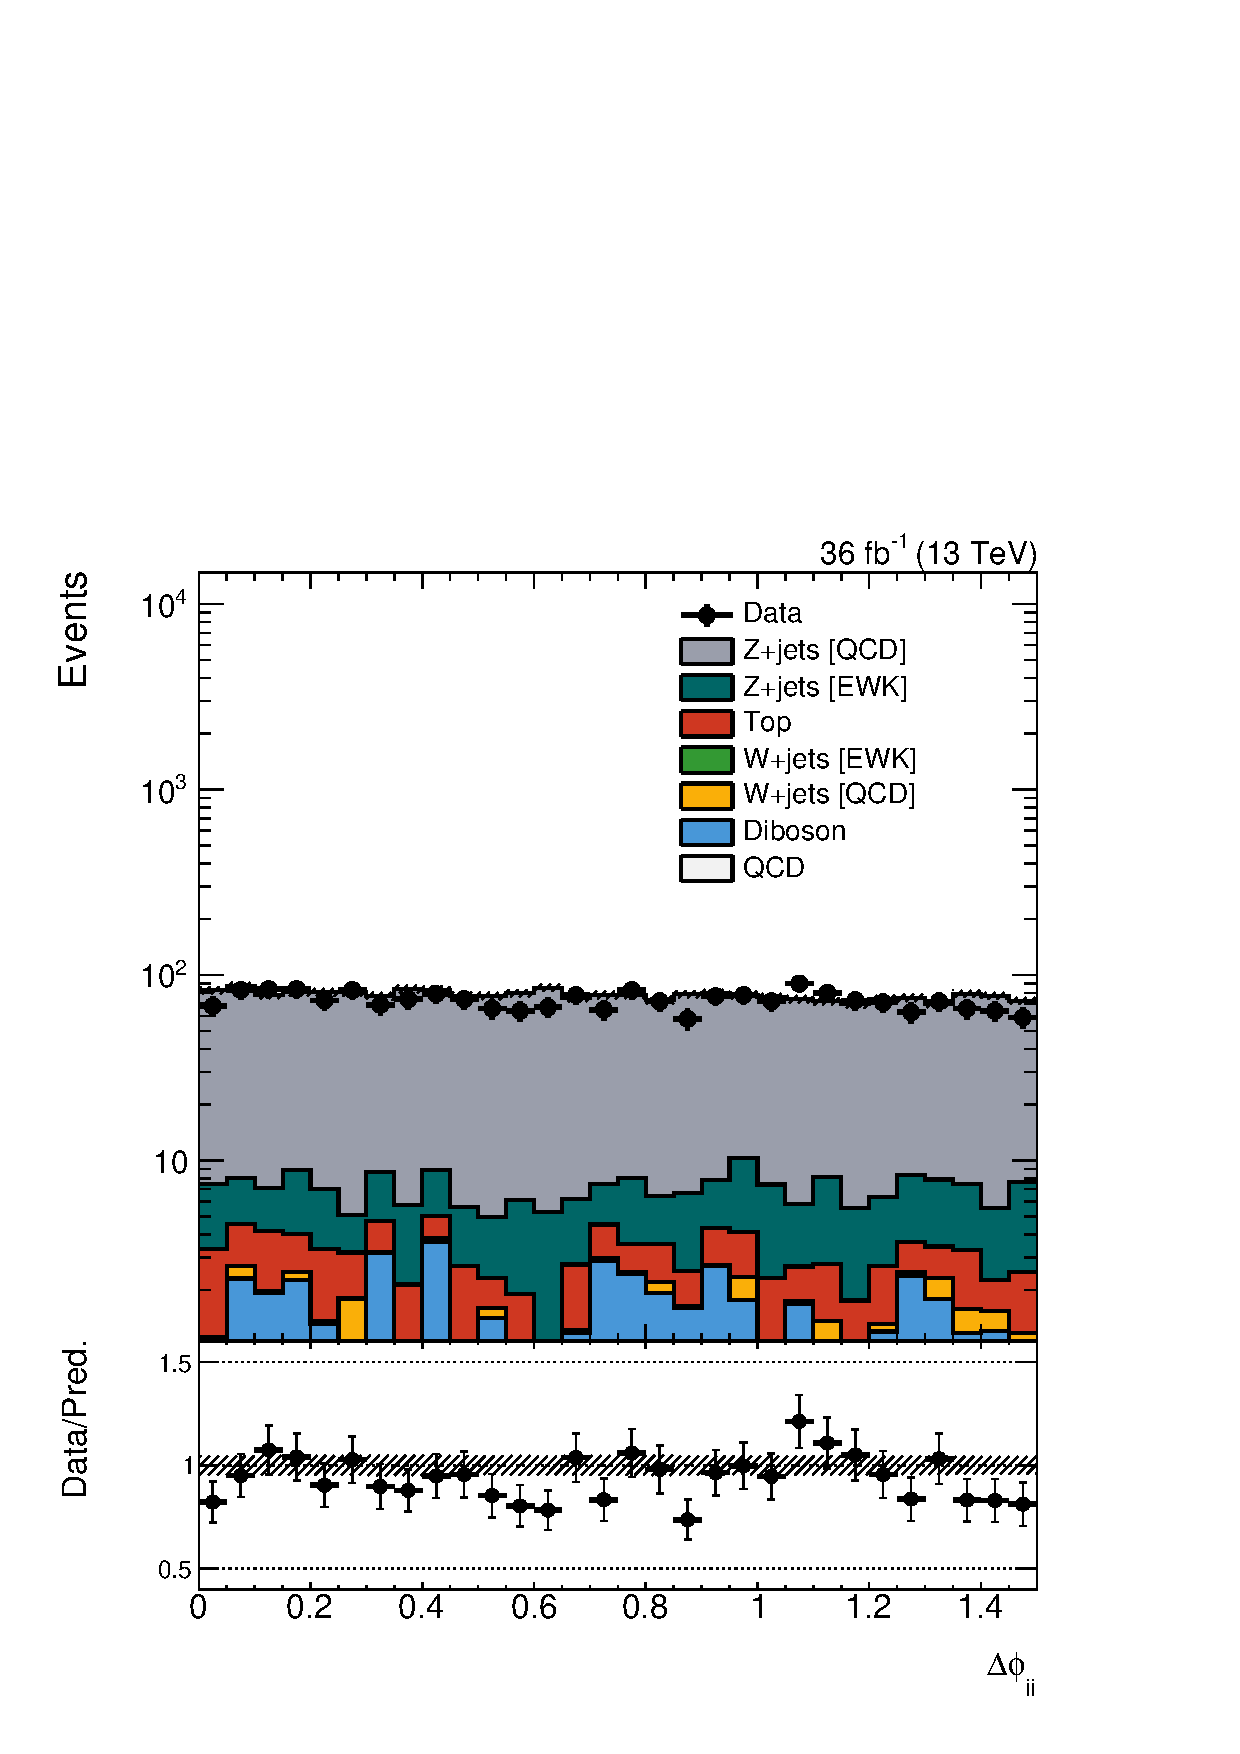
\includegraphics[width=\textwidth]{figures/vbf/prefit/dielectron_jot12DPhi_logy.pdf}
        \end{subfigure}
        \begin{subfigure}[t]{0.24\textwidth}
            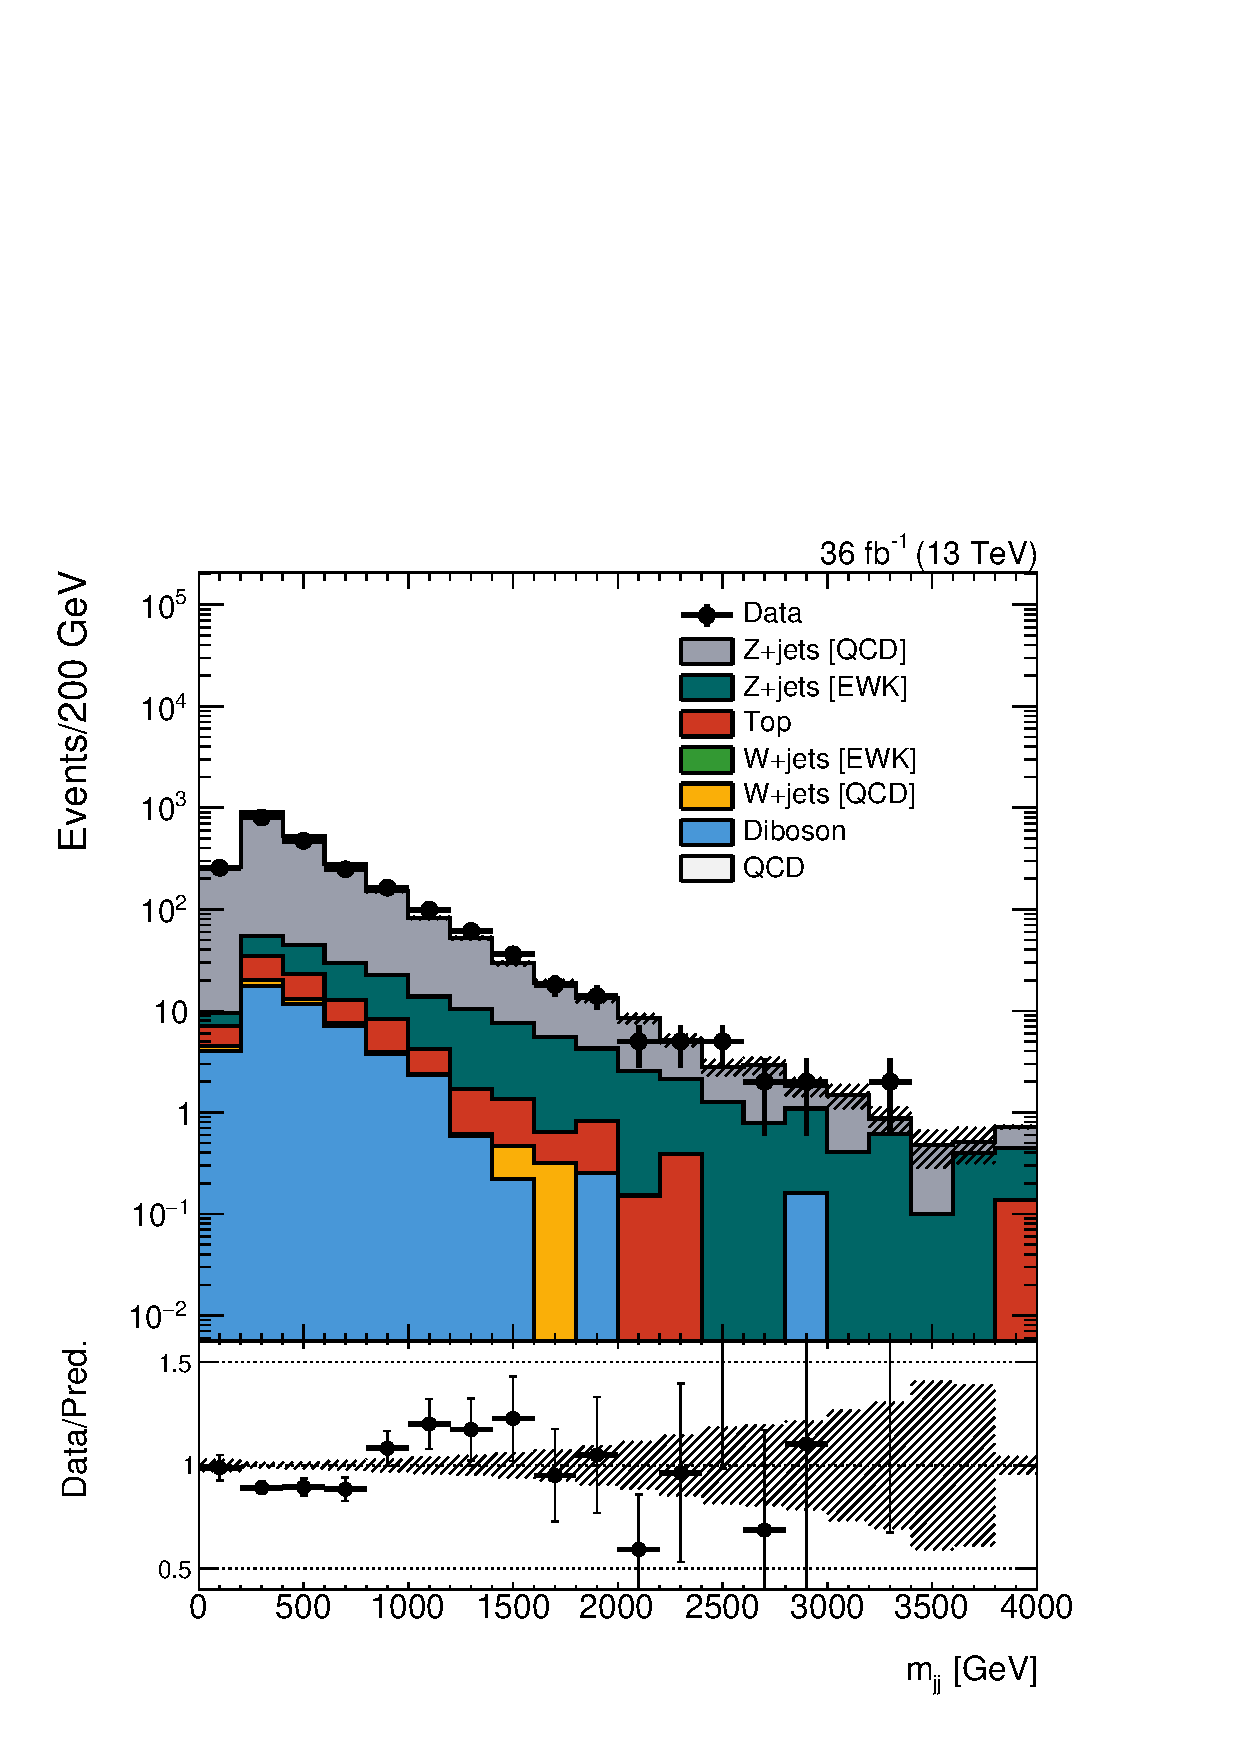
\includegraphics[width=\textwidth]{figures/vbf/prefit/dielectron_jot12Mass_logy.pdf}
        \end{subfigure}
        \begin{subfigure}[t]{0.24\textwidth}
            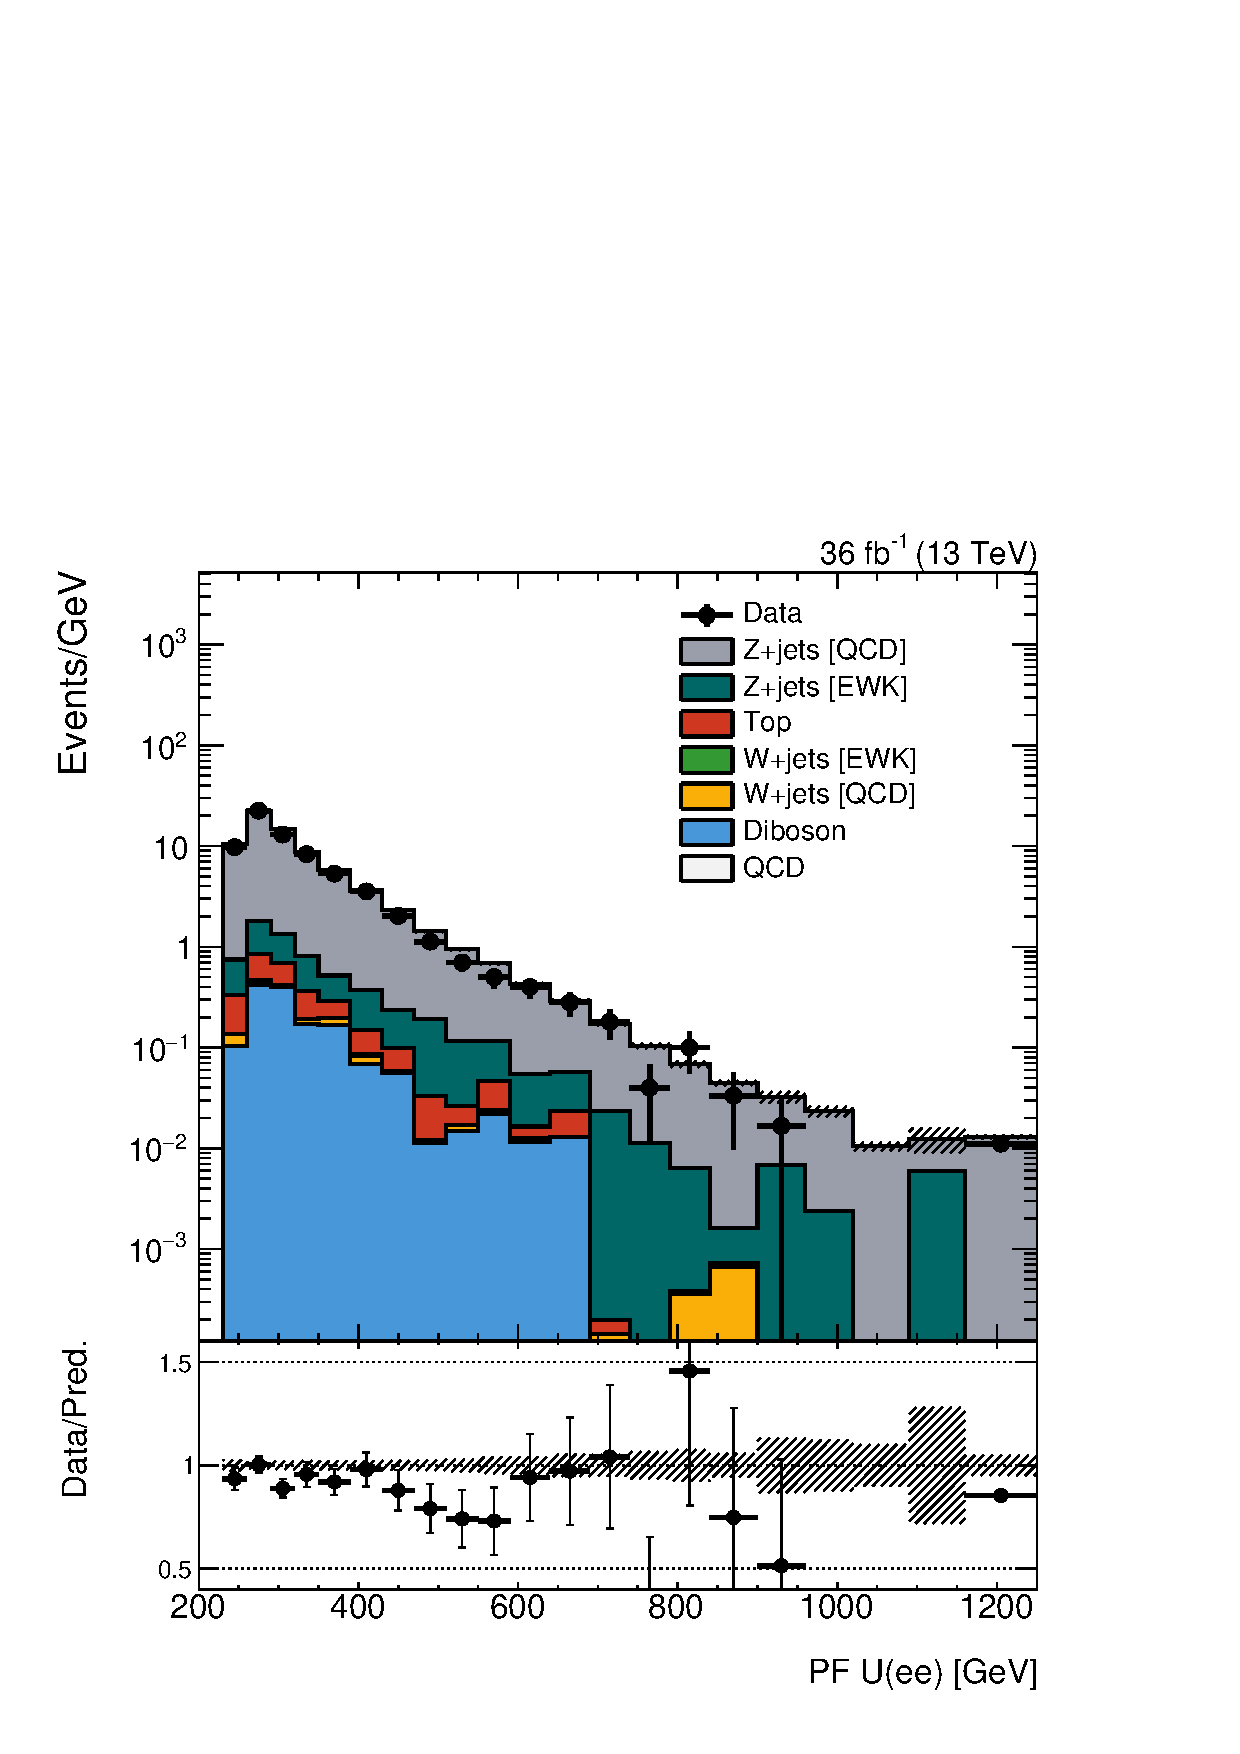
\includegraphics[width=\textwidth]{figures/vbf/prefit/dielectron_pfUZmag_logy.pdf}
        \end{subfigure} \\ 
        \begin{subfigure}[t]{0.24\textwidth}
            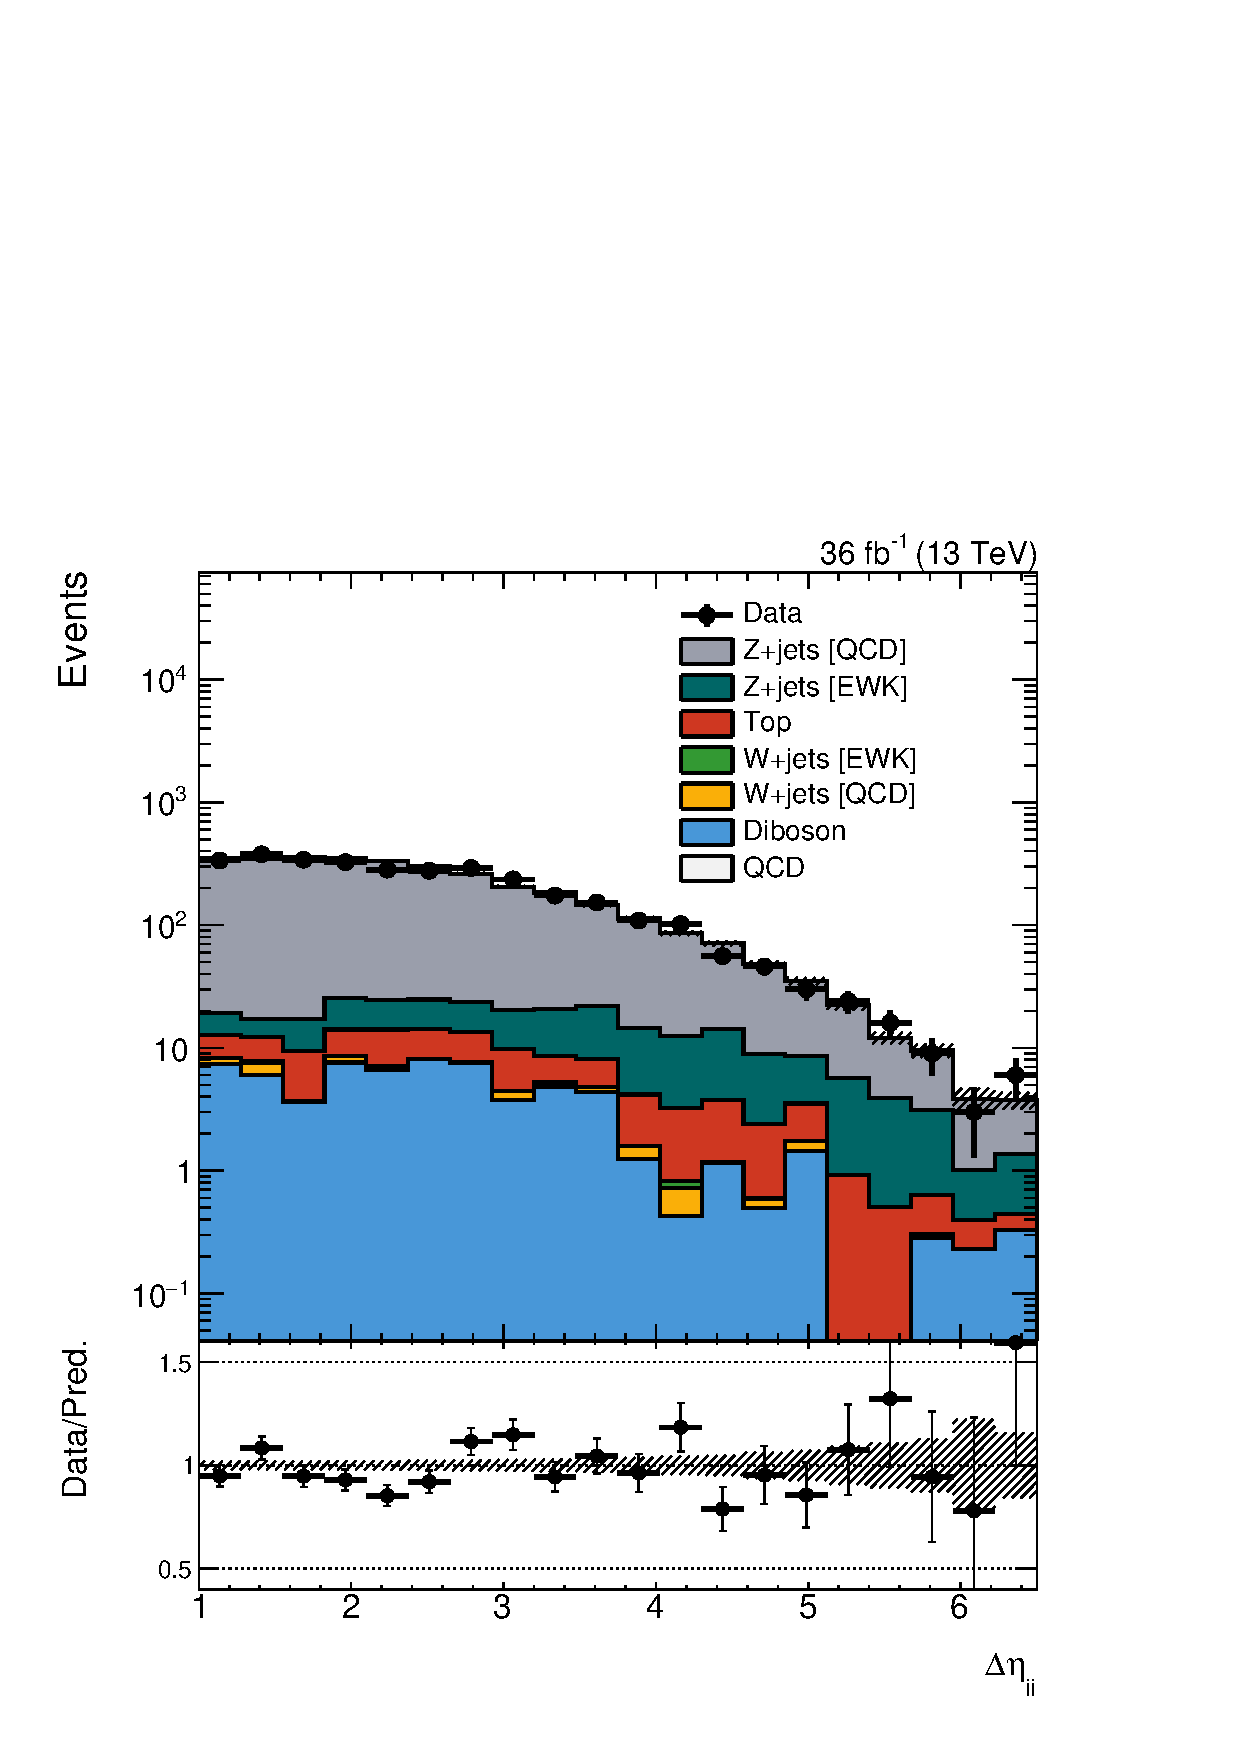
\includegraphics[width=\textwidth]{figures/vbf/prefit/dimuon_jot12DEta_logy.pdf}
        \end{subfigure}
        \begin{subfigure}[t]{0.24\textwidth}
            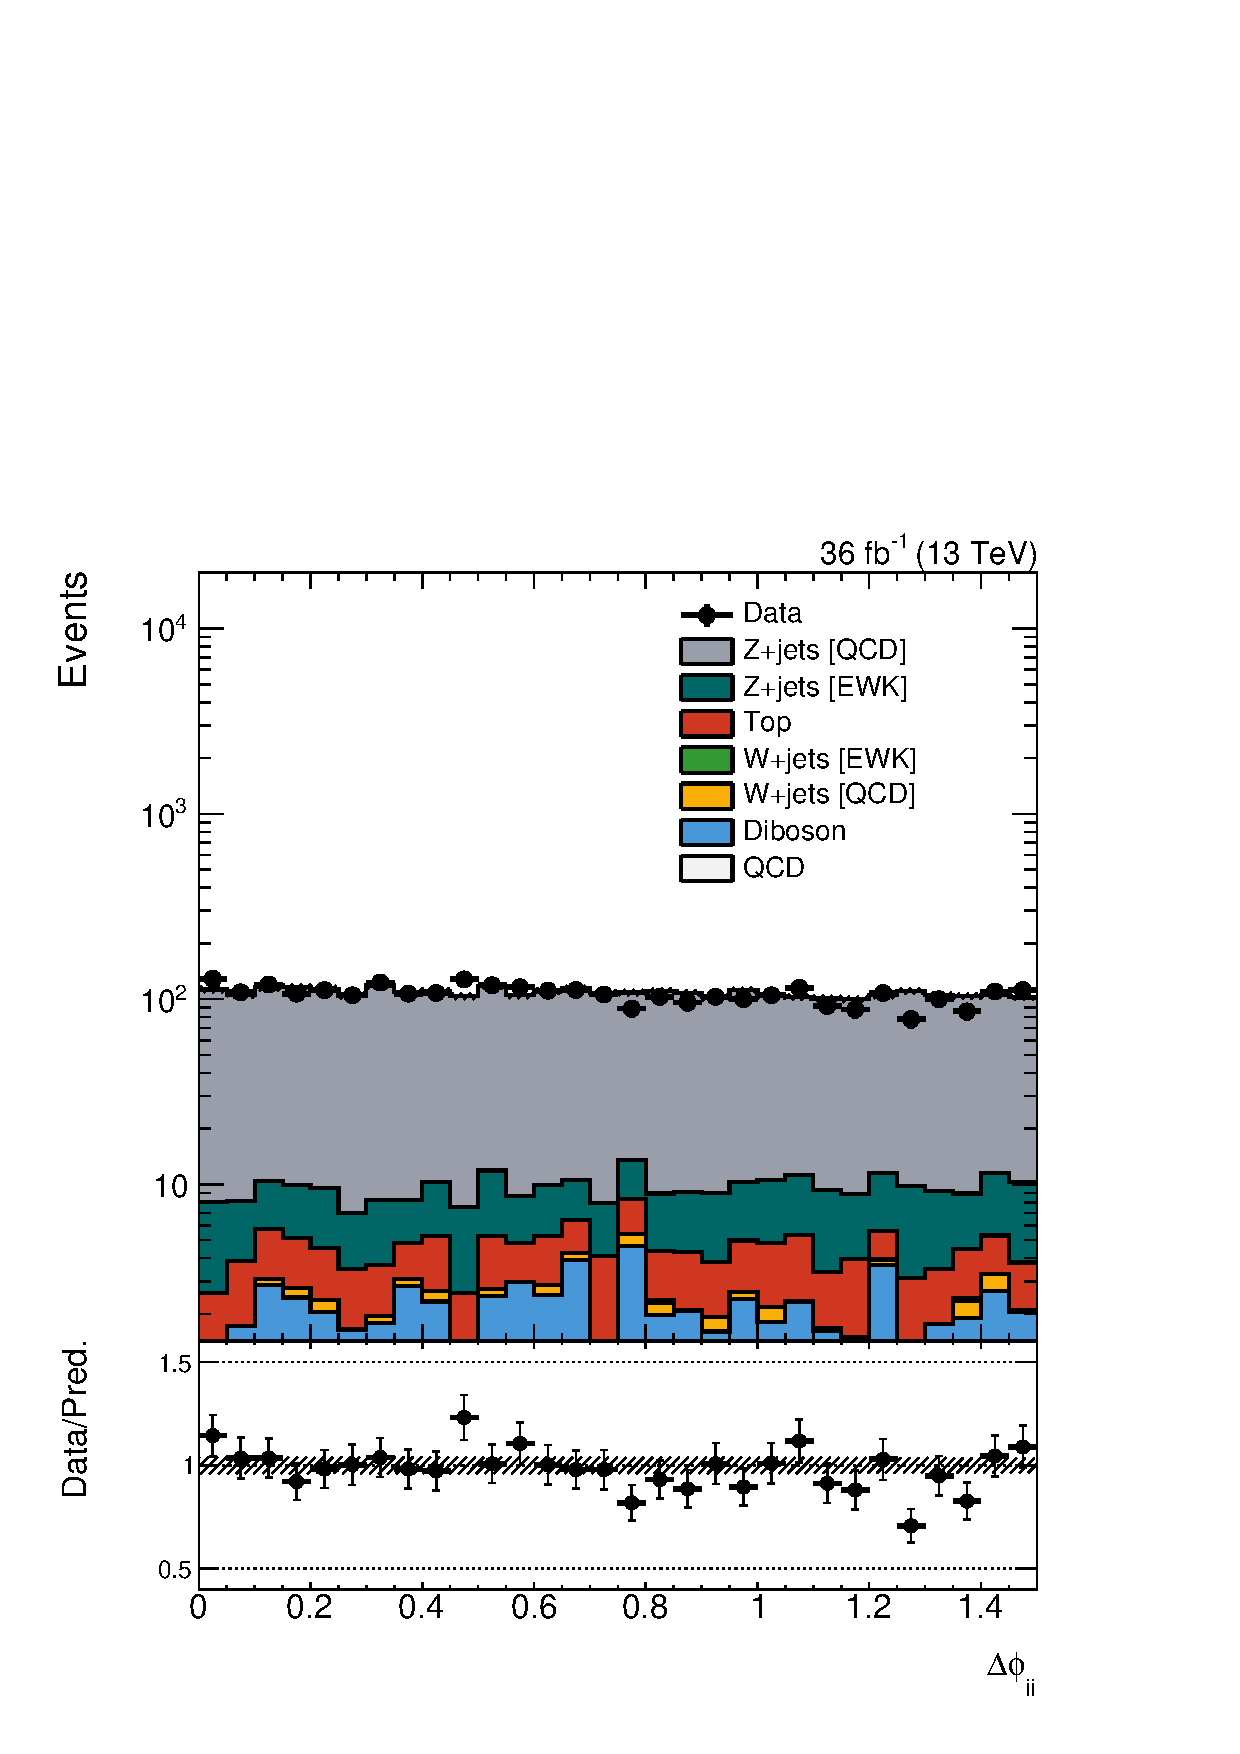
\includegraphics[width=\textwidth]{figures/vbf/prefit/dimuon_jot12DPhi_logy.pdf}
        \end{subfigure}
        \begin{subfigure}[t]{0.24\textwidth}
            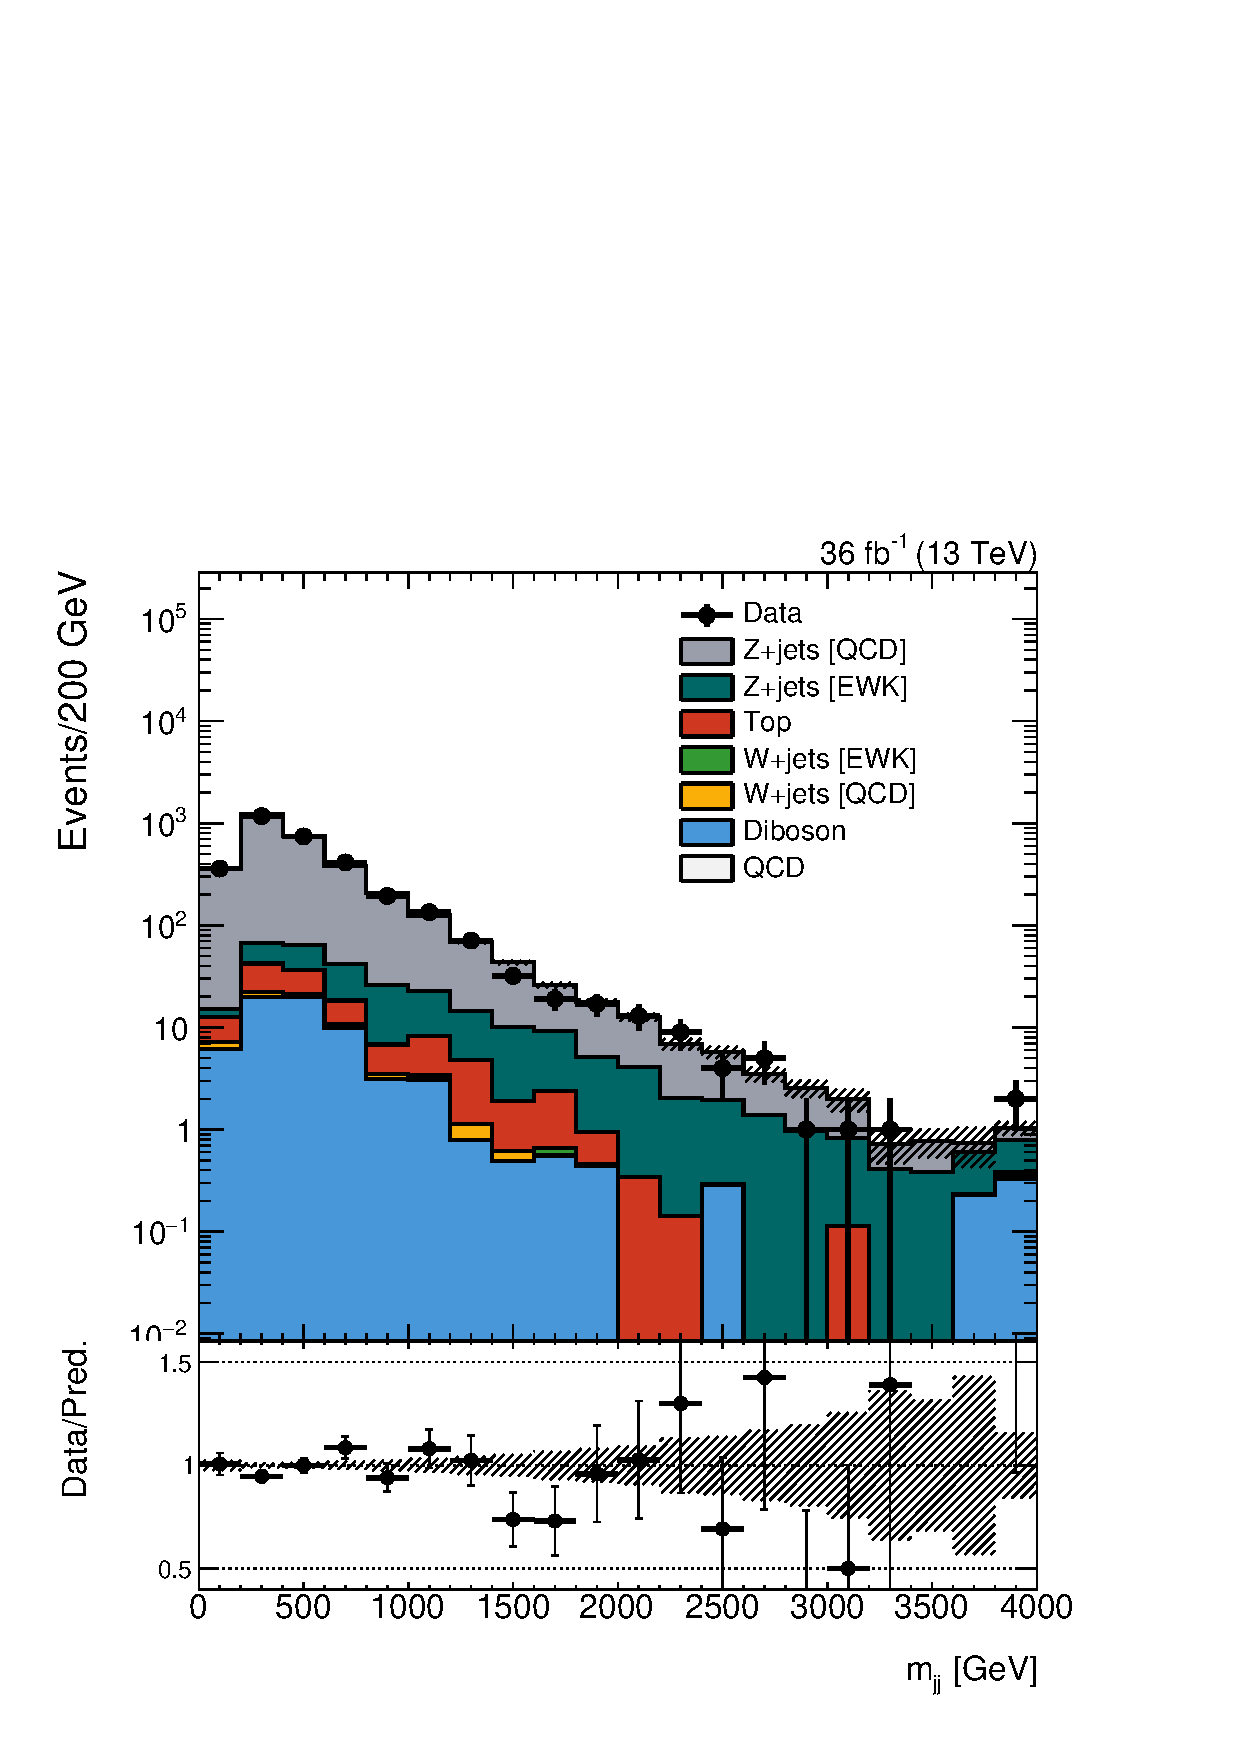
\includegraphics[width=\textwidth]{figures/vbf/prefit/dimuon_jot12Mass_logy.pdf}
        \end{subfigure}
        \begin{subfigure}[t]{0.24\textwidth}
            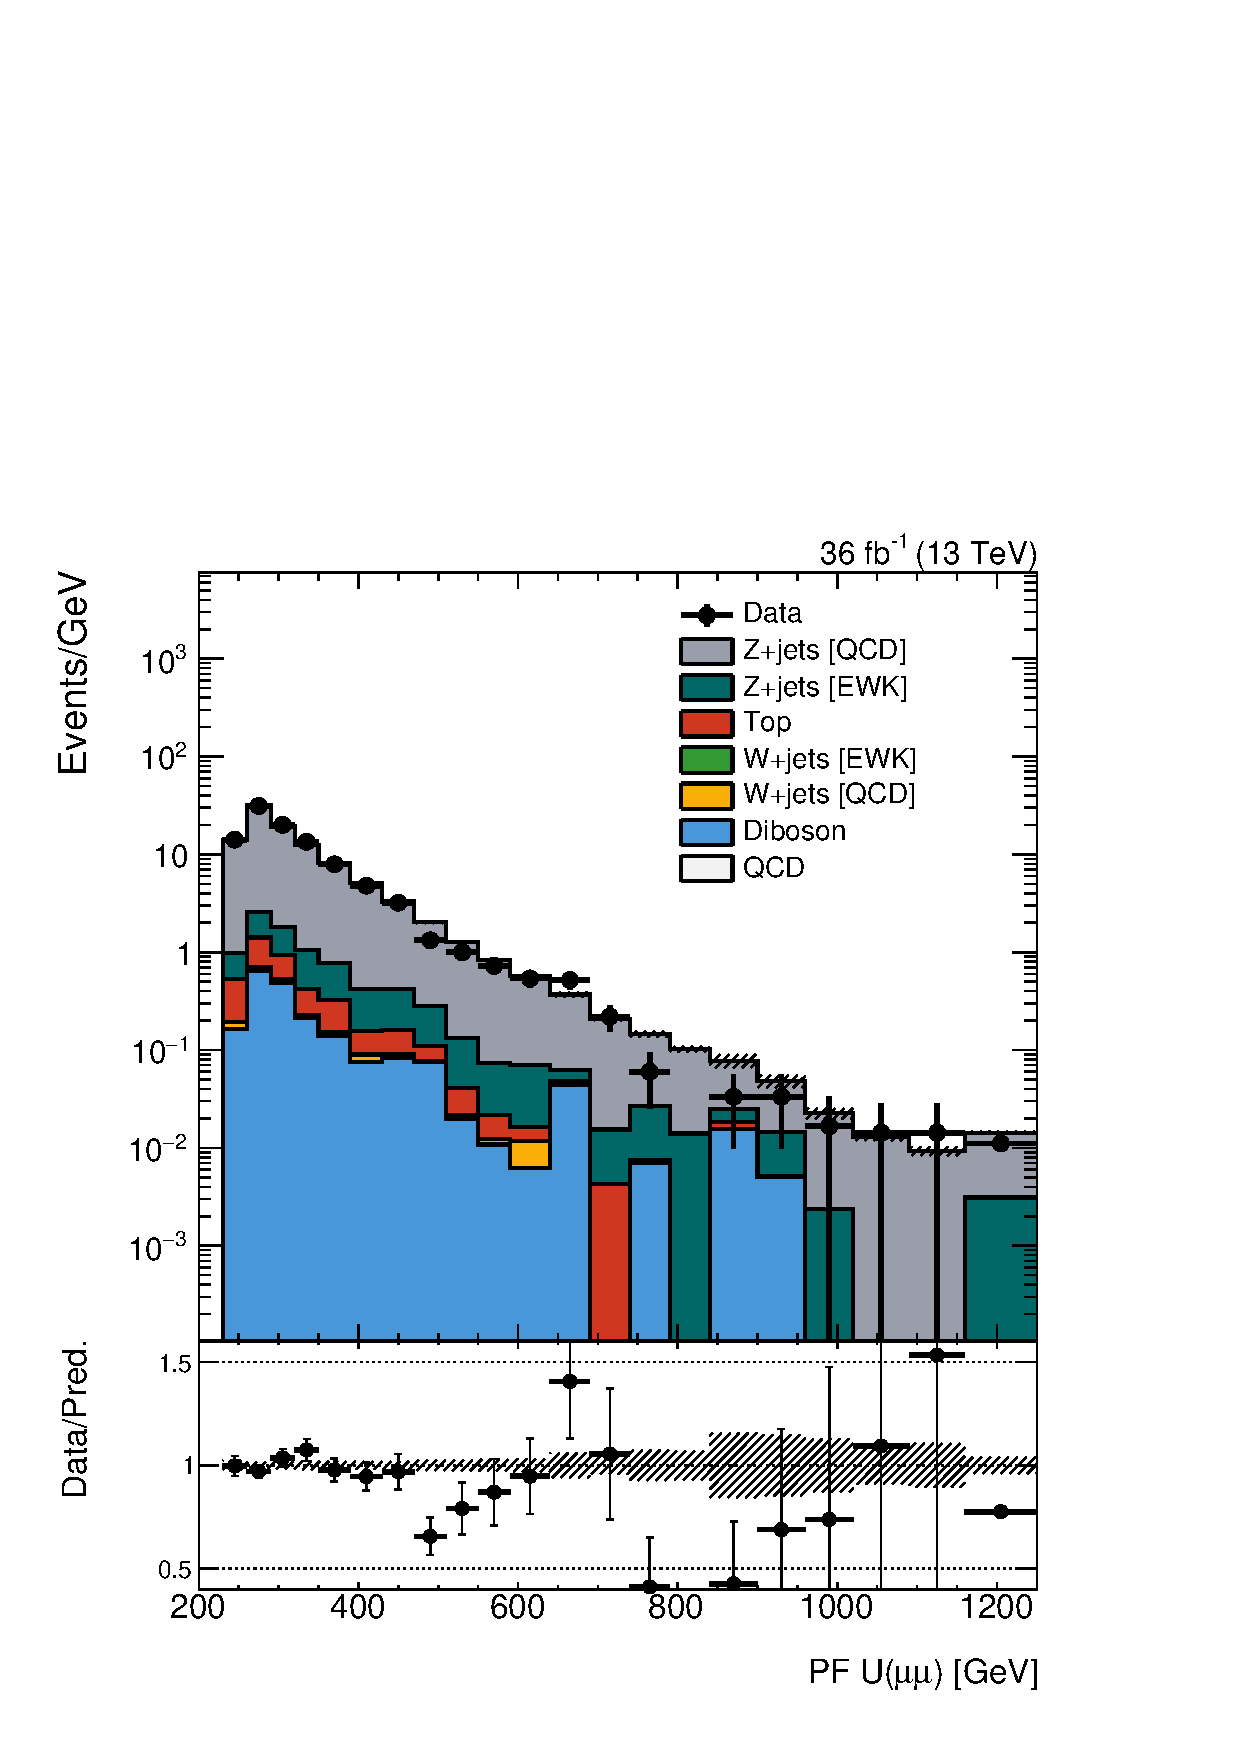
\includegraphics[width=\textwidth]{figures/vbf/prefit/dimuon_pfUZmag_logy.pdf}
        \end{subfigure}
        \caption{Dijet and recoil distributions in the dielectron (top) and dimuon (bottom) CRs.
                 All predicted distributions are prior to the maximization of the likelihood, and the grey band refers only to the statistical uncertainty of the MC.
                 The pre-fit MC describes the observed data reasonably well.
        }
        \label{fig:vbf:zcr}
    \end{center}
\end{figure}

In the region $m_{jj}>2.5$ TeV, the statistical power of the dilepton regions is limited.
For this reason, and to estimate the $W$+jets contribution in the SR, we add two single-lepton CRs in analogy to what is done in Section~\ref{sec:mt:bkg}. 
Figure~\ref{fig:vbf:wcr} shows the level of agreement between the data and MC in these CRs.
The likelihood is modified to include the constraints of the single-lepton CRs:
\begin{align}
    \mathcal{L}\left(\bm{d}\,|\, \mu,\muz,\bm{\theta}\right) = \hspace{-30mm} & \nonumber \\
    \prod_{i\in\mathrm{bins}} & \left[
    \pois\left\{d^{\mathrm{SR}}_{i} ~\Big|~ \mu S^{\mathrm{SR}}_{i}(\bm\theta)  + \left(1+\frac{1}{\Ti{\mathrm{QE}}{Z}(\bm\theta)}\right)\left(1+\frac{1}{\Ti{\mathrm{SR}}{Z/W}(\bm\theta)}\right)\muzi + B^{\mathrm{SR}}_{i}(\bm\theta)\right\} \vphantom{\frac{\muzi}{\Ti{\mu\mu}{Z}(\bm\theta)}}\right. \nonumber \\
    & \phantom{\Big[} \times \prod_{X=\mu,e} \pois\left\{d^{X}_i~\Big|~ \left(1+\frac{1}{\Ti{\mathrm{QE}}{Z}(\bm\theta)}\right)\frac{\muzi}{\Ti{X}{W}(\bm\theta)\Ti{\mathrm{SR}}{Z/W}(\bm\theta)} + B^{X}_i(\bm\theta) \right\} \nonumber \\
    & \phantom{\Big[} \times \left.\prod_{X=\mu\mu,ee} \pois\left\{d^{X}_i~\Big|~ \left(1+\frac{1}{\Ti{\mathrm{QE}}{Z}(\bm\theta)}\right)\frac{\muzi}{\Ti{X}{Z}(\bm\theta)} + B^{X}_i(\bm\theta) \right\} \right]  \times  \prod_{j=0}^{n_\theta} p_j(\theta_j)
\end{align}
To validate that the transfer factors are reasonably well-simulated (within the assigned uncertainties), Figure~\ref{fig:vbf:valid} uses the following ratios of CRs as proxies for transfer factors:
\begin{gather}
    \T{\mu\mu}{Z}, \T{ee}{Z} \sim \frac{N_{\mu\mu}(Z\rightarrow\mu\mu)}{N_{ee}(Z\rightarrow ee)} \nonumber \\ 
    \T{\mu}{W}, \T{e}{W} \sim \frac{N_\mu(W\rightarrow\mu\nu)}{N_e(W\rightarrow e\nu)} \nonumber \\ 
    \T{\mathrm{SR}}{Z/W} \sim \frac{N_\mu(W\rightarrow\mu\nu)+N_e(W\rightarrow e\nu)}{N_{\mu\mu}(Z\rightarrow\mu\mu)+N_{ee}(Z\rightarrow ee)} 
\end{gather}

\begin{figure}[]
    \begin{center}
        \begin{subfigure}[t]{0.24\textwidth}
            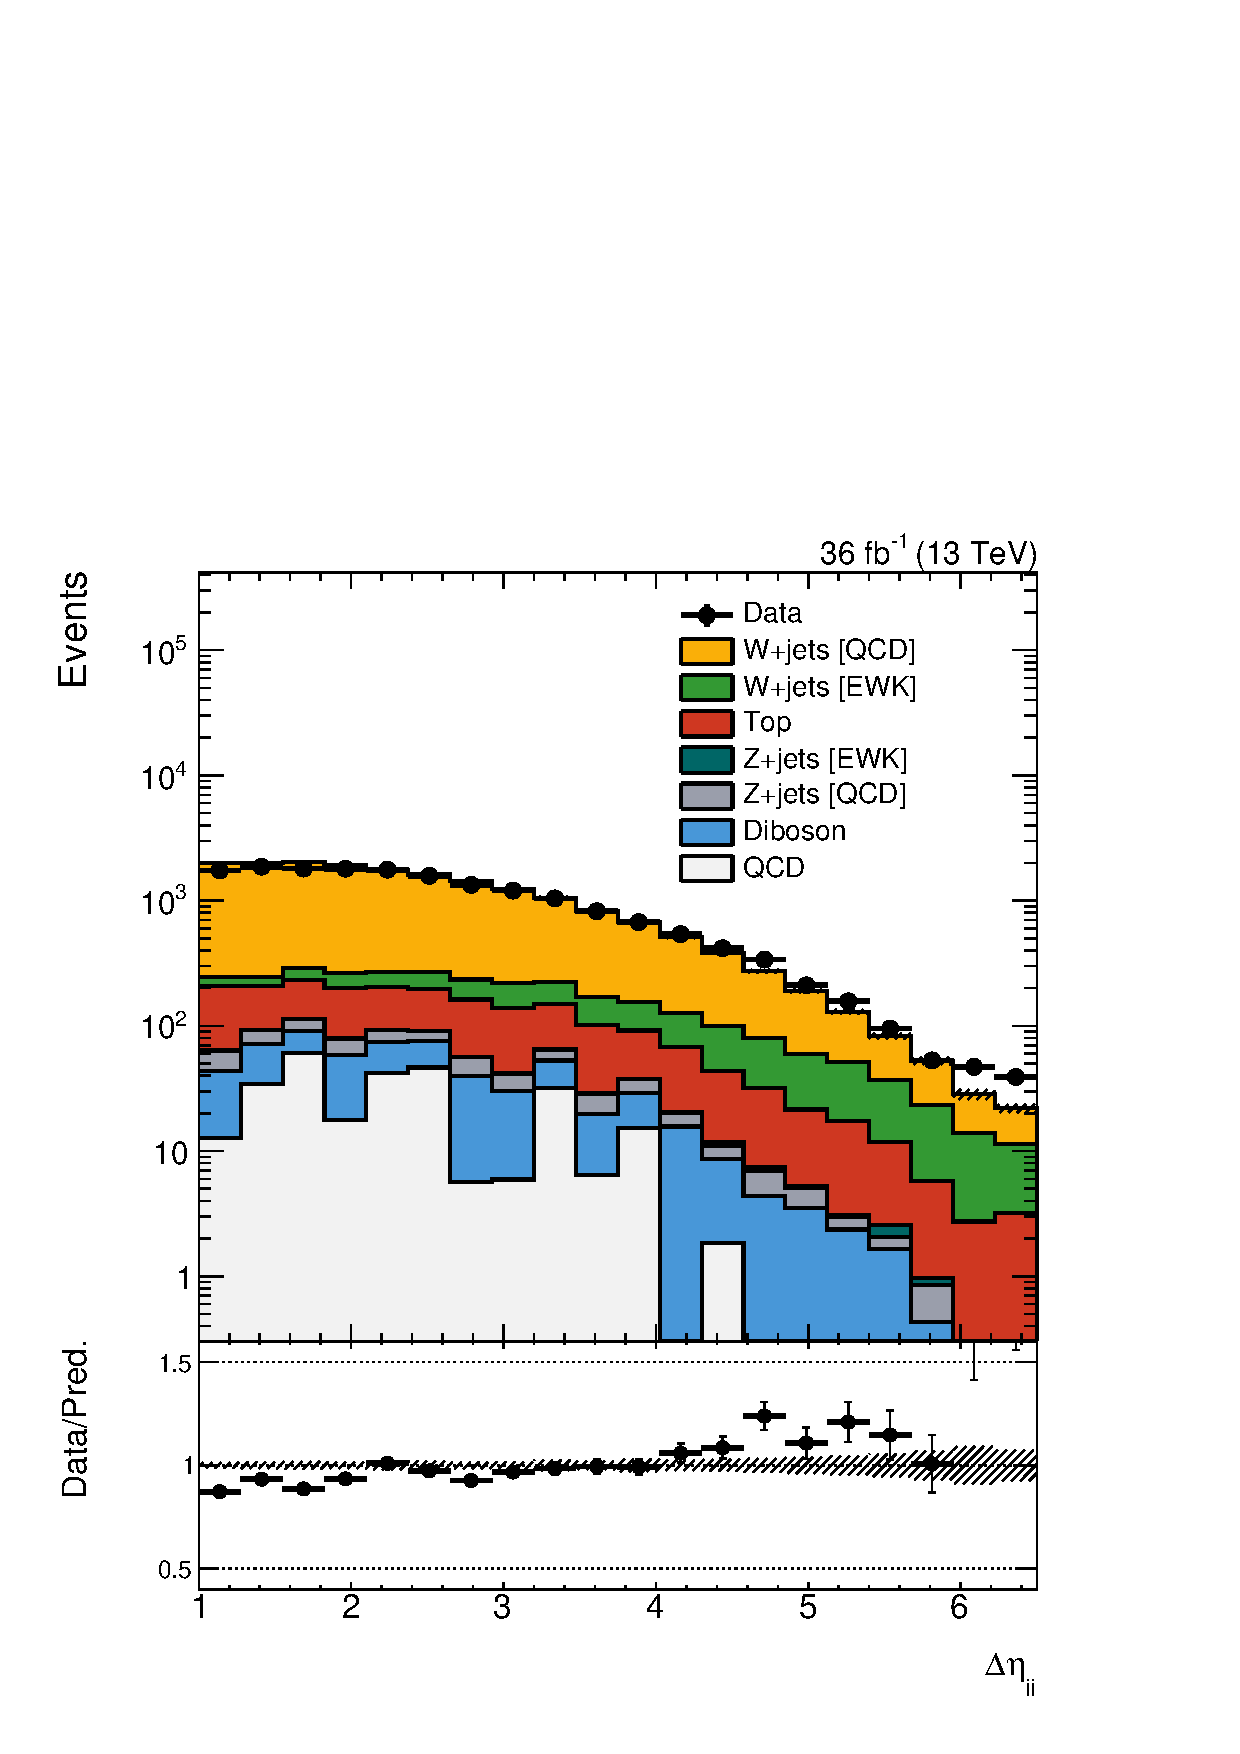
\includegraphics[width=\textwidth]{figures/vbf/prefit/singleelectron_jot12DEta_logy.pdf}
        \end{subfigure}
        \begin{subfigure}[t]{0.24\textwidth}
            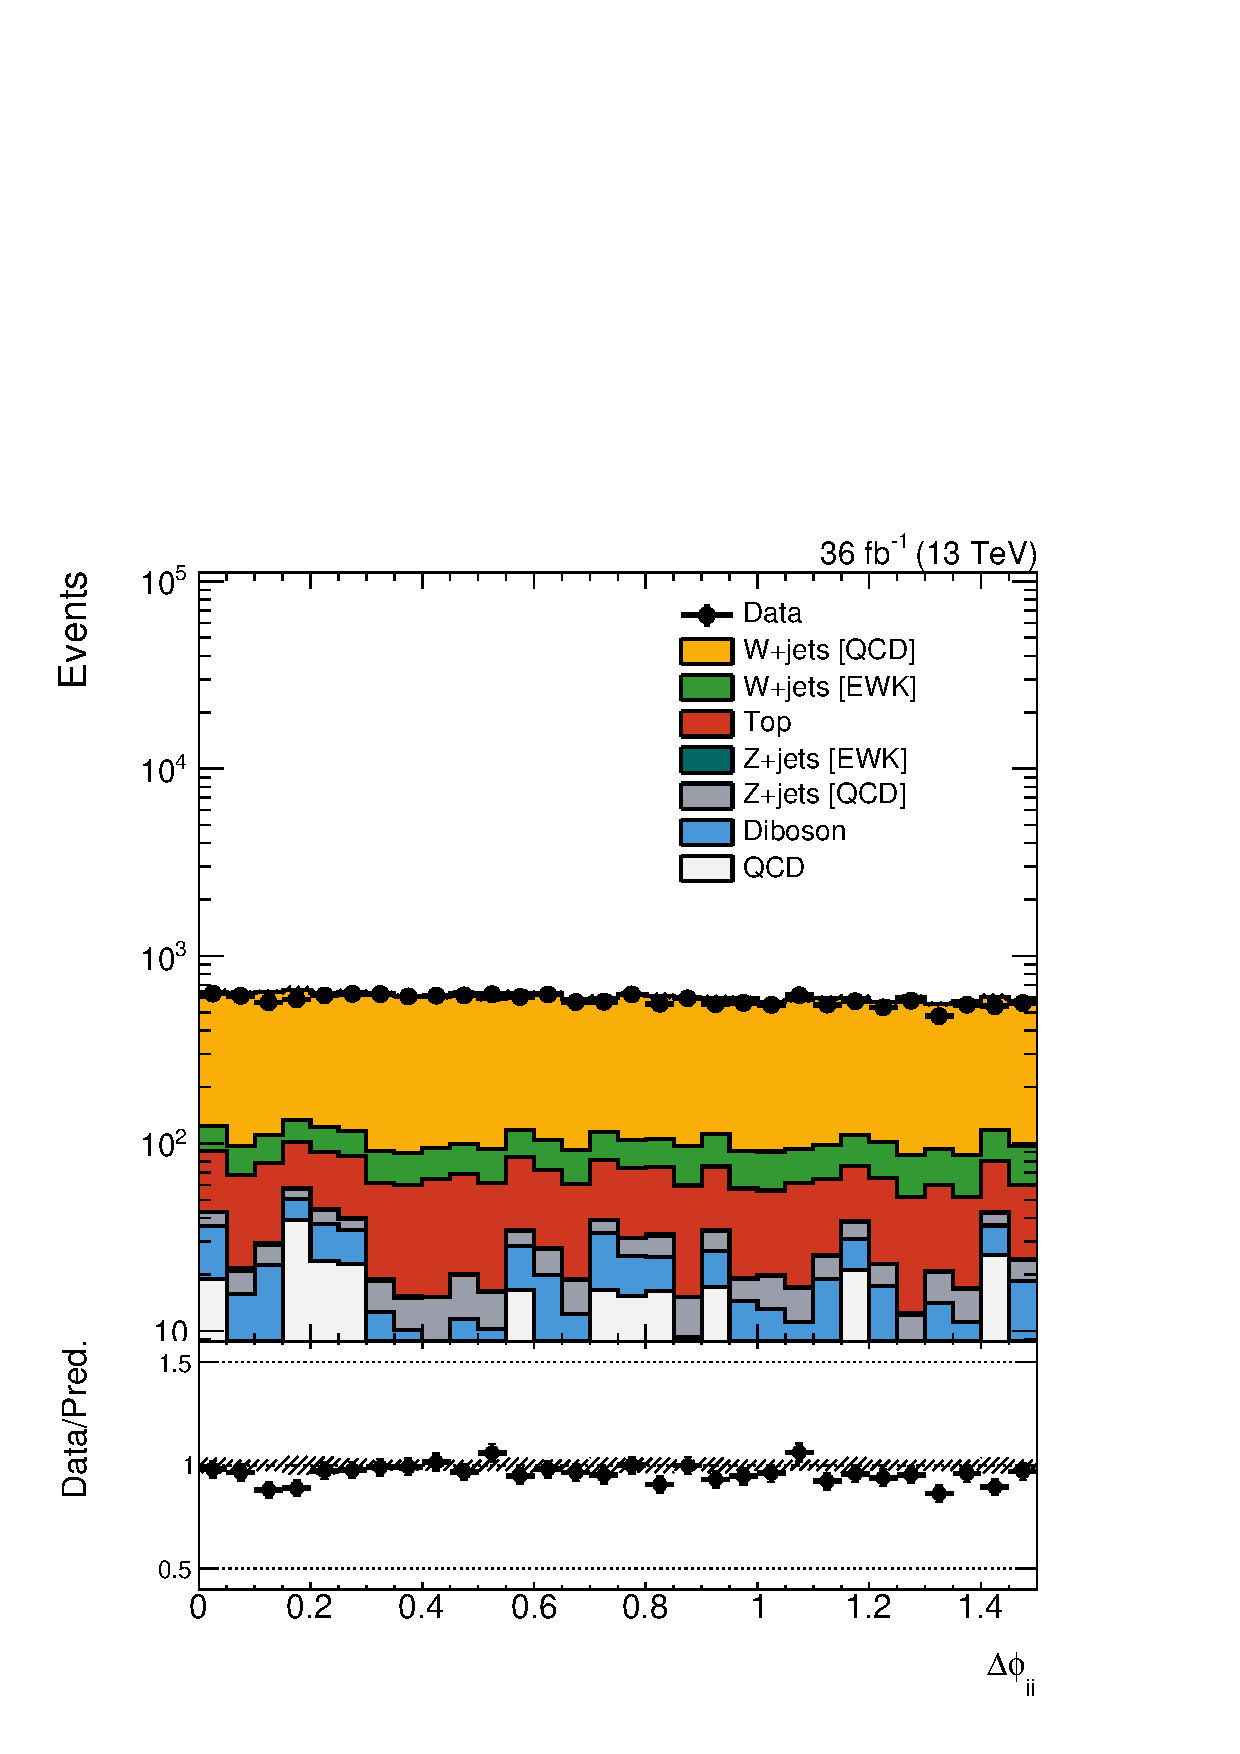
\includegraphics[width=\textwidth]{figures/vbf/prefit/singleelectron_jot12DPhi_logy.pdf}
        \end{subfigure}
        \begin{subfigure}[t]{0.24\textwidth}
            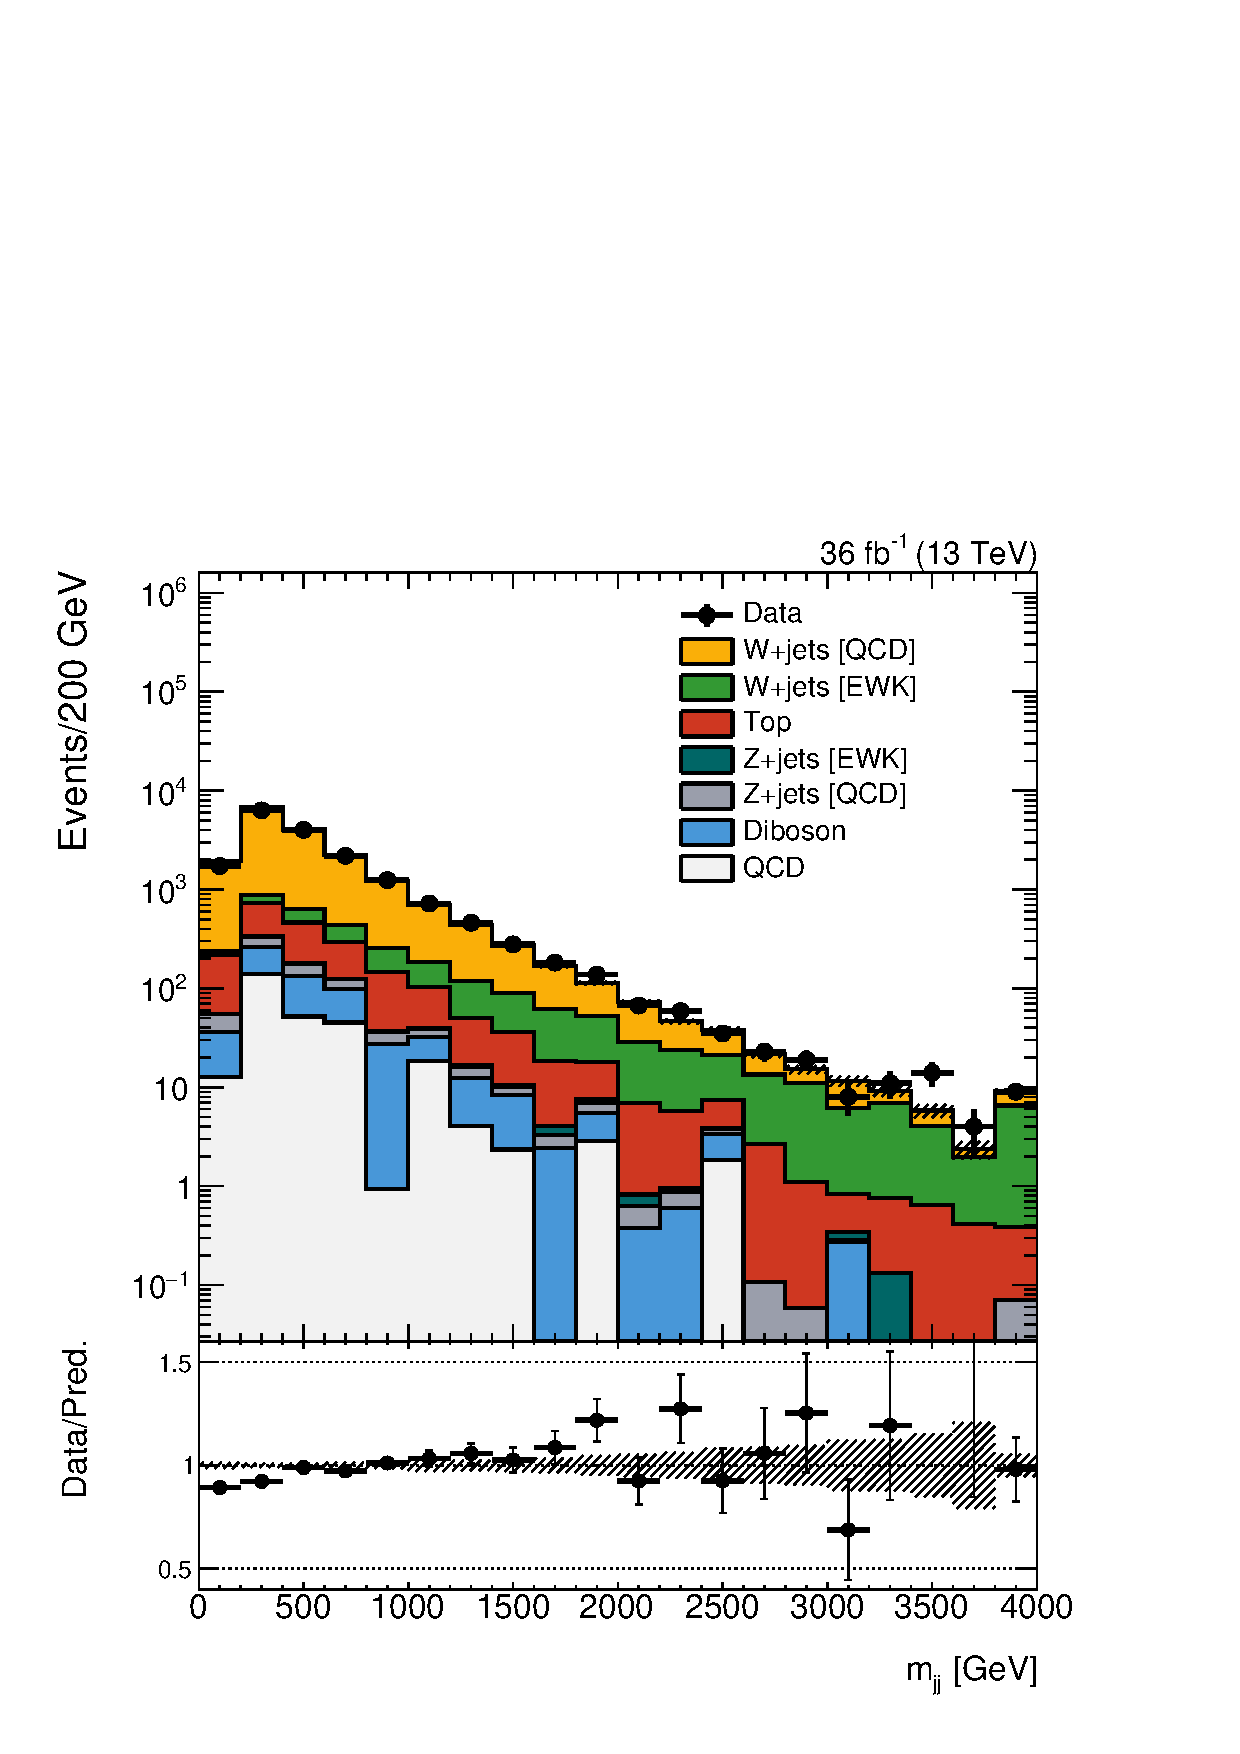
\includegraphics[width=\textwidth]{figures/vbf/prefit/singleelectron_jot12Mass_logy.pdf}
        \end{subfigure}
        \begin{subfigure}[t]{0.24\textwidth}
            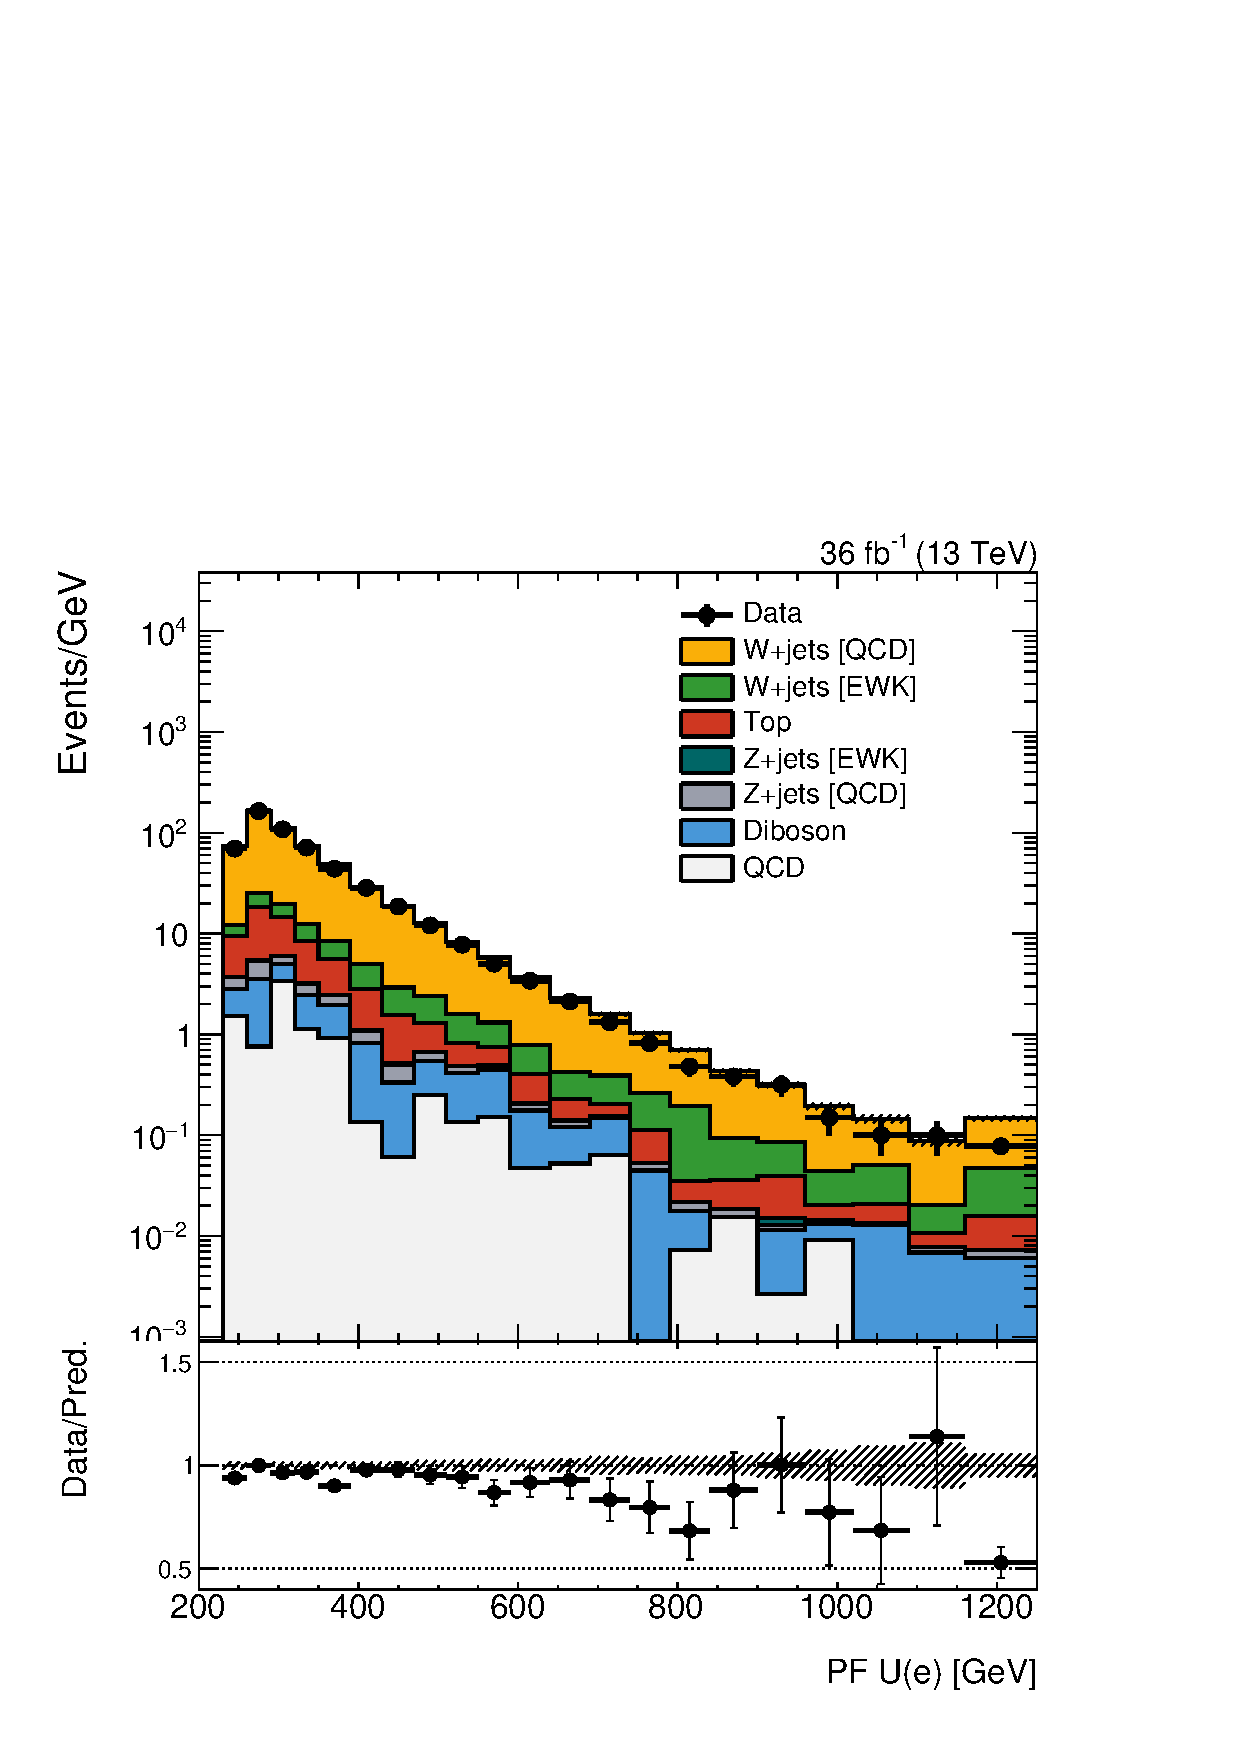
\includegraphics[width=\textwidth]{figures/vbf/prefit/singleelectron_pfUWmag_logy.pdf}
        \end{subfigure} \\ 
        \begin{subfigure}[t]{0.24\textwidth}
            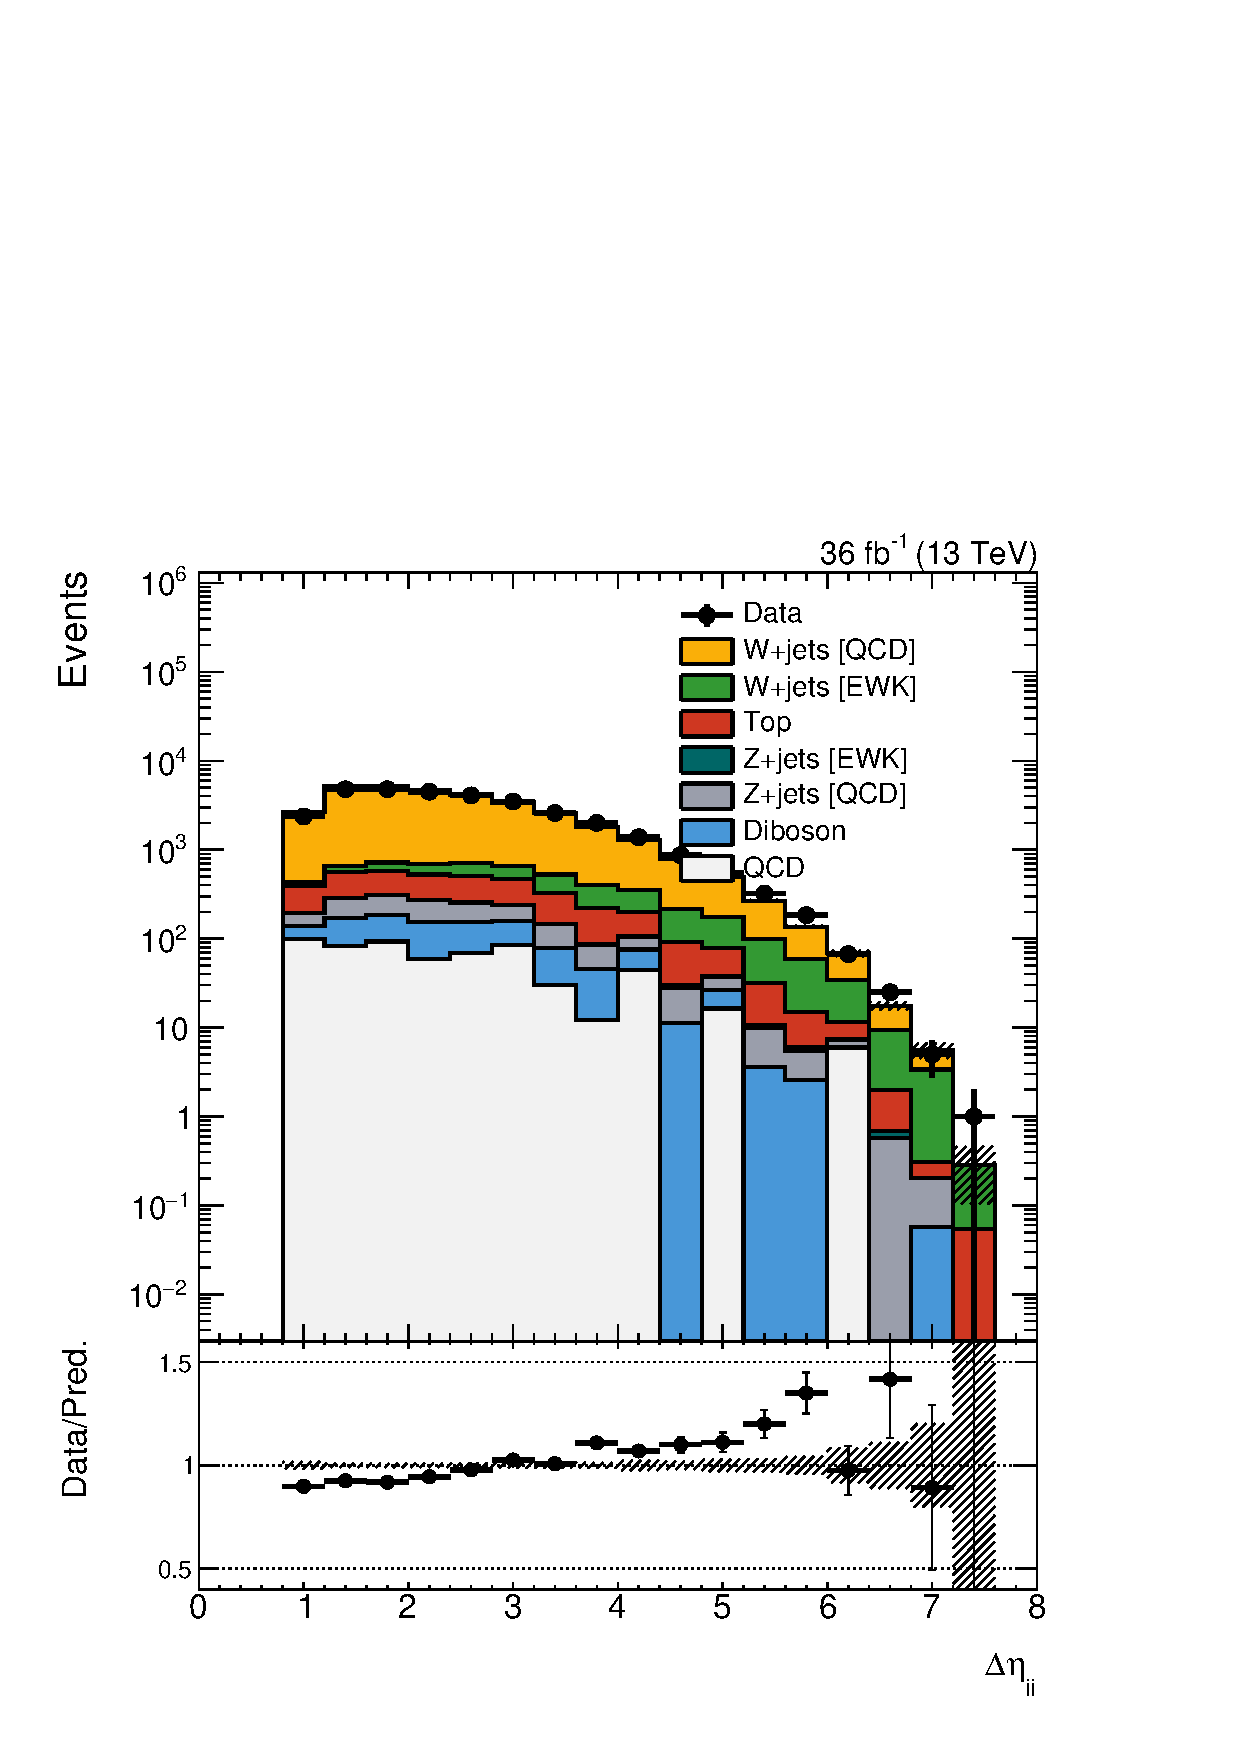
\includegraphics[width=\textwidth]{figures/vbf/prefit/singlemuon_jot12DEta_logy.pdf}
        \end{subfigure}
        \begin{subfigure}[t]{0.24\textwidth}
            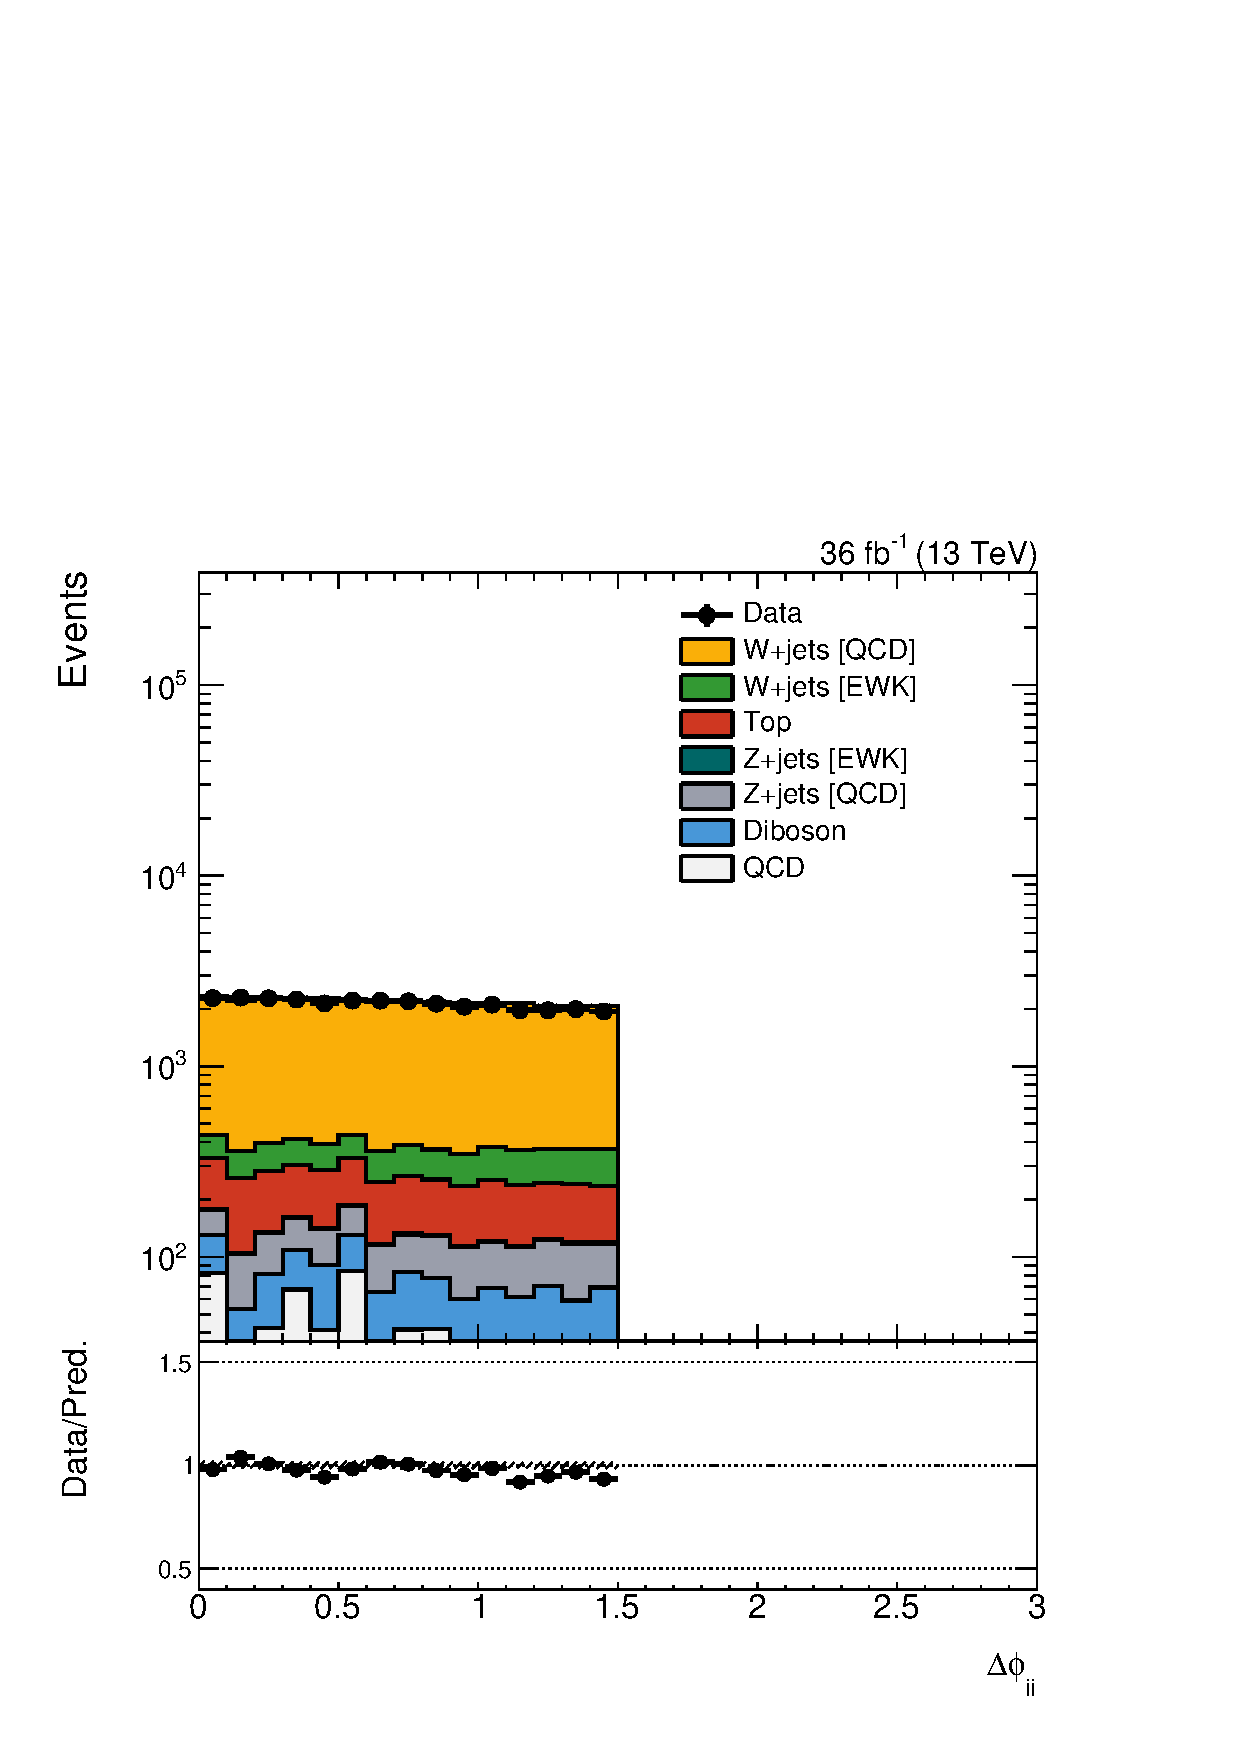
\includegraphics[width=\textwidth]{figures/vbf/prefit/singlemuon_jot12DPhi_logy.pdf}
        \end{subfigure}
        \begin{subfigure}[t]{0.24\textwidth}
            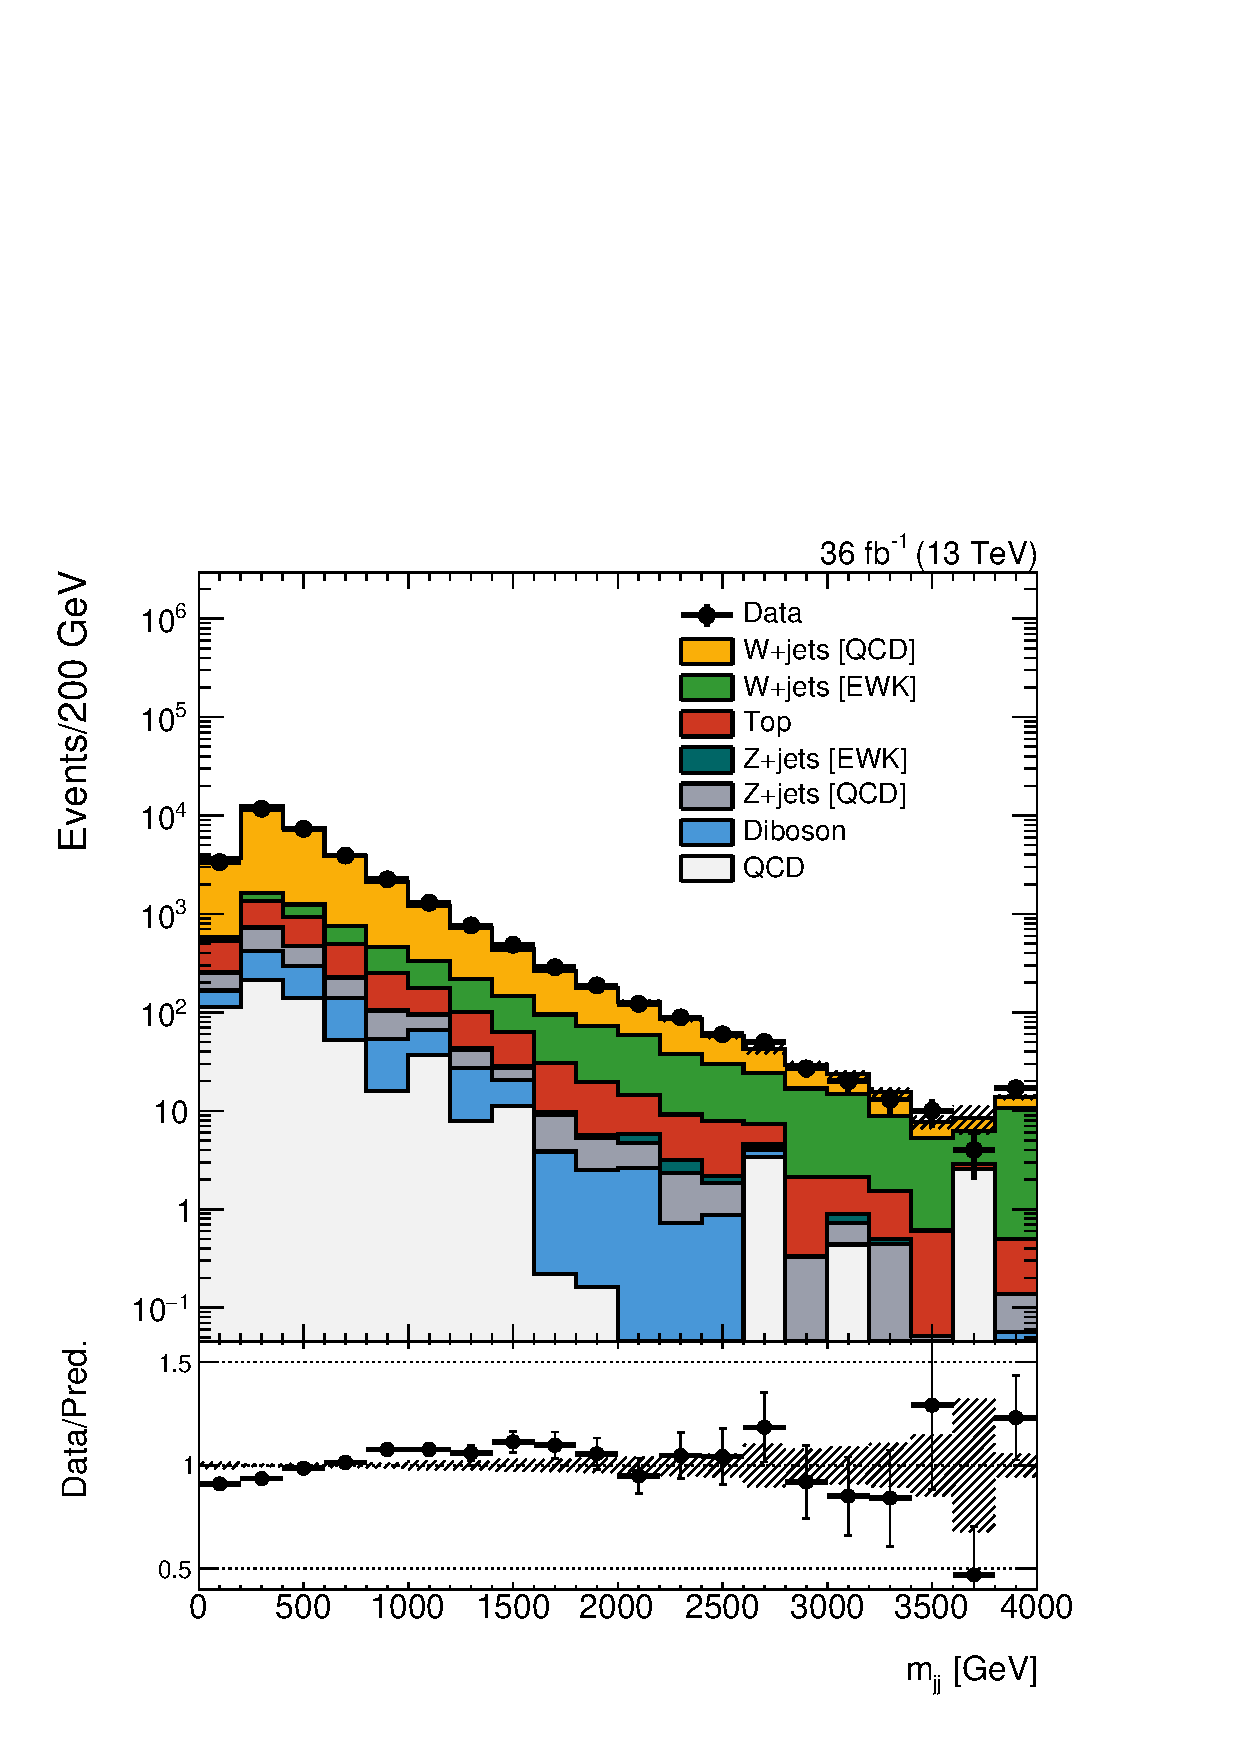
\includegraphics[width=\textwidth]{figures/vbf/prefit/singlemuon_jot12Mass_logy.pdf}
        \end{subfigure}
        \begin{subfigure}[t]{0.24\textwidth}
            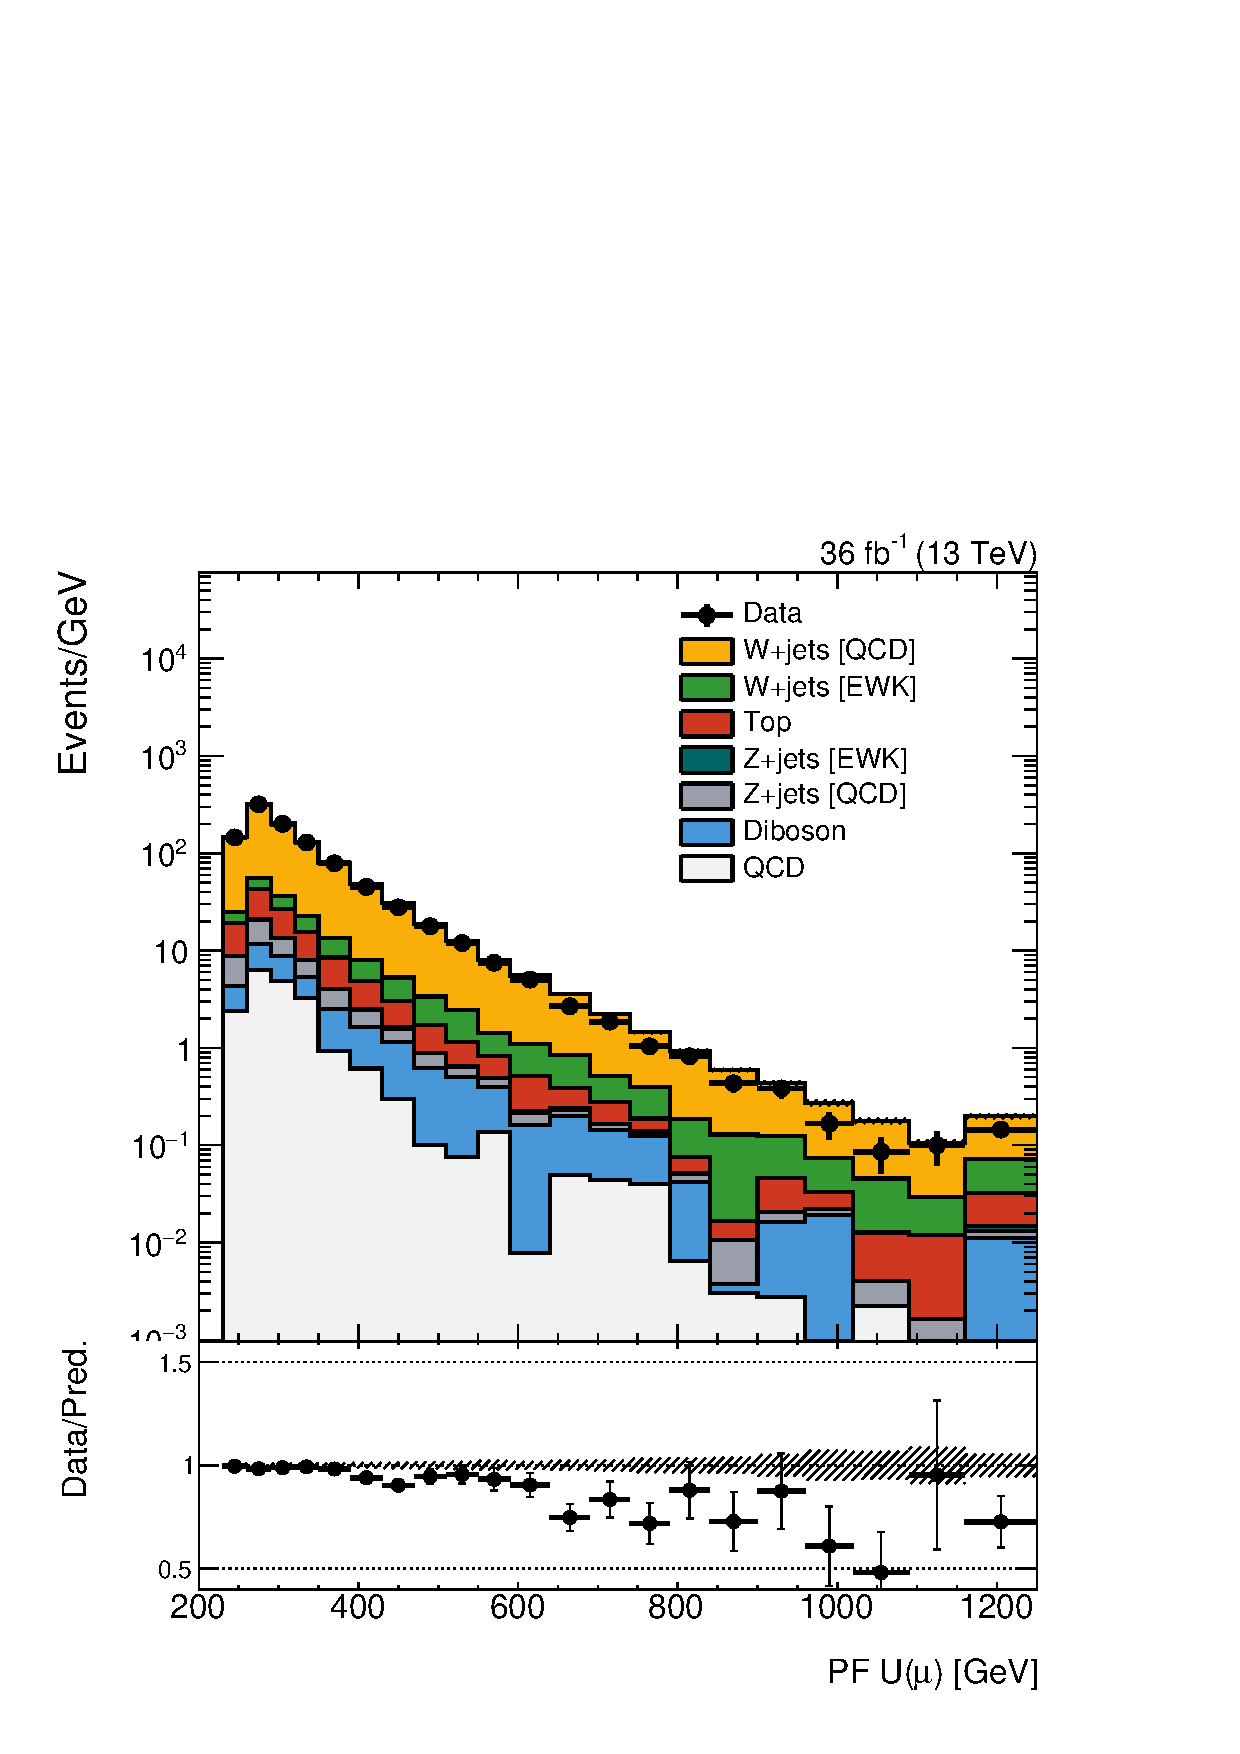
\includegraphics[width=\textwidth]{figures/vbf/prefit/singlemuon_pfUWmag_logy.pdf}
        \end{subfigure}
        \caption{Dijet and recoil distributions in the single-electron (top) and single-muon (bottom) CRs.
                 All predicted distributions are prior to the maximization of the likelihood, and the grey band refers only to the statistical uncertainty of the MC.
                 The pre-fit MC describes the observed data reasonably well.
        }
        \label{fig:vbf:wcr}
    \end{center}
\end{figure}


\begin{figure}[]
    \begin{center}
        \begin{subfigure}[t]{0.32\textwidth}
            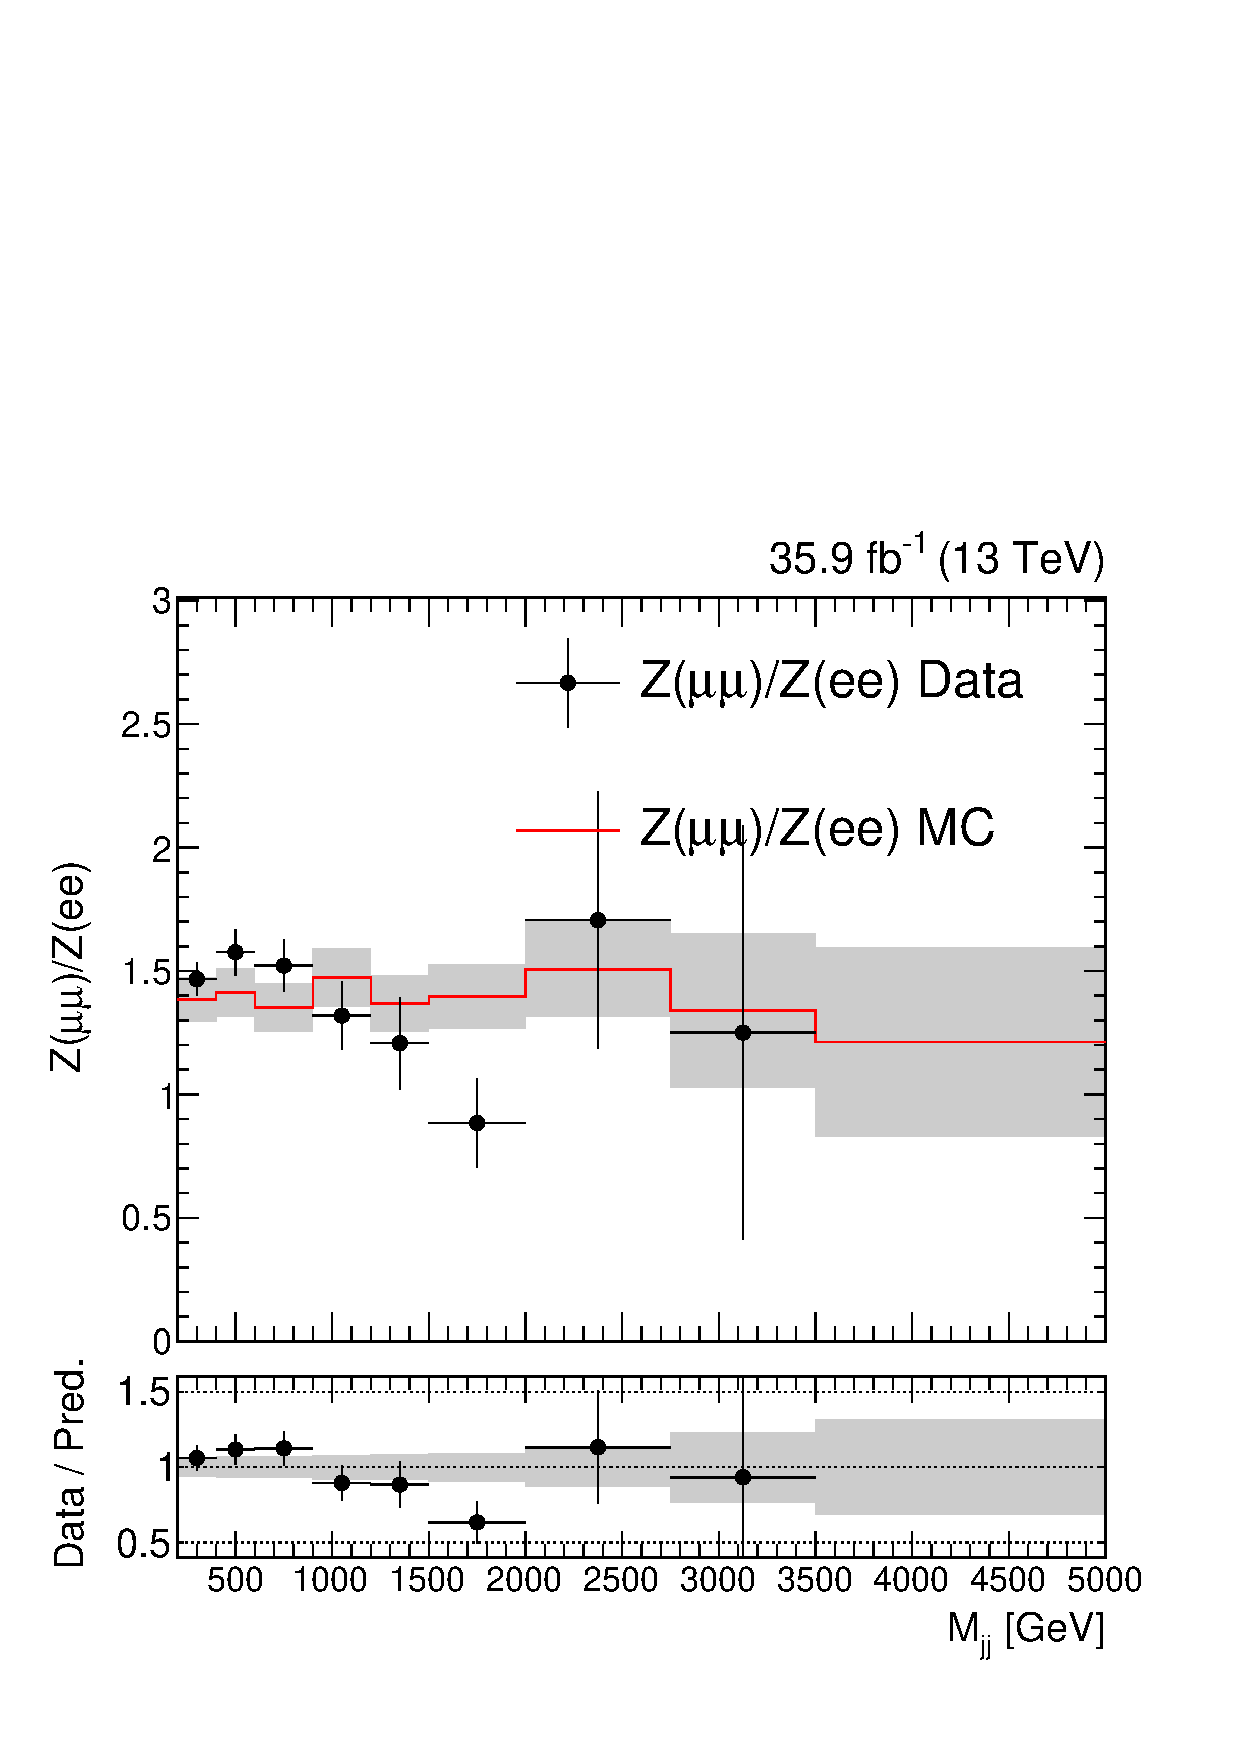
\includegraphics[width=\textwidth]{figures/vbf/fits/dimuon_dielectron_cat_vbf_ratio.pdf}
        \end{subfigure}
        \begin{subfigure}[t]{0.32\textwidth}
            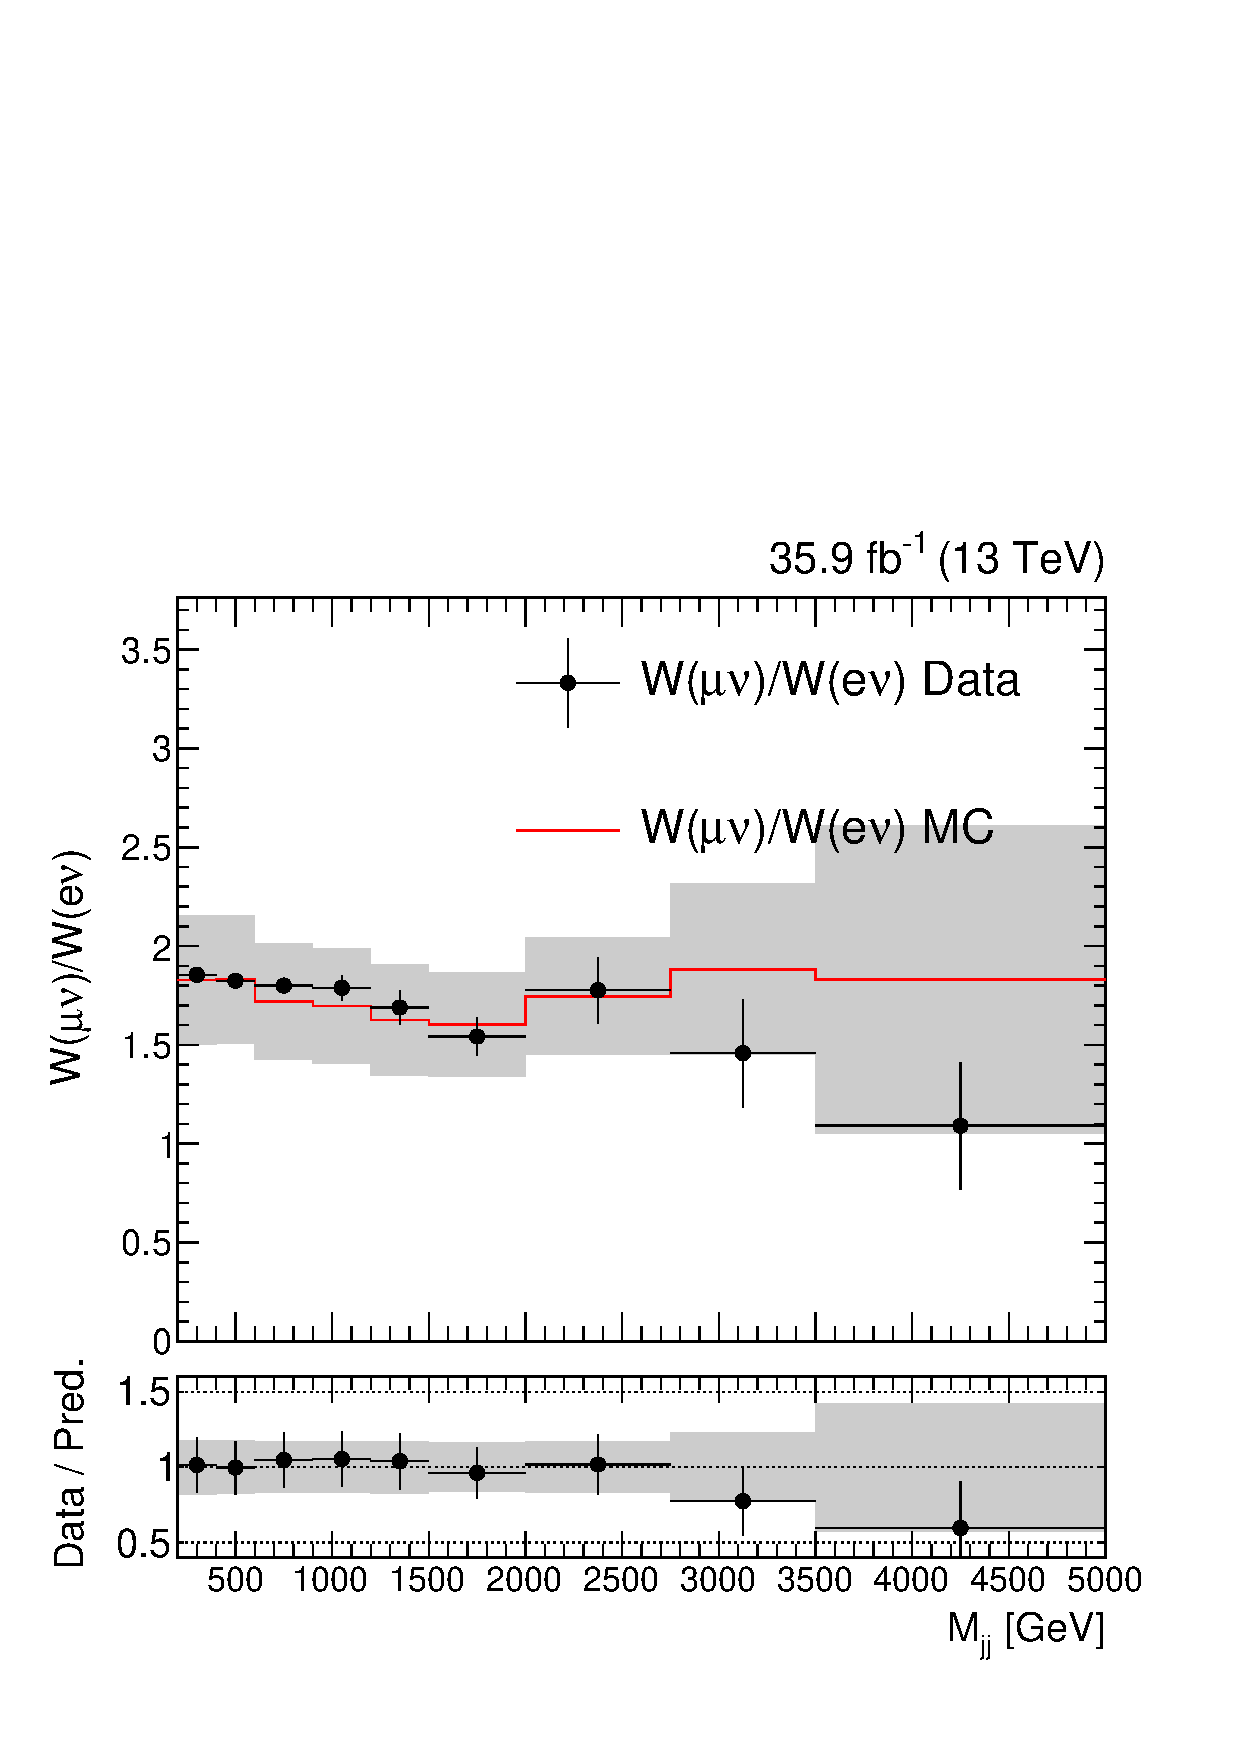
\includegraphics[width=\textwidth]{figures/vbf/fits/singlemuon_singleelectron_cat_vbf_ratio.pdf}
        \end{subfigure}
        \begin{subfigure}[t]{0.32\textwidth}
            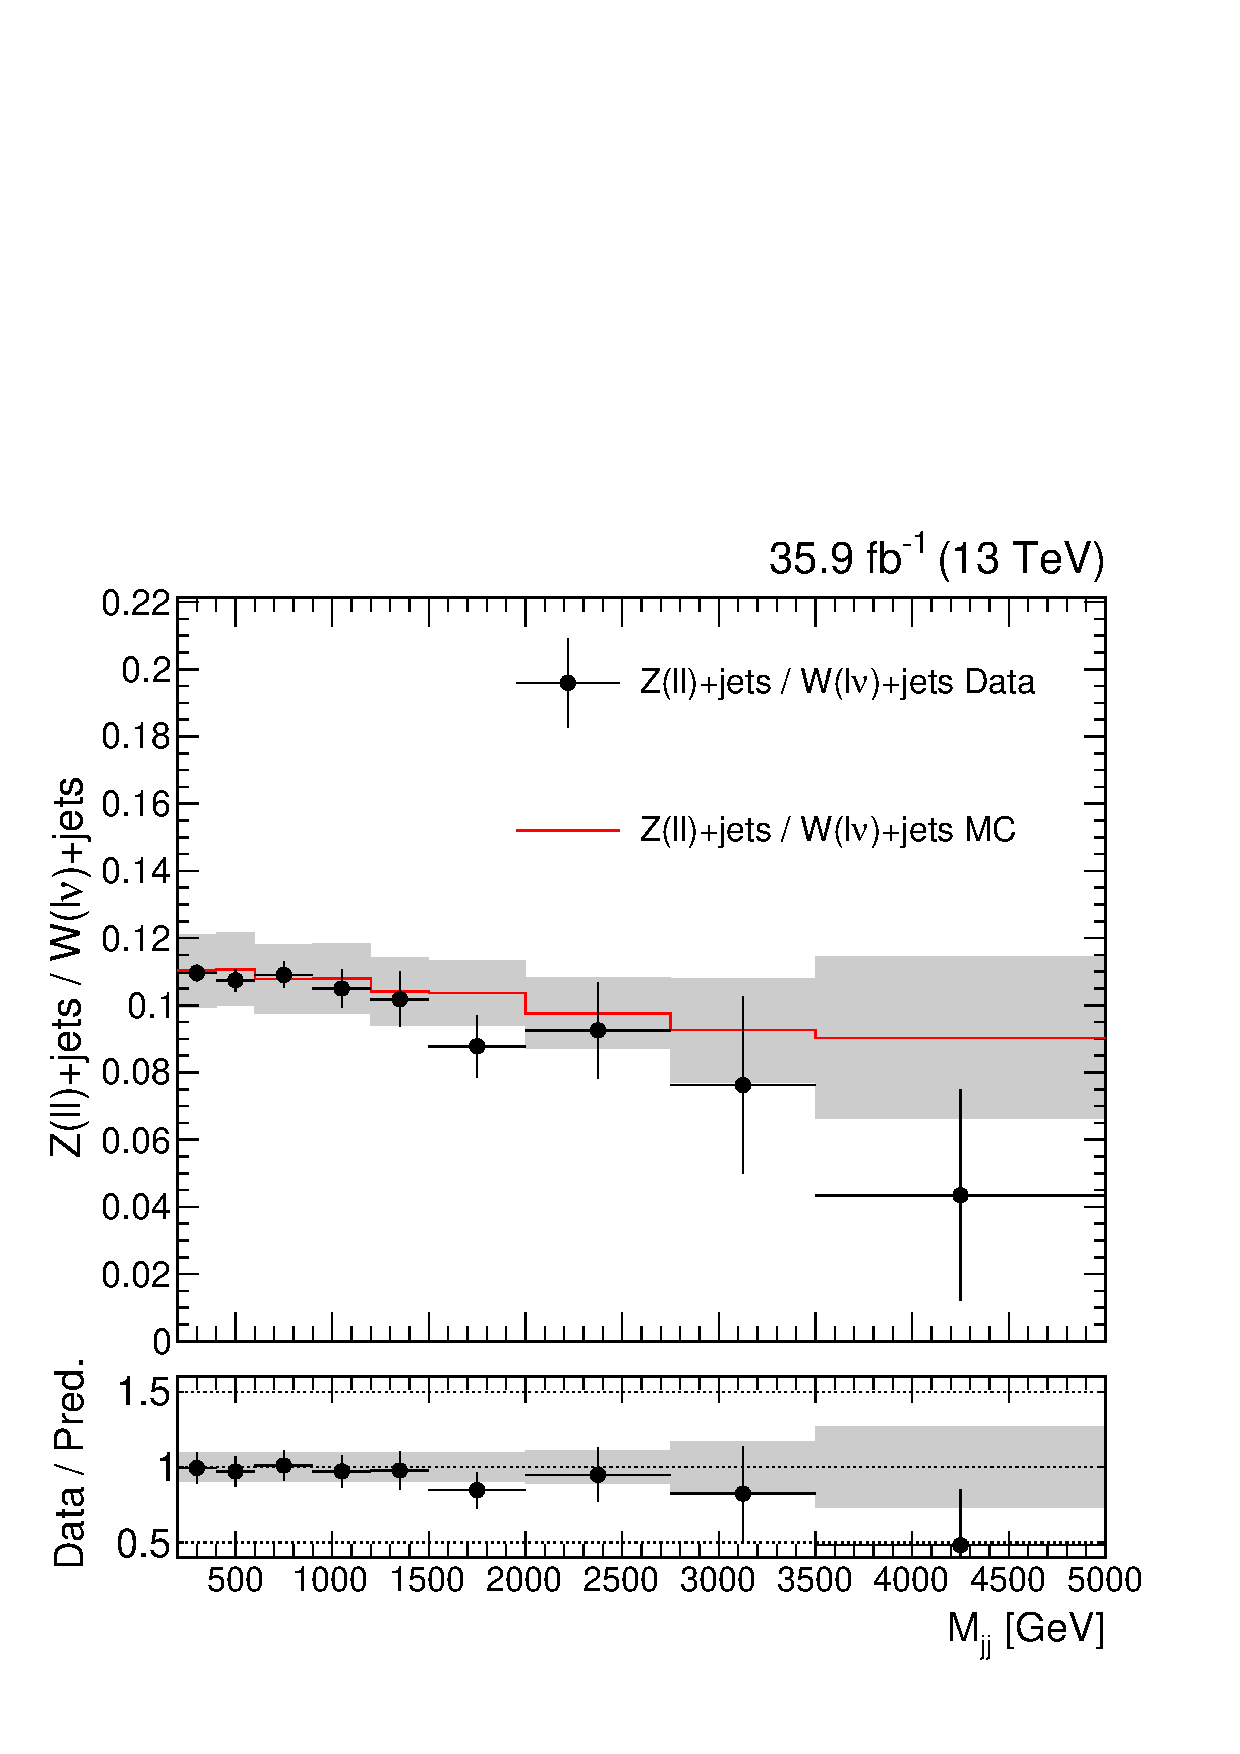
\includegraphics[width=\textwidth]{figures/vbf/fits/combined_combinedW_cat_vbf_ratio.pdf}
        \end{subfigure}
        \caption{Validation of the VBF transfer factors using control region data. 
                 The transfer factor proxies are found to agree quite well with the data within the post-fit uncertainties}
        \label{fig:vbf:valid}
    \end{center}
\end{figure}


\section{Results}

The dijet mass distribution in data is fit in all signal and control regions, the results of which are shown in Figure~\ref{fig:vbf:postfit}.
As no statistically significant excess over the Standard Model is observed, we translate the results into upper limits on the branching ratio of $\hinv$.
As the signal hypothesis, both the VBF and gluon fusion (with 2 extra jets) Higgs production modes are considered; the latter contaminates the SR due to its relatively large cross section.
After the signal region selection criteria, the two modes contribute approximately equal yields. 
Assuming $m_H=125$ GeV, the observed 95\% CL upper limit is 0.33. 
Assuming a background-only hypothesis, the expected distribution of upper limits has median $0.33$, with the 1 standard deviation band covering $[0.18,0.35]$; the observation therefore represents an upwards fluctuation slightly under $1\sigma$. 

\begin{figure}[]
    \begin{center}
        \begin{subfigure}[t]{0.32\textwidth}
            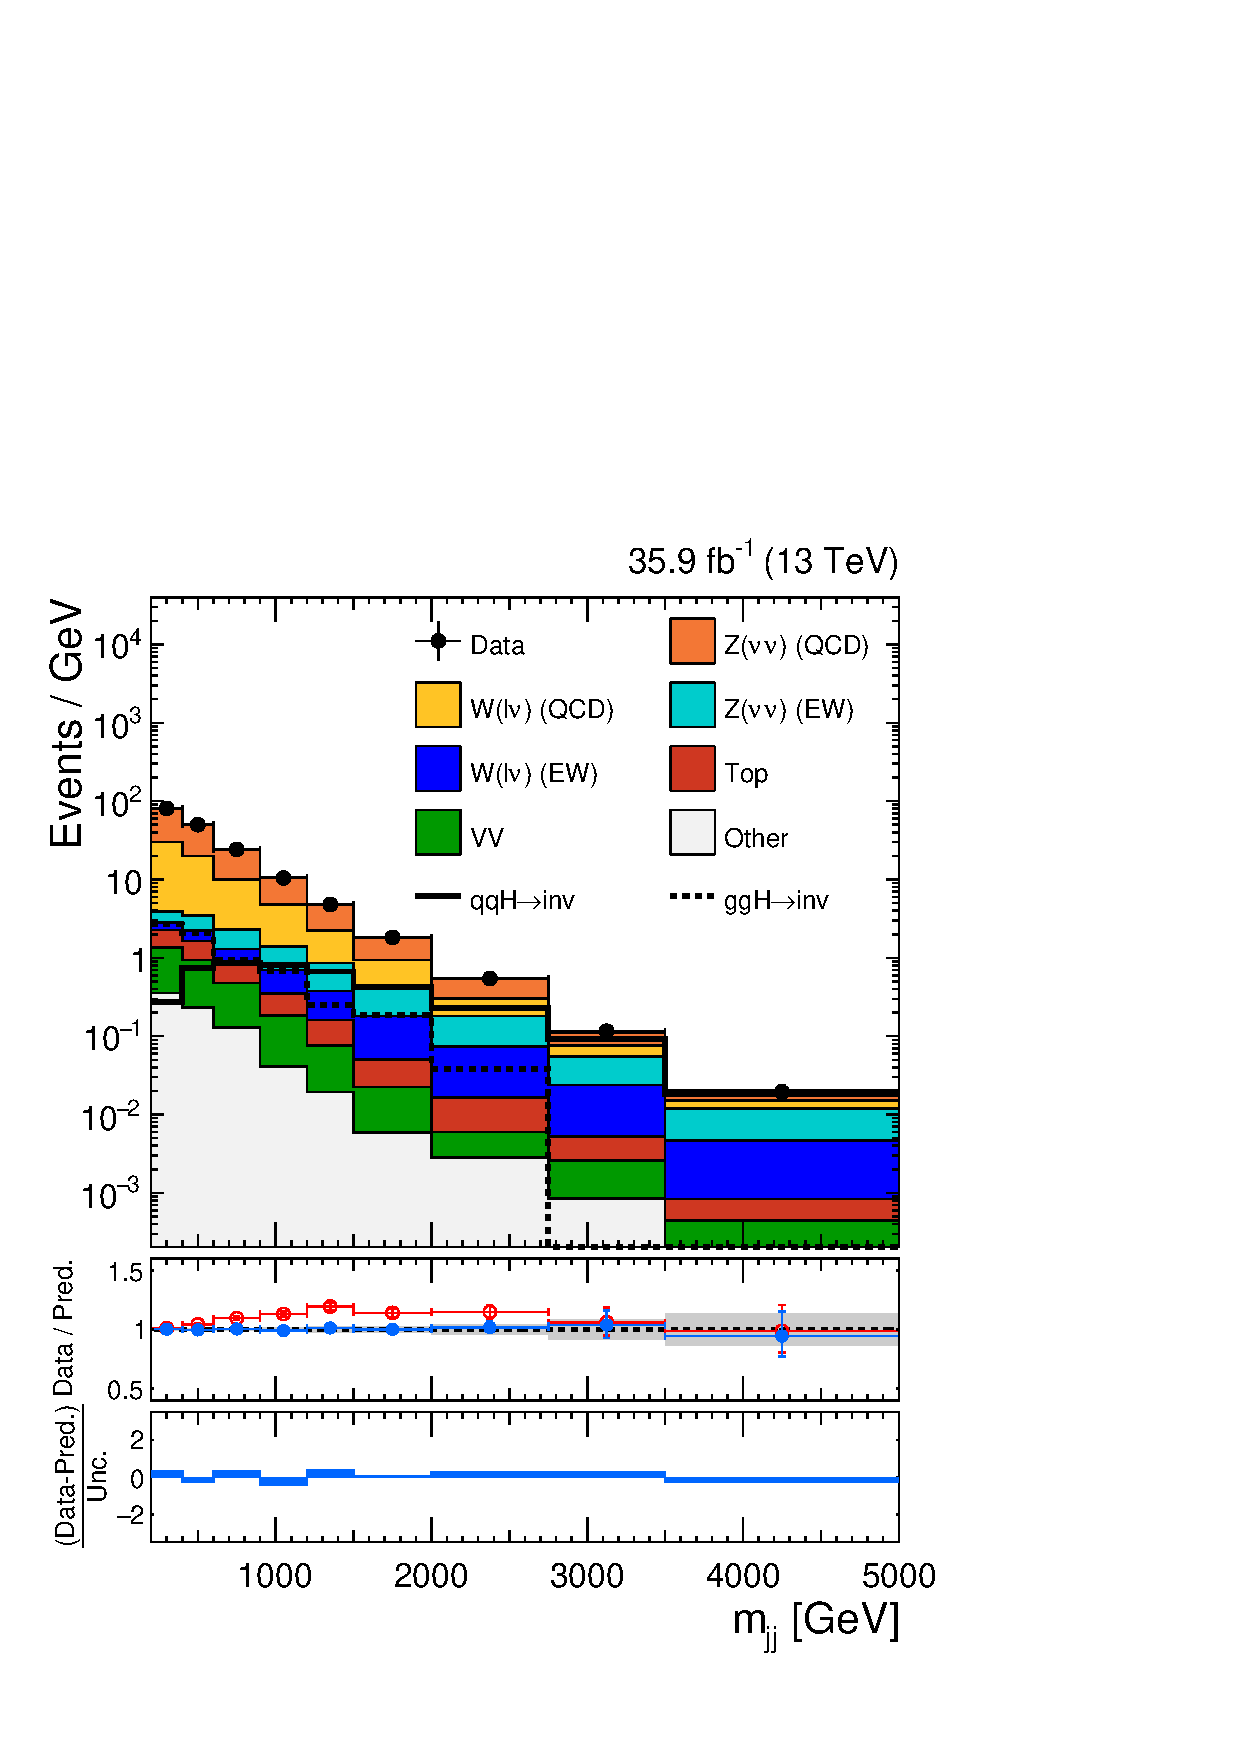
\includegraphics[width=\textwidth]{figures/vbf/fits/vbf_PULLS_prefit_postfit_signal.pdf}
            \caption{SR}
        \end{subfigure}
        \begin{subfigure}[t]{0.32\textwidth}
            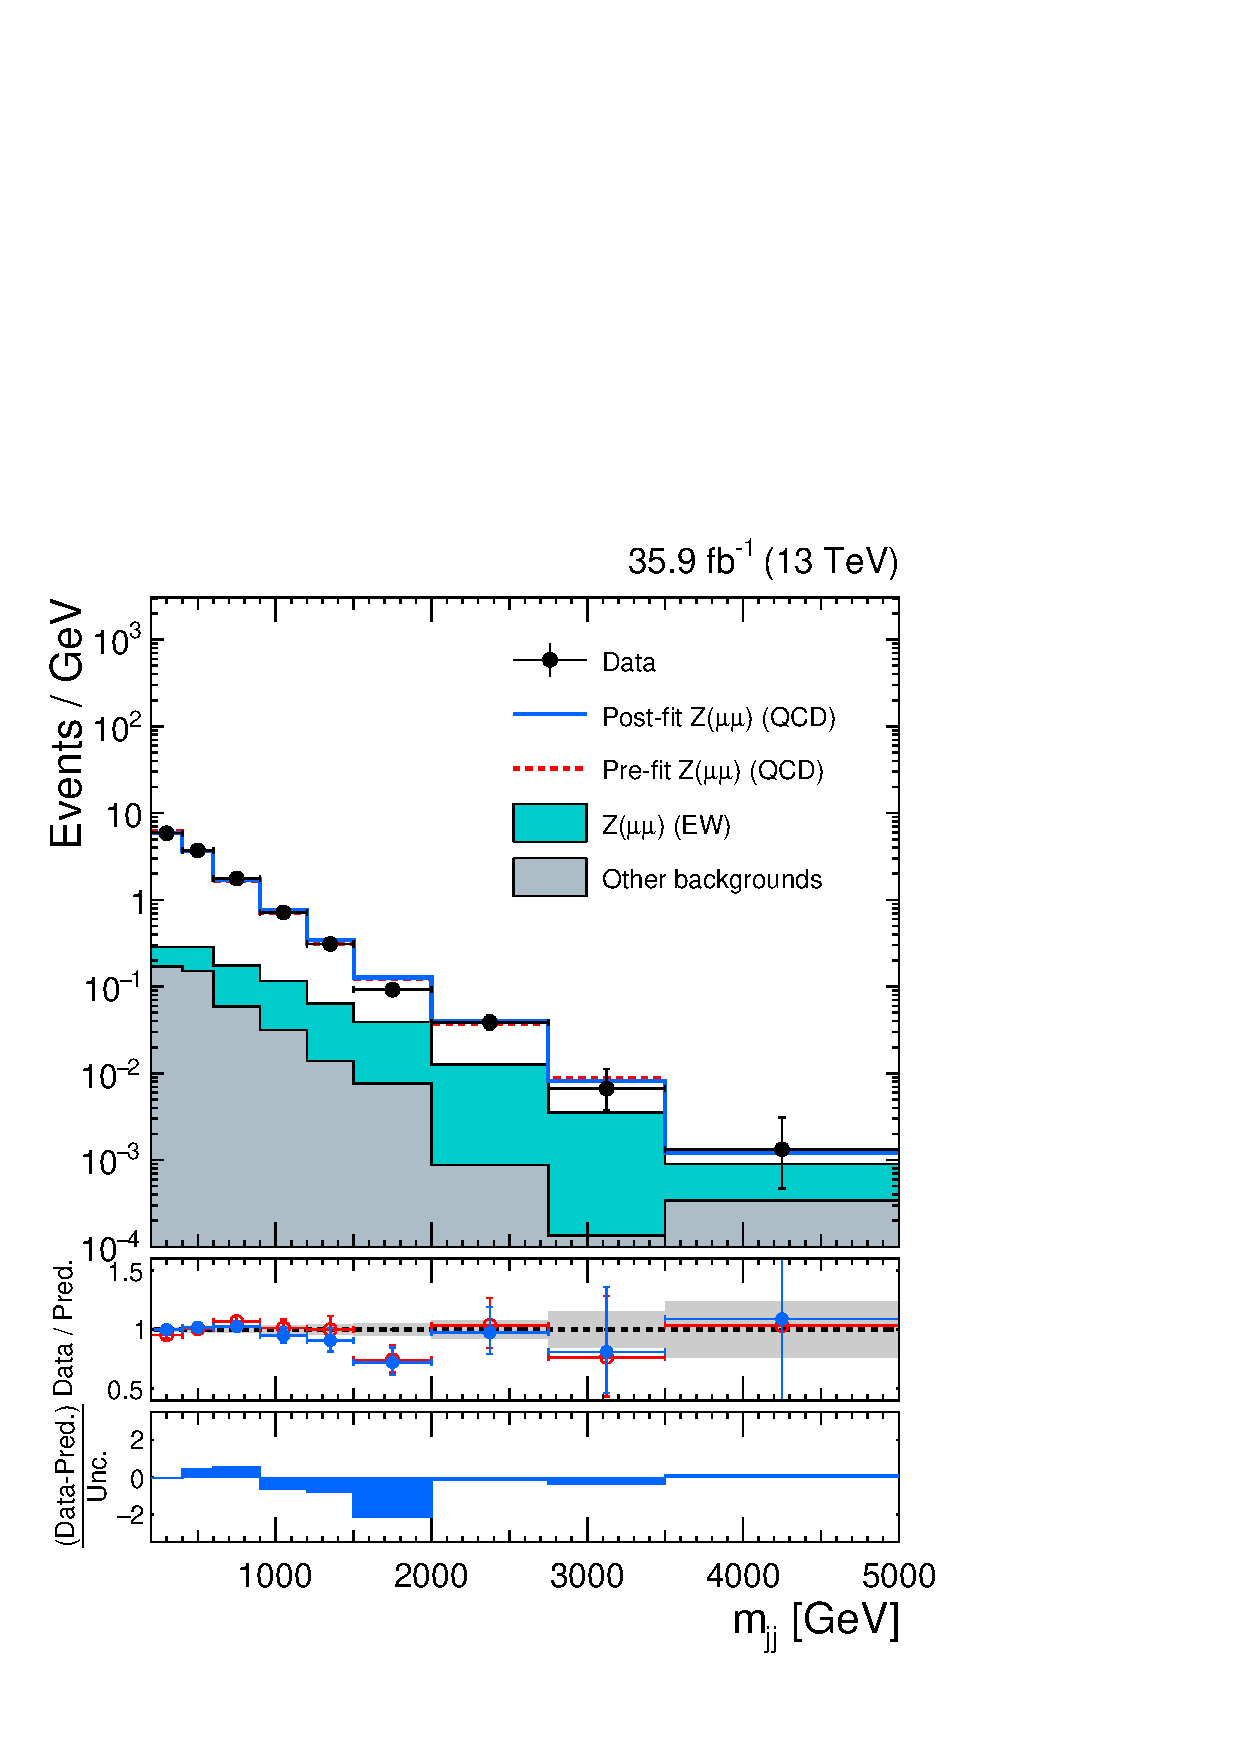
\includegraphics[width=\textwidth]{figures/vbf/fits/vbf_PULLS_prefit_postfit_dimuon.pdf}
            \caption{$\mu\mu$ CR}
        \end{subfigure}
        \begin{subfigure}[t]{0.32\textwidth}
            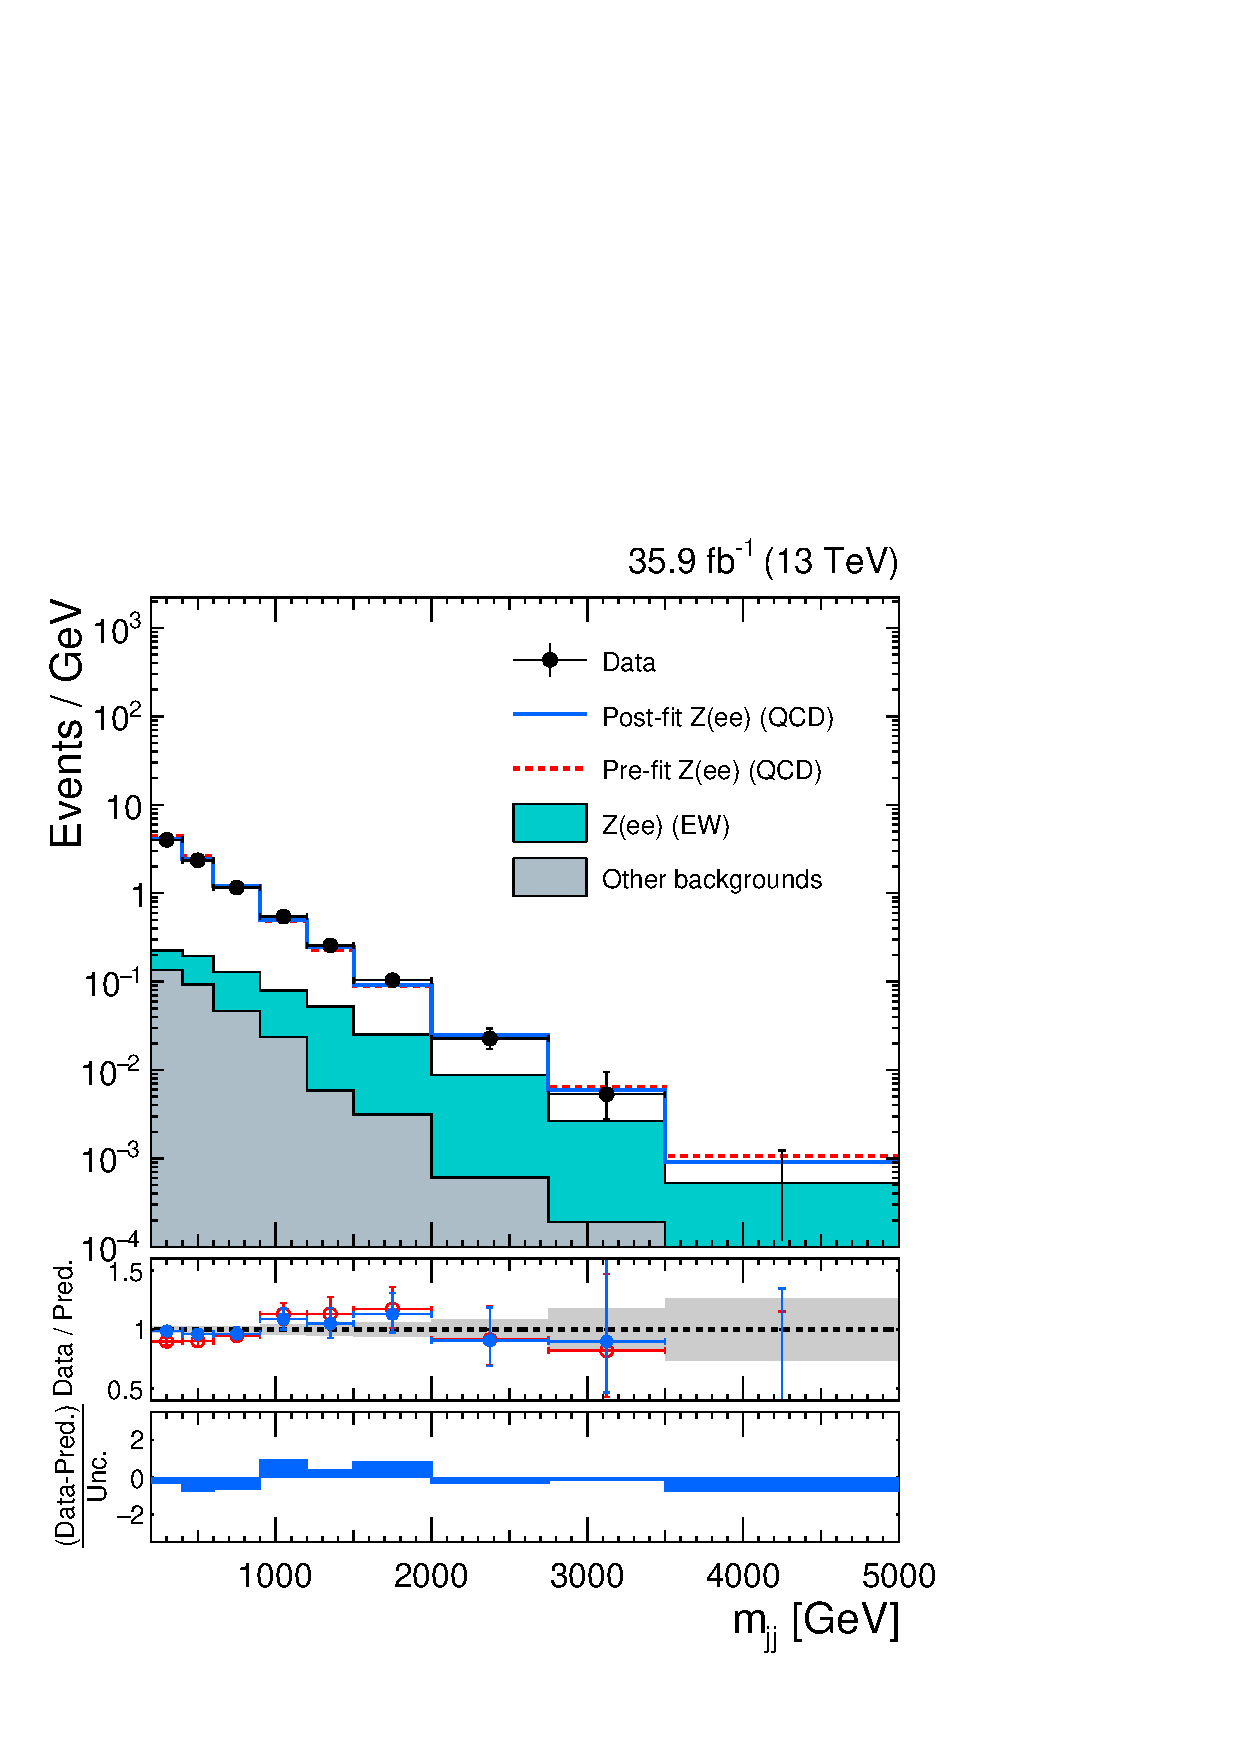
\includegraphics[width=\textwidth]{figures/vbf/fits/vbf_PULLS_prefit_postfit_dielectron.pdf}
            \caption{$ee$ CR}
        \end{subfigure} \\ 
        \begin{subfigure}[t]{0.32\textwidth}
            \includegraphics[width=\textwidth]{figures/vbf/fits/vbf_PULLS_prefit_postfit_singlemuon.pdf}
            \caption{$\mu$ CR}
        \end{subfigure}
        \begin{subfigure}[t]{0.32\textwidth}
            \includegraphics[width=\textwidth]{figures/vbf/fits/vbf_PULLS_prefit_postfit_singleelectron.pdf}
            \caption{$e$ CR}
        \end{subfigure}
        \caption{Post-fit $m_{jj}$ distributions in the various signal and control regions.
                 The uncertainties (gray bands) and bin pulls (blue bands) are defined by varying the nuisances by one standard deviation around the maximum likelihood estimate.}
        \label{fig:vbf:postfit}
    \end{center}
\end{figure}

We further scan $m_H$ and set upper limits on $\sigma(qq\rightarrow qqH)\mathcal{B}(\hinv)$. 
The upper limits are shown in Figure~\ref{fig:vbf:mhscan}, and the observed (expected) limits exclude $m_H<540$ GeV ($635$ GeV) assuming a branching ratio of $100\%$. 

\begin{figure}[]
    \begin{center}
        \includegraphics[width=0.5\textwidth]{figures/vbf/fits/mhscan_ggf.pdf}
        \caption{Upper limits on $\sigma\times \mathcal{B}/\sigma_\mathrm{theory}$ as a function of $m_H$, where $\sigma$ refers to the total production cross section of the Higgs boson with mass $m_H$.
                 If one assumes that $\sigma = \sigma_\mathrm{theory}$, then the upper limits can be interpreted directly as constraints on $\mathcal{B}(\hinv)$.}
        \label{fig:vbf:mhscan}
    \end{center}
\end{figure}

As described in the beginning of this chapter, each Higgs production mode corresponds to a potential invisible Higgs search channel.
While VBF is the most sensitive, the total sensitivity can be improved by statistically combining all channels.
Other results from CMS cover searches for associated production of a Higgs boson, either with a leptonically-decaying $Z$ boson \cite{zhinv} or a hadronically-decaying weak boson \cite{monojet}; and for gluon fusion production, with at least one jet originating from the initial state or heavy quark loop \cite{monojet}. 
The details of these searches are left to the referenced literature, but a summary of their results is provided in Figure~\ref{fig:vbf:comb}.
When statistically combining the results, most experimental nuisances are treated as correlated between the searches, with the exception of the VBF jet energy scale dependence.
This is because the VBF category selects forward jets, whereas other searches generally probe central jets.
Theoretical nuisances, such as those affecting $W/Z$ or $ZZ/WZ$ ratios, are left uncorrelated between all searches.
The combined result constrains $\mathcal{B}(\hinv)$ to be less than $0.26$ at 95\% CL, which approximately corresponds to a 1 standard deviation fluctuation upward relative to the median expected limit of $0.20$.

\begin{figure}[]
    \begin{center}
        \includegraphics[width=0.6\textwidth]{figures/vbf/fits/comb.pdf}
        \caption{Upper limits on $\mathcal{B}(\hinv)$ after statistically combining all of the CMS searches for $\hinv$~conducted on $36$ fb$^{-1}$ of data collected in 2016.
                 For comparison, the upper limits of each of the individual categories are also shown.}
        \label{fig:vbf:comb}
    \end{center}
\end{figure}

Higgs-mediated DM can also be probed by direct detection (DD) experiments.
We interpret the combined 90\% CL upper limit on $\mathcal{B}(\hinv)$ as an upper limit on the spin-independent cross section of DM-nucleon scattering. 
First, we convert the branching ratio into a partial width:
\begin{equation}
    \Gamma_{\hinv} = \frac{\mathcal{B}(\hinv) \cdot \Gamma_\mathrm{SM}}{1 - \mathcal{B}(\hinv)}, \text{ where }\Gamma_\mathrm{SM} = 4~\mathrm{GeV}
\end{equation}
Then, using the results described in Reference~\cite{higgsdm3}, $\Gamma_{\hinv}$ is translated into $\sigma^{\mathrm{SI}}_{\chi N}(m_\chi)$, where the only free parameter is the DM mass.
Figure~\ref{fig:vbf:dd} compares the CMS exclusions with those from DD experiments~\needcite.
Also shown for comparison is the \emph{neutrino floor}, which is the cross section of coherent scattering of solar neutrinos, and a limiting factor for DD experiments.
At low $m_\chi$, CMS is able to significantly extend the DD constraints, reaching well below the neutrino floor. 

\begin{figure}[]
    \begin{center}
        \includegraphics[width=0.5\textwidth]{figures/vbf/fits/dd.pdf}
        \caption{Upper limits on $\sigma^\mathrm{SI}_{\chi N}$ as a function of $m_\chi$. 
                 Shown are the combined results from the CMS invisible Higgs searches, as well as various direct detection experiments.}
        \label{fig:vbf:dd}
    \end{center}
\end{figure}

